% !Mode:: "Tex:UTF-8"

\section{Primeras nociones sobre Probabilidad.}
\label{cap03:sec:PrimerasNocionesProbabilidad}
\label{PrimerasNocionesProbabilidad}


El estudio de la Probabilidad nació, como disciplina científica, en el siglo XVII y en relación con los juegos de azar y las apuestas. Y es en ese contexto, de lanzar monedas, y de juegos con dados, cartas y ruletas, donde todavía se siguen encontrando la mayoría de los ejemplos con los que se presenta la teoría a quienes se inician en su estudio. Nosotros vamos a hacer lo mismo.
    \begin{enumerate}
        \item Lanzamiento de dados: cuando se lanzan unos dados (sin trucar), el resultado de cada lanzamiento individual es imposible de predecir. Se observa, tras realizar un número muy grande de lanzamientos, que cada uno de los seis posibles resultados aparece aproximadamente una sexta parte de las veces.
        \item Lanzamiento de monedas: del mismo modo, cuando se lanza una moneda (sin trucar), se observa, al cabo de muchos lanzamientos, que cada uno de los dos posibles resultados aparece aproximadamente la mitad de las veces.
        \item Las loterías, con la extracción de bolas numeradas de una urna o un bombo giratorio; o la ruleta, en la que la bola que se lanza puede acabar en cualquiera de las 36 (o 37) casillas.  Estos juegos y otros similares, ofrecían ejemplos adicionales con elementos comunes a los anteriores.
    \end{enumerate}
Las apuestas, basadas en esos juegos de azar, y los casinos son, desde antiguo, un entretenimiento muy apreciado. Para hacer más interesante el juego, la humanidad fue construyendo otros juegos combinados más complicados. Por ejemplo, apostamos cada uno un euro y lanzamos dos dados: si la suma de los resultados es par, yo me llevo los dos euros. Si es impar, los ganas tú. La pregunta es evidente ¿Es este un juego {\em justo} para ambos jugadores? En concreto, lo que queremos saber es: si jugamos muchas, muchas veces ¿cuántos euros perderé o ganaré yo en promedio por cada euro invertido? ¿Y cuántos ganarás o perderás tú? Está claro que para que un jugador esté dispuesto a participar, y a arriesgar su fortuna, y desde luego para que alguien considere rentable el casino como negocio, o la lotería como forma de recaudar dinero, es preciso ofrecerle {\sf información precisa sobre cuáles son las ganancias esperadas del juego}. Uno de nuestros objetivos es aprender a responder a esa pregunta: ¿cómo se calculan las ganancias esperadas? No es una pregunta tan específica de los juegos de azar como pueda parecer a primera vista. En general, cuando nos enfrentamos a un fenómeno aleatorio, ¿cuáles son los resultados esperables? ¿Cómo podemos hacer medible nuestra incertidumbre sobre esos resultados?

\subsubsection*{}
Otra cosa que la humanidad constató rápidamente al tratar con los juegos de azar es que, como hemos
dicho en la introducción a esta parte del curso, nuestra intuición, en este terreno, es
especialmente débil. Las personas en general, tendemos a subestimar o sobrevalorar mucho las
probabilidades de muchos fenómenos. Y así consideramos como milagros algunos fenómenos
perfectamente normales y predecibles, o viceversa. Uno de nuestros ejemplos favoritos de lo
engañosa que puede ser nuestra intuición cuando se trata de probabilidades, es el que se conoce
como {\sf problema de Monty Hall}\index{problema de Monty Hall}\index{Monty Hall, problema de},
sobre el que puedes leer en el enlace [\,\ref{enlace0004}\,]\label{enlace0004a}.
En el Episodio 13 de la primera temporada de la serie de televisión Numb3rs (más información en el
enlace [\,\ref{enlace0005}\label{enlace0005a}\,]),  se ilustra
este problema de una forma muy entretenida. Recomendamos encarecidamente al lector que, si tiene
ocasión, no deje de ver ese fragmento en particular.
%
%en esta clase vamos a ver un vídeo de un fragmento  de la serie de televisión \link{http://en.wikipedia.org/wiki/Numb3rs}{Numb3rs} en el que se describe  En Moodle tenéis un enlace al vídeo por si queréis volver a verlo.\\[3mm]

Otro ejemplo pertinente, que además tiene interés histórico, es el que se describe en detalle (y
con humor) en el Capítulo 3 del libro {\em La Estadística en Comic} de Gonick y Smith (ver
referencia \cite{EstadisticaComic} de la Bibliografía), como {\sf Problema del Caballero de
Méré}\index{Méré, problema del caballero de}\index{Caballero de Méré, problema de}\index{problema
del caballero de Méré} (más información en el enlace [\,\ref{enlace0006}\,].\label{enlace0006a}): ¿qué
es más probable?
    \begin{itemize}
    \item[(a)] obtener al menos un seis en cuatro tiradas de un dado, o
    \item[(b)] obtener al menos un seis doble en 24 tiradas de dos dados?
    \end{itemize}
    Los jugadores que, en aquella época, se planteaban esta pregunta respondían inicialmente así:
    \begin{itemize}
    \item[(a)] La probabilidad de obtener un seis en cada tirada es $\dfrac{1}{6}$. Por lo tanto, en cuatro tiradas es
    \[\dfrac{1}{6}+\dfrac{1}{6}+\dfrac{1}{6}+\dfrac{1}{6} = \dfrac{2}{3}.\]

    \item[(b)] La probabilidad de obtener un doble seis en cada tirada de dos dados es $\dfrac{1}{36}$, porque hay 36 resultados distintos, y todos aparecen con la misma frecuencia. Por lo tanto, en veinticuatro tiradas será \[\dfrac{1}{36}+\cdots+\dfrac{1}{36}=\dfrac{24}{36}=\dfrac{2}{3}.\]
    \end{itemize}
Así que en principio ambas apuestas son iguales, y las cuentas parecen indicar que recuperaríamos dos de cada tres euros invertidos (el 66\%). Sin embargo, no es así, como algunos de esos jugadores debieron experimentar dolorosamente en sus patrimonios.

Uno de nuestros objetivos en este curso es animar al lector a que ponga a prueba sus ideas, y considere a la Estadística, en buena medida, como una ciencia {\em experimental}. Eso es posible en muchos casos recurriendo al ordenador. Por esa razón, en el Tutorial03 vamos a ver cómo podemos usar el ordenador para simular un gran número de partidas de las dos apuestas del Caballero de Méré. Repetimos que la ganancia esperada es de un 66\% de lo invertido. Y lo que se observa es que la proporción de apuestas perdidas frente a apuestas ganadas no es, ni la que esperábamos, ni siquiera es igual en ambos casos. De hecho, dentro de poco vamos a aprender a calcular los valores correctos, y veremos que para la apuesta (a) ese valor es aproximadamente $0.52$, mientras que para la apuesta (b) es aproximadamente $0.49$.
%
%
%Para ilustrar lo que decimos, vamos a utilizar aquí dos hojas de cálculo, llamadas \fichero{../datos/Cap03-DeMere1.ods}{{Cap03-DeMere1.ods}} (para la apuesta (a)) y \fichero{../datos/Cap03-DeMere2.ods}{{Cap03-DeMere2.ods}} (para la apuesta (b))\label{cap03:lugar:hojasCalculoDeMere}, en las que hemos {\em simulado} esas dos apuestas, y hemos jugado 1000 veces cada una de ellas.


\section{Regla de Laplace.}
\label{cap03:sec:ReglaLaplace}

Lo que tienen en común todas las situaciones que hemos descrito, ligadas a juegos de azar, es que:
        \begin{enumerate}
            \item Hay una lista de resultados individuales posibles: los seis números que aparecen en las caras de un dado, las dos caras de la moneda, las 36 casillas de la ruleta francesa, etc. Estos resultados se llaman {\sf resultados elementales}.
            \item Si repetimos el experimento muchas veces (muchos millones de veces si es
                necesario), y observamos los resultados, comprobamos que la {\em frecuencia
                relativa} de aparición de cada uno de los resultados elementales es la misma para
                todos ellos: $1/6$ para cada número en el dado, $1/2$ para cada cara de la
                moneda, $1/36$ para cada casilla de la ruleta. En ese caso decimos que los
                sucesos elementales son \index{sucesos equiprobables}{\sf
                equiprobables}\footnote{Aunque, en la realidad, las cosas no son tan sencillas.
                Quizá os resulte interesante buscar en Internet información sobre la relación
                entre la ruleta y la familia Pelayo.}.
        \end{enumerate}

En este contexto, Pierre Simon Laplace\index{Laplace} (más información sobre él en el enlace
[\,\ref{enlace0003}\label{enlace0003a}\,]),
uno de los mayores genios matemáticos de la Ilustración francesa, desarrolló la que seguramente es
la primera contribución verdaderamente científica al análisis de la Probabilidad, y que en su honor
se conoce como \index{regla de Laplace}{\sf Regla de Laplace.} Vamos a fijar el lenguaje necesario
para formular esa regla.
    \begin{itemize}
        \item[(a)]  Estamos interesados en un {\sf fenómeno o experimento aleatorio}. Es decir, que sucede al azar; como lanzar una moneda, un dado o un par de dados, etc. Y suponemos que ese experimento tiene $n$ {\sf resultados elementales} diferentes:
            \[\{a_1,a_2,\ldots,a_n,\}\]
            y que esos resultados elementales son {\sf equiprobables}, en el sentido de la igualdad de las frecuencias relativas que hemos descrito, cuando el experimento se repite muchas veces.

        \item[(b)]  Además, definimos un {\sf suceso aleatorio}, llamémoslo $A$, que es un resultado, posiblemente más complejo, que se puede definir en términos de los resultados elementales del experimento en (a). Por ejemplo, si lanzamos un dado, $A$ puede ser: obtener un número par. O, si lanzamos dos dados, $A$ puede ser: que la suma de los números sea divisible por $5$. En cualquier caso, en algunos de los resultados elementales ocurre $A$ y en otros no. Eso permite pensar en $A$ como un {\sf subconjunto del conjunto de resultados elementales}. Y aquellos resultados elementales en los que se observa $A$ se dice que son {\sf resultados favorables} al suceso $A$. Por ejemplo, si lanzamos un dado, los resultados favorables al suceso $A=$ {\em(obtener un número par)} son $\{2,4,6\}$. Y podemos decir, sin riesgo de confusión, que $A=\{2,4,6\}$.
    \end{itemize}

Con estas premisas, la formulación de la Regla de Laplace es esta:
        \begin{center}
        \fcolorbox{black}{Gris025}{
        \begin{minipage}{10cm}
            \begin{center}
						{\bf Regla de Laplace.}
						\end{center}
            La probabilidad del suceso A es el cociente:
            \begin{equation}
            \label{cap03:ecu:ReglaLaplace}
            P(A)=\dfrac{\mbox{número de sucesos elementales favorables a $A$}}{\mbox{número total de sucesos elementales}}
            \end{equation}
        \end{minipage}}
        \end{center}
%
%
%
%
%
%
%    \begin{center}
%        \fbox{\colorbox{Gris025}{
%        \begin{minipage}{13cm}
%    \begin{center}
%        {\bf Regla de Laplace: } \\[3mm]
%                \end{center}
%        La probabilidad del suceso A es el cociente:
%        \[p(A)=\dfrac{\mbox{número de sucesos elementales favorables a $A$}}{\mbox{número total de sucesos elementales}}
%        \]
%        \end{minipage}}
%        }
%    \end{center}
La Regla de Laplace supuso un impulso definitivo para la teoría de la Probabilidad, porque hizo posible comenzar a calcular probabilidades y obligó a los matemáticos, a la luz de esos cálculos, a pensar en las propiedades de la probabilidad. Además, esa regla se basa en el recuento de los casos favorables al suceso $A$ de entre todos los posibles. Y eso obliga a desarrollar técnicas de recuento a veces extremadamente sofisticadas (contar es algo muy difícil, aunque parezca paradójico), con lo que la Combinatoria se vio también favorecida por esta Regla de Laplace.

Precisamente, es esa enorme complejidad de algunas operaciones en la Combinatoria, la que produce las mayores dificultades técnicas asociadas al uso de la Regla de Laplace. En este curso no nos queremos entretener con ese tema más allá de lo imprescindible. Pero, como muestra y anticipo, podemos dar una respuesta en términos de combinatoria al problema del caballero De Méré.  Para ello tenemos que pensar en:
    \begin{center}
    \begin{minipage}{11cm}
      {\sf\em El conjunto de todos los resultados elementales posibles del experimento ``lanzar cuatro veces un dado''.}
    \end{minipage}
    \end{center}
Esto, para empezar, puede resultar complicado. Como estrategia, es más fácil empezar por pensar en el caso de lanzar dos veces el dado, y nos preguntamos por la probabilidad del suceso:
    \begin{center}
    \begin{minipage}{11cm}
      {\sf  $A=${\em obtener al menos un seis en las dos tiradas.} }
    \end{minipage}
    \end{center}
Como principio metodológico, esta técnica de entender primero bien una versión {\em a escala reducida} del problema es un buen recurso, al que conviene acostumbrarse. La respuesta de la {\em probabilidad ingenua} a este problema sería, simplemente:

{\sf\em La probabilidad de obtener un seis en cada tirada es $\dfrac{1}{6}$. Por lo tanto, en dos tiradas es %\[\dfrac{1}{6}+\dfrac{1}{6}+\dfrac{1}{6}+\dfrac{1}{6}=\dfrac{2}{3}.\]}
\[\dfrac{1}{6}+\dfrac{1}{6} = \dfrac{1}{3}.\]}
Si, por contra, queremos aplicar la Regla de Laplace al experimento de lanzar dos veces seguidas un dado, debemos empezar por dejar claro cuáles son los sucesos elementales equiprobables de este experimento. Los resumimos en esta tabla:
    \[
        \rowcolors{6}{lightgrey}{lightgrey}
        \begin{array}{rrrrrr}
        (1,1)&(1,2)&(1,3)&(1,4)&(1,5)&\cellcolor[gray]{0.9}{(1,6)}\\
        (2,1)&(2,2)&(2,3)&(2,4)&(2,5)&\cellcolor[gray]{0.9}{(2,6)}\\
        (3,1)&(3,2)&(3,3)&(3,4)&(3,5)&\cellcolor[gray]{0.9}{(3,6)}\\
        (4,1)&(4,2)&(4,3)&(4,4)&(4,5)&\cellcolor[gray]{0.9}{(4,6)}\\
        (5,1)&(5,2)&(5,3)&(5,4)&(5,5)&\cellcolor[gray]{0.9}{(5,6)}\\
        \cellcolor[gray]{0.9}{(6,1)}&\cellcolor[gray]{0.9}{(6,2)}&\cellcolor[gray]{0.9}{(6,3)}&\cellcolor[gray]{0.9}{(6,4)}&\cellcolor[gray]{0.9}{(6,5)}&\cellcolor[gray]{0.9}{(6,6)}
        \end{array}
    \]
Observa que:
    \begin{itemize}
        \item El primer número del paréntesis es el resultado del primer lanzamiento, y el segundo número es el resultado del segundo lanzamiento.
        \item Hay, por tanto, $6\cdot 6=36$ sucesos elementales equiprobables.
        \item El suceso $(1,2)$ y el $(2,1)$ (por ejemplo), son distintos (y equiprobables).
        \item Hemos señalado en la tabla los sucesos elementales que son favorables al suceso $A=${\em obtener al menos un seis en las dos tiradas}. Y hay exactamente 11 de estos.
    \end{itemize}
Así pues, la Regla de Laplace predice en este caso un valor de $\frac{11}{36}$, frente a los $\frac{12}{36}$ de la probabilidad ingenua (como la que
hemos aplicado antes). En el Tutorial03 podrás comprobar experimentalmente que la Regla de Laplace es mucho mejor que la probabilidad ingenua a la hora de predecir el
resultado.

Con la Regla de Laplace se pueden analizar también, usando bastante más maquinaria combinatoria, los dos experimentos (a) y (b) del apartado \ref{PrimerasNocionesProbabilidad} (pág. \pageref{PrimerasNocionesProbabilidad}). Volveremos sobre esto en la Sección \ref{cap03:sec:Combinatoria} (ver página \pageref{cap03:subsubsec:JuegosDeMereCombinatoria}).
%Aquí dejamos simplemente un \textattachfile{../fig/DeMere2a.html}{\textcolor{blue}{documento}}  (se abre en el navegador y requiere Java) con los valores combinatorios necesarios para ese cálculo.

Cerramos este apartado con un ejemplo-pregunta, que deberías responder antes de seguir adelante.

\begin{Ejemplo}\label{Cap03:ejem:CualEsProbabilidadSumaDosDadosIgualASiete}
    ¿Cual es la probabilidad de que la suma de los resultados al lanzar dos dados sea igual a siete? Sugerimos usar la tabla de 36 resultados posibles que acabamos de ver en esta sección.
\end{Ejemplo}



%\section*{Tareas asignadas para esta sesión.}
%
%\begin{enumerate}
%   \item En la clase de hoy hemos descrito un juego de apuestas basado en el lanzamiento de dos dados, y nos hemos preguntado si era justo. En concreto, nos preguntamos cuáles son las ganancias esperadas para cada uno de los jugadores. En Moodle tienes una tarea esperándote, en la que debes responder a esa pregunta.
%\end{enumerate}




%\setcounter{section}{0}
%\section*{\fbox{\colorbox{Gris025}{{Sesiones 8, 9, 10. Probabilidad.}}}}
%
%\subsection*{\fbox{\colorbox{Gris025}{{Calculando probabilidades.}}}}
%\subsection*{Fecha: Jueves, 13/10/2011, 16h. También viernes 14/10 y martes 18/10.}
%
%\noindent{\bf Este fichero pdf lleva adjuntos los ficheros de datos necesarios.}
%
%%\subsection*{\fbox{1. Ejemplos preliminares }}
%\setcounter{tocdepth}{1}
%%\tableofcontents
%\section*{Lectura recomendada}
%
%Las mismas de la sesión anterior.


\section{Probabilidad más allá de la Regla de Laplace.}
\label{cap03:sec:ProbabilidadMasAllaReglaLaplace}

La Regla de Laplace puede servir, con más o menos complicaciones combinatorias, para calcular probabilidades en casos como los de los dados, la
ruleta, las monedas, etcétera. Pero desde el punto de vista teórico, hay una dificultad, que el lector probablemente ya ha detectado: en la base de
esa Regla de Laplace está la idea de {\em sucesos equiprobables}. Así que puede que la regla de Laplace sirviera para {\em calcular} probabilidades, y
hacer la discusión más precisa. Y ese es, sin duda, su mérito histórico. Pero no parece una buena forma de {\em definir} la Probabilidad, al menos, si queremos evitar incurrir en una {\em definición circular}, usando la noción de probabilidad para definir la propia idea de probabilidad. Además, incluso sin salir del casino, ¿qué sucede cuando los dados están cargados o las monedas trucadas? Y en el mundo real es muy fácil encontrar ejemplos, en los que la noción de sucesos equiprobables no es de gran ayuda a la hora de calcular probabilidades: el mundo está lleno de ``dados cargados'' en favor de uno u otro resultado. Aún peor, como vamos a ver en lo que sigue, esa definición resulta claramente insuficiente para afrontar algunas situaciones.

\begin{itemize}
\item Por ejemplo, cuando tomamos una bombilla de una cadena de montaje y la
inspeccionamos para determinar si es defectuosa o no, parece natural pensar que esos dos sucesos ($A=$ ``bombilla defectuosa'' y $\bar A=$ ``bombilla no defectuosa'') son los sucesos elementales. De hecho, tratar de introducir otros sucesos ``más elementales'', seguramente complicaría excesivamente el análisis.  Pero, desde luego, lo \'ultimo que esperar\'iamos (o al menos el propietario de la f\'abrica) es que los sucesos $A$ y $\bar{A}$  fueran equiprobables.
En casos como este se utiliza la {\sf definici\'on frecuentista de probabilidad}
\index{definici\'on frecuentista de probabilidad}. En este contexto, la soluci\'on pasa
por observar durante cierto tiempo la producci\'on y asignar a los sucesos $A$ y $\bar{A}$ una probabilidad igual a la frecuencia relativa observada (de ah\'i el nombre).

\item Podríamos pensar que esa definición frecuentista es la respuesta definitiva. Sin embargo, para poder aplicarla,  es necesario suponer que los sucesos puedan repetirse
una cantidad grande de veces, para medir las frecuencias correspondientes. Se ha apuntado muchas veces que ese enfoque frecuentista tropieza con muchas dificultades conceptuales: ¿qué quiere decir {\em repetir un suceso}, cuando las circunstancias, necesariamente, habrán cambiado? En el caso del cálculo de la probabilidad de que mañana llueva, ¿qué querría decir ``repetir el día de mañana''? Y la alternativa más extendida es el {\sf enfoque Bayesiano} de la Estadística, que entiende la probabilidad como una medida de nuestro {\em grado de certidumbre} en la posibilidad de que un suceso ocurra, o nuestra estimación de la {\em verosimilitud} de ese suceso. En cualquier caso, no queremos que esa discusión conceptual nos haga perder el paso aquí. La discusión tiene sentido, desde luego, pero sólo cuando se han entendido los elementos básicos del problema, que es a lo que nos vamos a dedicar en este curso. En los Comentarios a la Bibliografía (pág. \pageref{apendice:comentarioBibliografia}) daremos alguna indicación más sobre este tema.


\end{itemize}

Lo anterior pone de manifiesto que
\begin{itemize}
	\item La noci\'on de probabilidad es ciertamente escurridiza.
	\item Posiblemente necesitemos un marco m\'as o menos abstracto para abarcar
		todas las situaciones en las que aparece la idea de probabilidad.
\end{itemize}



\subsection{Definición (casi) rigurosa de probabilidad.}
\label{Cap03:def:DefinicionProbabilidad}



Iniciamos esta secci\'on con algunos ejemplos que motivar\'an lo que viene a continuaci\'on:

\begin{Ejemplo}\label{Cap03:ejem:LanzamientoMonedaHastPrimeraCara}
Siguiendo en el terreno de los juegos de azar: dos jugadores A y B, juegan a lanzar una moneda. El primero que saque cara, gana, y empieza lanzando $A$. ¿Cuál es la probabilidad de que gane A?
Si tratamos de aplicar la Regla de Laplace a este problema nos tropezamos con una dificultad; no hay límite al número de lanzamientos necesarios en el juego. Al tratar de hacer la lista de ``casos posibles'' nos tenemos que plantear la posibilidad de encontrarnos con secuencias de cruces cada vez más largas.
    \[
        \smiley, \dag\smiley, \dag \dag\smiley, \dag \dag \dag\smiley, \dag \dag \dag \dag\smiley,\ldots
    \]
Así que si queremos asignar probabilidades a los resultados de este juego, la Regla de Laplace no parece de gran ayuda.\qed
\end{Ejemplo}


Otro problema con el que se enfrentaba la teoría de la probabilidad al aplicar la Regla de Laplace
era el caso de la asignación de probabilidades a experimentos que involucran variables continuas. Veamos un ejemplo ilustrativo.
\begin{ejemplo}
\label{cap03:ejem:ProbabilidadGeometricaElegirPuntoIntervalo}
Si en el intervalo $[0,1]$ de la recta real elegimos un número $x$ al azar (de manera que todos los valores de $x$ sean igual de probables), ¿cuál es la probabilidad de que sea $1/3\leq x\leq 2/3$?

¿Qué te dice (a gritos) la intuición? Y ahora trata de pensar en este problema usando la regla de Laplace. ¿Cuántos casos posibles (valores de $x$) hay? ¿Cuántos son los casos favorables?

La intuición nos dice que la probabilidad de que el punto $x$ pertenezca al intervalo $[0,1/3]$ es igual a $1/3$, que es precisamente la {\em longitud} de ese intervalo. Vamos a tratar de acercarnos, con las herramientas que tenemos, a la idea de elegir un punto al azar en el intervalo $[0, 1]$. Una posible manera de hacerlo sería considerar muchos puntos del intervalo. Vamos a tomar $n_0=100000$, y consideremos los $n_0+1=100000+1$ puntos repartidos de forma homogénea por todo el intervalo, que podemos definir de esta forma:
\[
\dfrac{0}{100000}, \dfrac{1}{100000}, \dfrac{2}{100000},\dfrac{3}{100000},\,\ldots\,,
\dfrac{99998}{100000},\dfrac{99999}{100000},\dfrac{100000}{100000}.
\]
¿Ves por qué son $100000 + 1$? O, para un valor $n_0$ general, pensamos en los puntos:
\[\dfrac{0}{n_0}, \dfrac{1}{n_0}, \dfrac{2}{n_0}, \,\ldots\,
,\dfrac{n_0-2}{n_0},\dfrac{n_0-1}{n_0},\dfrac{n_0}{n_0},\]
Y ahora elegimos uno de esos puntos al azar, y miramos si pertenece al intervalo $[0, 1/3]$.  La Figura \ref{Cap03:fig:EjemploProbabilidadGeometricaElegirPuntoIntervalo} trata de ilustrar esta idea (con muchos menos de $100000$ puntos).

    \begin{figure}[h]
	\centering
	\begin{enColor}
	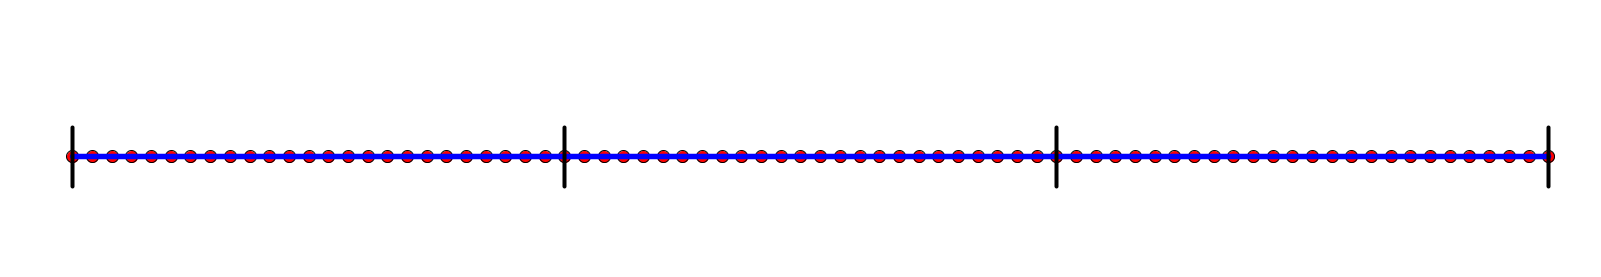
\includegraphics[width=12cm]{../fig/Cap03-EjemploProbabilidadGeometrica01.png}
	\end{enColor}
	\begin{bn}
	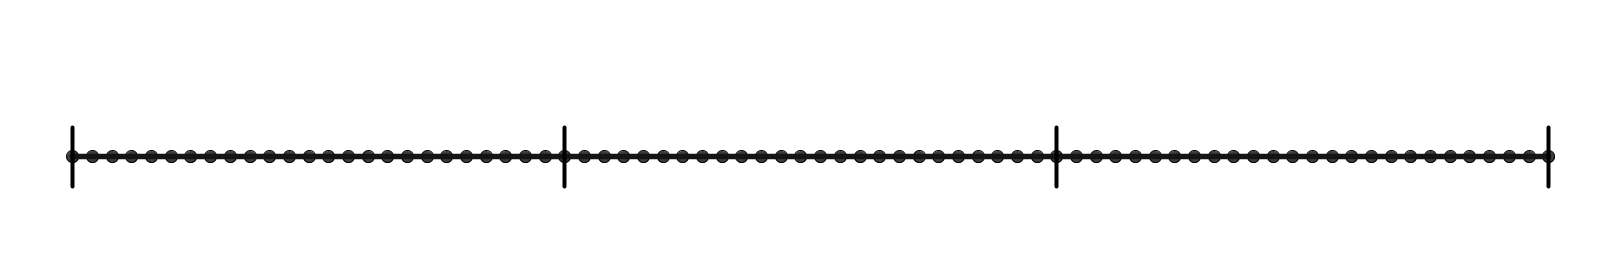
\includegraphics[width=12cm]{../fig/Cap03-EjemploProbabilidadGeometrica01-bn.png}
	\end{bn}
	\caption{Si elegimos uno de esos puntos al azar, ¿cuál es la probabilidad de que pertenezca al
    segmento situado más a la derecha?}
    \label{Cap03:fig:EjemploProbabilidadGeometricaElegirPuntoIntervalo}
    \end{figure}
Aquí sí que podemos usar la regla de Laplace, para concluir que, puesto que (muy aproximadamente) la tercera parte de esos puntos pertenecen al intervalo, la probabilidad que buscamos debe ser $1/3$. Una manera alternativa de pensar en esto, sin recurrir a la regla de Laplace, consiste en pensar que elegimos no ya uno, sino muchos de entre esos $n_0+1$ puntos, y estudiamos la {\em proporción} de puntos que pertenecen al intervalo $[0,1/3]$. Está intuitivamente claro que esa proporción se parecerá mucho a $1/3$. Además, la aproximación a $1/3$ es tanto mejor cuanto mayor sea $n_0$. En el Tutorial03 trataremos de justificar usando el ordenador lo que la intuición nos está diciendo para este caso.

Naturalmente, el problema con el enfoque que hemos usado en este ejemplo es que en el intervalo $[0,1]$ hay infinitos puntos, distintos de esos $n_0$ puntos que hemos seleccionado. Así que, por más grande que sea $n_0$, la lista de puntos que podemos elegir dista mucho de la idea teórica de ``cualquier punto del intervalo [0,1]''. Por eso este procedimiento no resulta del todo satisfactorio desde el punto de vista teórico. Sin embargo, es una idea interesante y que puede ayudar a guiar nuestra intuición. Por eso merece la pena explorarla, como vamos a hacer en otros ejemplos.
\qed
\end{ejemplo}
La pregunta que hemos discutido en este ejemplo es representativa del tipo de problemas que genéricamente se llaman de {\em Probabilidad Geométrica}. En este caso, en el que elegimos puntos de un segmento, se trata de un problema unidimensional.
%Y un
%ejemplo similar: en una circunferencia de radio 1 se eligen dos puntos al azar. ¿Cuál es la
%longitud media de la cuerda de circunferencia que definen? Esta pregunta es un ejemplo del tipo de
%problemas que genéricamente se llaman de {\em Probabilidad Geométrica}. El fichero GeoGebra
%\begin{center}
% \fichero{../datos/Cap03-ProbabilidadGeometrica01.ggb}{Cap03-ProbabilidadGeometrica01.ggb}
%\end{center}
% ilustra este problema. Para ver otro ejemplo famoso, recomendamos
%visitar la página web de construcciones con GeoGebra de Manuel Sada (en la dirección web
%\link{http://docentes.educacion.navarra.es/msadaall/geogebra}{docentes.educacion.navarra.es/msadaall/geogebra/}),
%donde entre otras muchas cosas interesantes, podéis ver una ilustración de varios problemas
%clásicos de la Probabilidad como el {\em Problema de la aguja de Buffon}, o el {\em
%Problema de Monty Hall}, del que ya hemos hablado.
Vamos a ver ahora otro  ejemplo de probabilidad geométrica, en este caso bidimensional, que nos va a ayudar a seguir avanzando, y sobre el que volveremos varias veces más adelante.
\begin{Ejemplo}
\label{Cap03:ejem:ProbabilidadGeometricaMontecarlo}
Supongamos que tenemos un cuadrado de lado 4 y en su interior dibujamos cierta figura $A$. Para fijar ideas, $A$ puede ser un un círculo de radio 1, centrado en el cuadrado, como en la Figura \ref{Cap03:fig:Circulo}.
    \begin{figure}[h]
	\centering
	\begin{enColor}
% 	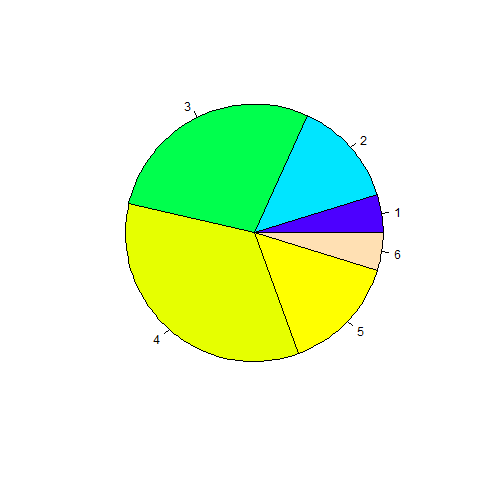
\includegraphics[height=6cm]{../fig/Cap01-DiagramaSectores.png}
% 	\hspace{0.5cm}
	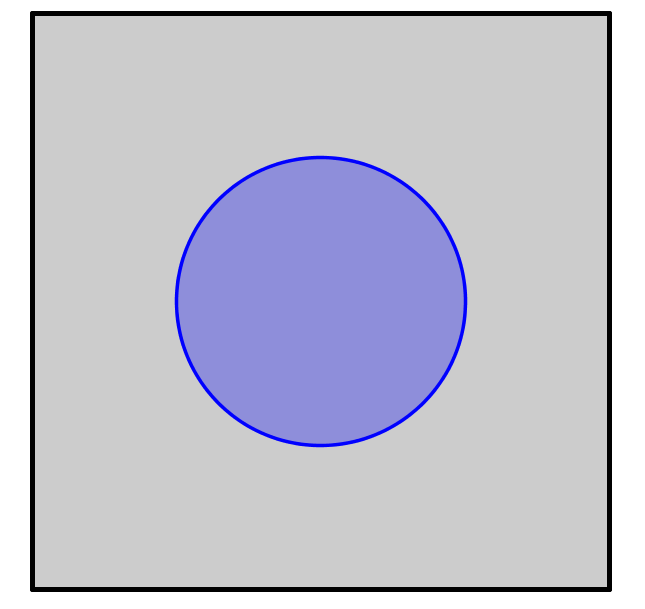
\includegraphics[height=5cm]{../fig/Cap03-Montecarlo.png}
	\end{enColor}
	\begin{bn}
% 	\includegraphics[height=6cm]{../fig/Cap01-DiagramaSectores-bn.png}
% 	\hspace{0.5cm}
	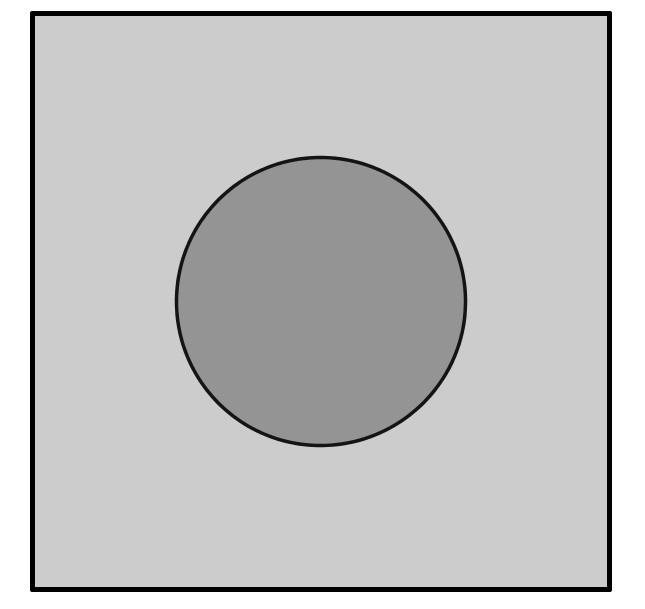
\includegraphics[height=5cm]{../fig/Cap03-Montecarlo-bn.png}
	\end{bn}
	\caption{C\'irculo de radio $1$ centrado en un cuadrado de lado $4$.}\label{Cap03:fig:Circulo}
    \end{figure}
Si tomamos un punto al azar dentro del cuadrado ¿cuál es la probabilidad de que ese punto caiga dentro del círculo $A$?  En el Ejemplo \ref{Cap03:fig:EjemploProbabilidadGeometricaElegirPuntoIntervalo} elegíamos un punto al azar del segmento $[0,1]$, y aquí elegimos un punto al azar en el cuadrado de lado $4$. Una buena manera de pensar en esto es imaginarse que lanzamos un dardo al cuadrado, pero que el lanzamiento es completamente al azar, de manera que  ``todos los puntos del cuadrado son {\em equiprobables}''. Si nos imaginamos que, en lugar de un dardo, lanzamos miles de ellos, ¿qué proporción de esos dardos caerían dentro del círculo (serían {\em favorables} al círculo)? La intuición indica que esa proporción depende del área del círculo. El círculo es la diana, y cuanto más grande sea el área de la diana, más probable será acertar. Esta relación nos permite apreciar una relación entre la idea de probabilidad y la idea de área, que nos resulta mucho más intuitiva. Este vínculo entre área y probabilidad es extremadamente importante. En el Tutorial03 usaremos el ordenador para explorar esta relación más detenidamente.

Hemos entrecomillado la frase anterior sobre la equiprobabilidad de los puntos, porque ahí está el conflicto fundamental que hace que ejemplos como este sean imposibles de reconciliar con la regla de Laplace. En cualquier región del cuadrado hay infinitos puntos. En particular, el círculo contiene infinitos puntos. Si todos esos puntos del círculo tienen la misma probabilidad, distinta de cero, entonces por muy pequeña que sea, aunque sea una billonésima, cuando sumemos un trillón de puntos obtendremos... desde luego, más de uno. Así que no podemos tener estas cosas a la vez:
\begin{enumerate}
    \item los puntos son equiprobables.
    \item su probabilidad es distinta de cero.
    \item la probabilidad es un número entre 0 y 1 que se calcula, como en la regla de Laplace, sumando las probabilidades de los puntos individuales.
\end{enumerate}
Para salir de este atolladero, necesitamos, en ejemplos como este, una forma radicalmente distinta de pensar la probabilidad.
\qed
\end{Ejemplo}
¿Cuál es esa forma distinta de pensar la probabilidad? Los ejemplos anteriores nos dan la clave. Debería quedar claro, al pensar detenidamente sobre estos ejemplos, que la noción de probabilidad y la noción de área de una figura plana tienen muchas propiedades en común (en los problemas unidimensionales, en lugar del área usamos la longitud).  El problema con el que se encontraron los matemáticos, claro está, es que la propia noción teórica de área es igual de complicada de definir que la Probabilidad. Esto puede resultar un poco sorprendente, porque, a diferencia de lo que sucede con la probabilidad, el área resulta una idea intuitiva. De hecho, es engañosamente fácil de entender.
\begin{ejemplo}
\label{cap03:ejem:TrianguloSierpinski}
Para ver un ejemplo en el que la noción de área empieza a resultar resbaladiza, podemos pensar en la construcción del llamado {\em triángulo de Sierpinski}\index{triángulo de Sierpinski} (ver el enlace [\,\ref{enlace0002}\label{enlace0002a}\,]). Este conjunto se construye mediante un proceso iterativo, mediante una serie de operaciones que se repiten ``infinitas veces'' (técnicamente, por un paso al límite). Las primeras etapas de la construcción se ilustran en la Figura \ref{Cap03:fig:TrianguloSierpinski}.
\begin{figure}[b!]
\begin{center}
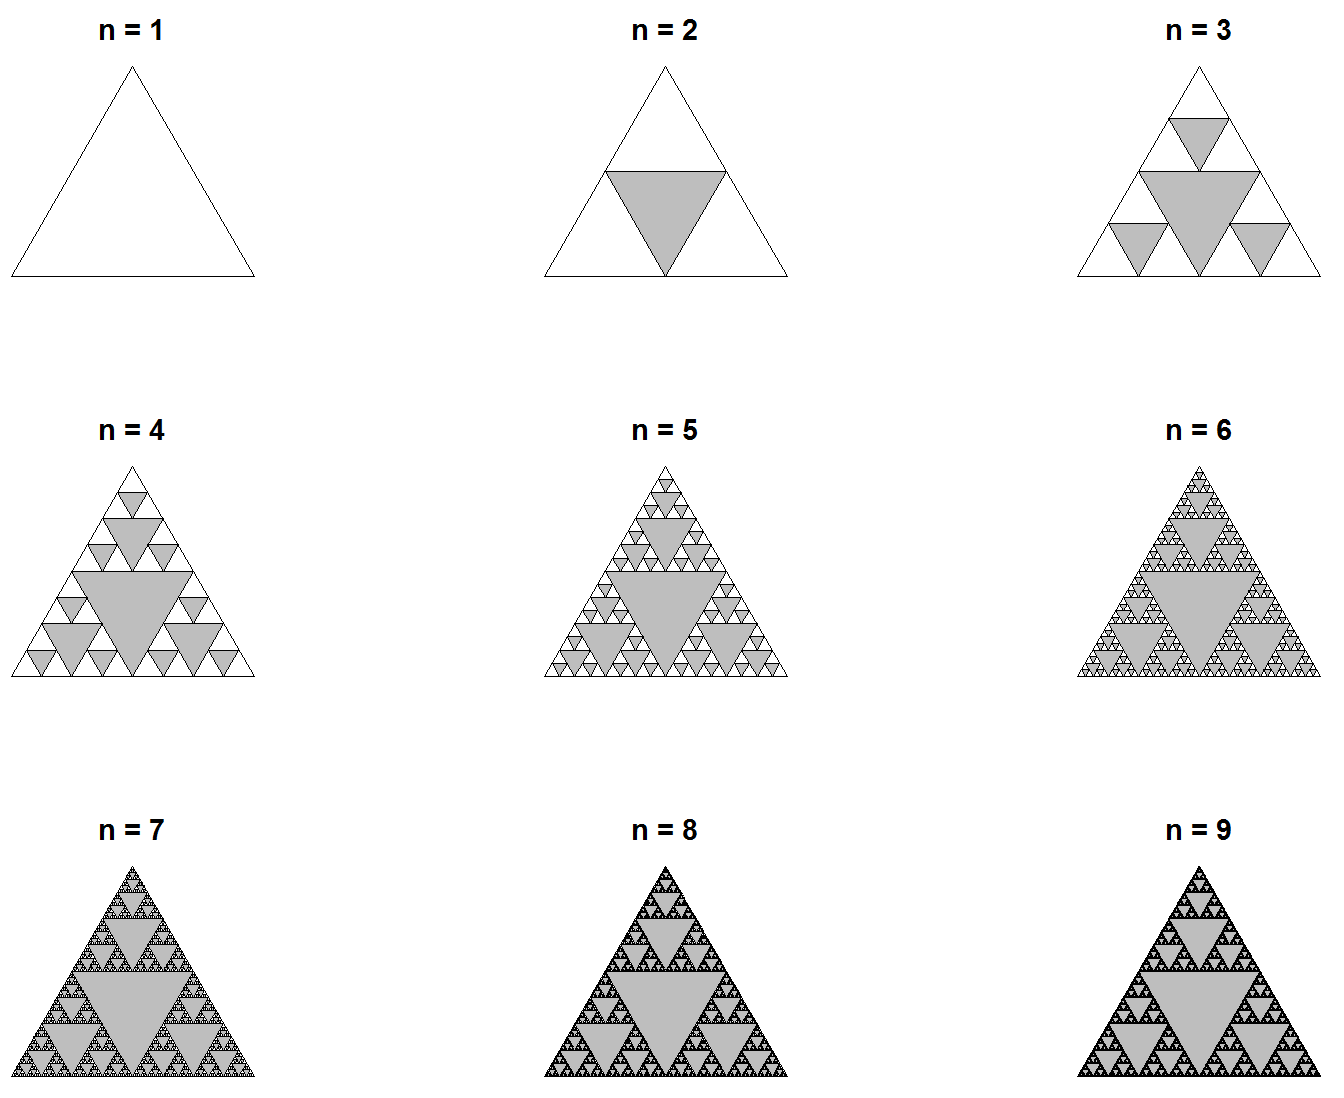
\includegraphics[width=14cm]{../fig/Cap03-SierpinskiConR.png}
\caption{Las primeras etapas en la construcción del triángulo de Sierpinski}
\label{Cap03:fig:TrianguloSierpinski}
\end{center}
\end{figure}
Como se ve en esa figura, el punto de partida ($n=1$) es un triángulo equilátero. Inicialmente consideramos todos los puntos del triángulo (borde e interior). En la siguiente etapa ($n=2$), {\em eliminamos} del conjunto los puntos del triángulo central sombreado, de manera que lo que queda son los tres triángulos equiláteros, copias a escala del original. En el siguiente paso ($n=3$), aplicamos la misma operación (``eliminar el triángulo central'') a cada uno de los triángulos que conservamos en la fase $n=2$. Y así vamos procediendo, aplicando esa misma operación en cada paso para pasar de $n$ a $n+1$. El Triángulo de Sierpinski es el conjunto de puntos que quedan ``al final'' de este proceso. De alguna manera, es un conjunto formado por ``infinitos triángulos infinitamente pequeños''.
\qed
\end{ejemplo}
%\begin{center}
%  \fichero{../datos/Cap03-Sierpinski.ggb}{Cap03-Sierpinski.ggb},
%\end{center}
%que ilustra los primeros pasos en la construcción de la figura llamada {\em el triángulo de Sierpinski}\index{triángulo de Sierpinski}, que se obtiene como límite siguiendo el proceso que ilustra ese fichero.\qed
Los entrecomillados del final de este ejemplo indican que esas son descripciones informales. Y ese es precisamente el problema con el que se encontraron los matemáticos a finales del siglo XIX: no resultaba nada fácil encontrar una manera formal, rigurosa, de definir conceptos como el área para figuras como esta (y otras mucho más complicadas). A causa de estos, y otros problemas similares, los matemáticos de aquella época (y entre ellos, muy destacadamente, Andréi Kolmogórov; más información sobre él en el enlace [\,\ref{enlace0001}\label{enlace0001a}\,])\label{enlace0001a}
construyeron una {\em Teoría Axiomática de la Probabilidad}. Aquí no podemos entrar en todos los
detalles técnicos, que son complicados, pero podemos decir que, esencialmente, se trata de lo siguiente:
    \begin{itemize}
        \item[(A)] Inicialmente tenemos un \index{espacio muestral}{\sf espacio muestral} $\Omega$, que representa el conjunto de todos los posibles resultados de un experimento.
        \item[(B)] Un \index{suceso aleatorio}{\sf suceso aleatorio} es un subconjunto del espacio muestral. Esta es la parte en la que vamos a ser menos rigurosos. En realidad, no todos los subconjuntos sirven, por la misma razón que hemos visto al observar que no es fácil asignar un área a todos los subconjuntos posibles. Pero para entender qué subconjuntos son sucesos y cuáles no, tendríamos que definir el concepto de $\sigma$-álgebra\index{$\sigma$-álgebra}\index{sigma álgebra}, y eso nos llevaría demasiado tiempo. Nos vamos a conformar con decir que hay un {\em tipo especial de subconjuntos}, los sucesos aleatorios, a los que sabemos asignarles una probabilidad.
        \item[(C)] La \index{función Probabilidad}{\sf Función Probabilidad}, que representaremos con una letra $P$,  esuna función o regla que  asigna un cierto número $P(A)$ a cada suceso aleatorio $A$ del espacio muestral $\Omega$. Y esa función probabilidad debe cumplir  tres propiedades, que aparecen más abajo. Antes de enunciarlas, necesitamos una aclaración sobre la notación que aparece en la segunda propiedad  de la probabilidad: el \index{suceso unión}\index{unión}{\sf suceso unión} $A_1\cup A_2$ significa que suceden $A_1$ o $A_2$ (o ambos a la vez). El \index{suceso intersección}\index{intersección}{\sf suceso intersección} $A_1\cap A_2$ significa que $A_1$ y $A_2$ ocurren ambos simultáneamente. A menudo se usan diagramas (de Venn), como el de la Figura \ref{Cap03:fig:DiagramaVennInterseccionSucesos},para representar, conceptualmente, las uniones o intersecciones de sucesos.

\begin{figure}[htbp]
\begin{center}
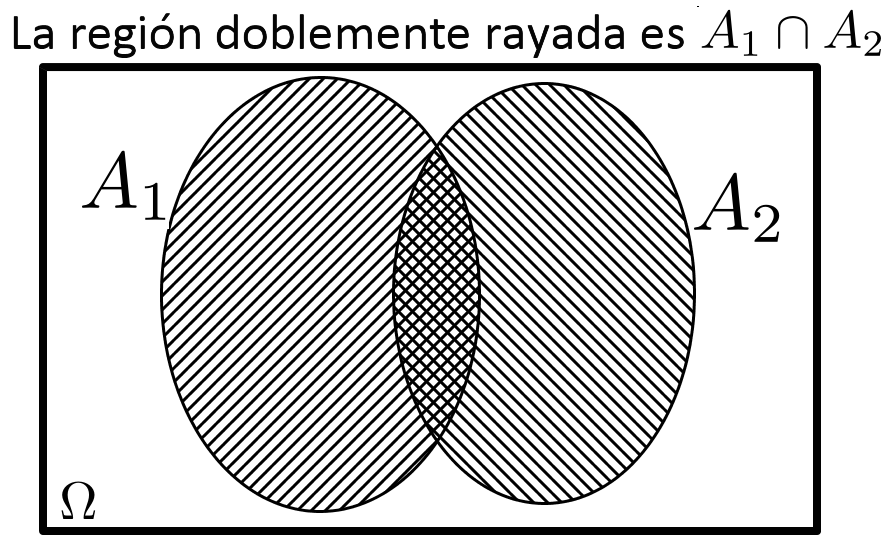
\includegraphics[height=4cm]{../fig/Cap03-DiagramaVennInterseccionSucesos.png}
	\caption{Diagrama para la intersección de dos sucesos }\label{Cap03:fig:DiagramaVennInterseccionSucesos}
\end{center}
\end{figure}

En un diagrama como ese, el rectángulo exterior representa el espacio muestral, y cada una de las figuras rayadas que aparecen, de forma elíptica,  representa un suceso. En este caso, la elipse de la izquierda se corresponde con $A_1$ y la de la derecha con $A_2$. La intersección $A_1\cap A_2$ es la zona común a ambas elipses. En cambio, la unión $A_\cup A_2$ sería la zona total que cubren las dos elipses, conjuntamente.

\pagebreak
\hspace{-0.8cm}Con esa notación, las propiedades de la Probabilidad son estas:

\begin{center}
\fcolorbox{black}{Gris025}{
\begin{minipage}{12cm}
    \centering {\bf Propiedades fundamentales de la Función Probabilidad.}
    \label{cap03:def:PropiedadesFundamentalesFuncionProbabilidad}
    \index{probabilidad, propiedades fundamentales}
    \begin{enumerate}
        \item Sea cual sea el suceso aleatorio $A$, siempre se cumple que $0\leq P(A)\leq 1$.
            \item Si $A_1$ y $A_2$ son \index{sucesos aleatorios disjuntos}\index{disjuntos} sucesos aleatorios disjuntos, es decir si $A_1\cap A_2=\emptyset$ (esto equivale a decir que es imposible que $A_1$ y $A_2$ ocurran a la vez) entonces
                \[P(A_1\cup A_2)=P(A_1)+P(A_2).\]
                En el caso $A_1\cap A_2=\emptyset$ también diremos que los sucesos son {\sf incompatibles}.\index{sucesos incompatibles}\index{incompatibles, sucesos}
            \item La probabilidad del espacio muestral completo es $1$. Es decir, $P(\Omega)=1$.
    \end{enumerate}
\end{minipage}}
\end{center}
    \end{itemize}
La Figura \ref{Cap03:fig:DiagramaVennSucesosDisjuntos} representa, en un diagrama conceptual, el caso de dos sucesos incompatibles (o disjuntos).

\begin{figure}[htbp]
\begin{center}
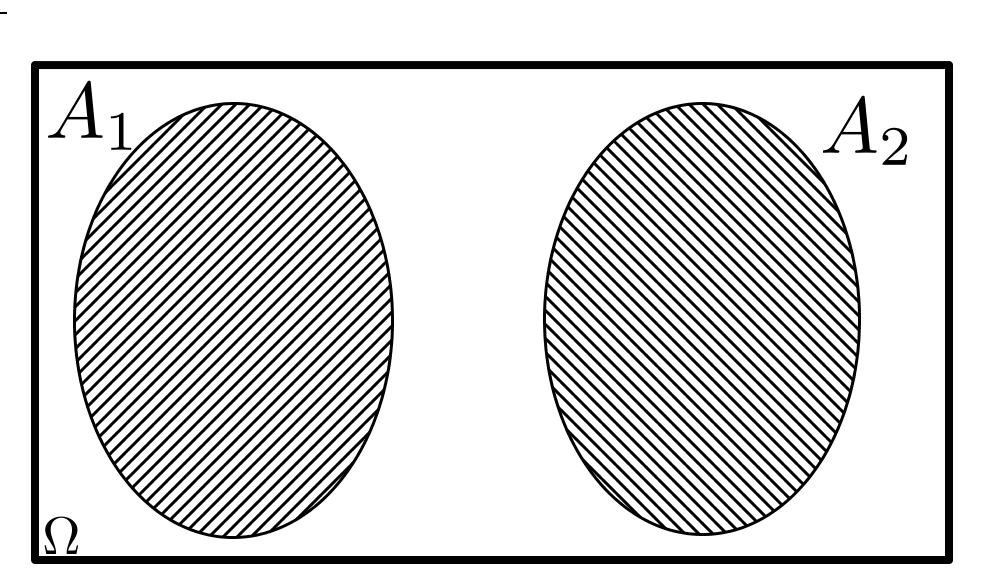
\includegraphics[height=4cm]{../fig/Cap03-DiagramaVennSucesosDisjuntos.png}
	\caption{Dos sucesos incompatibles o disjuntos.}\label{Cap03:fig:DiagramaVennSucesosDisjuntos}
\end{center}
\end{figure}

La forma en la que se asignan o {\sf distribuyen} las probabilidades define el \index{modelo probabilístico}{\sf modelo probabilístico} que utilizamos en cada problema. Por ejemplo, la Regla de Laplace es el modelo probabilístico típico que usamos en situaciones como las de los juegos de azar que hemos descrito, y en general, cuando, basados en nuestra experiencia, podemos suponer la existencia de una familia de sucesos elementales equiprobables. En los problemas de probabilidad geométrica adoptamos, a menudo (pero no siempre), un modelo probabilístico que consiste en suponer que la probabilidad de una región es proporcional a su área. \\

Vamos a ver como se aplican estas ideas al ejemplo del lanzamiento de una moneda hasta la primera cara que vimos antes.
\begin{Ejemplo}[\bf Continuación del Ejemplo \ref{Cap03:ejem:LanzamientoMonedaHastPrimeraCara}, pág. \pageref{Cap03:ejem:LanzamientoMonedaHastPrimeraCara}]\label{cap03:ejem:LanzamientoMonedaHastPrimeraCara:2}

En este caso, podemos definir un modelo de probabilidad así. El espacio muestral $\Omega$ es el conjunto de todas las listas de la forma
\[a_1=\smiley, a_2=\dag\smiley, a_3=\dag \dag\smiley,\ldots,a_k=\hspace{-7pt}\overbrace{\dag \dag \dag \cdots\dag \dag \dag }^{(k-1)\mbox{ cruces }}\hspace{-7pt}\smiley,\ldots\]
es decir, $k-1$ cruces hasta la primera cara. Fíjate en que este espacio muestral tiene infinitos elementos. Todos los subconjuntos se consideran sucesos aleatorios, y para definir la probabilidad decimos que:
\begin{enumerate}
    \item $P(a_k)=P(\overbrace{\dag \dag \dag \cdots\dag \dag \dag }^{k-1\mbox{ cruces }}\hspace{-5pt}\smiley)=\dfrac{1}{2^{k}}$,
    \item Si $A=\{a_i\}$ es un suceso aleatorio, es decir, $A$ es un conjunto de listas de cruces y caras, entonces $P(A)=\sum P(a_i)$. Dicho de otro
modo, la probabilidad de un conjunto de listas es igual a la suma de las probabilidades de las listas que lo forman\footnote{No vamos a entretenernos
en comprobar que, con esta definición, se cumplen las tres propiedades fundamentales, pero le garantizamos al lector que, en efecto, así es.}. Es
decir, que si
        \[A=\{a_1,a_3,a_6\}=\{\smiley,\,\dag \dag\smiley\, ,\, \dag \dag \dag \dag \dag\smiley\,\},\]
        entonces
        \[P(A)=P(a_1)+P(a_3)+P(a_6)=\dfrac{1}{2}+\dfrac{1}{2^3}+\dfrac{1}{2^6}.\]
\end{enumerate}
Ahora podemos calcular la probabilidad de que gane la persona que empieza lanzando. Ese suceso es:
\[A=\{a_1,a_3,a_5,a_7,\ldots\}=\mbox{el primer jugador gana en la $k$-ésima jugada},\]
y por lo tanto su probabilidad es:
\[P(A)=\underbrace{P(a_1)+P(a_3)+P(a_5)+P(a_7)+\cdots}_{\mbox{listas de longitud impar}}=
\dfrac{1}{2}+\dfrac{1}{2^3}+\dfrac{1}{2^5}+\dfrac{1}{2^7}+\cdots=\dfrac{2}{3}.
\]
Esta última suma la hemos calculado usando el hecho de que se trata de la suma de una {\sf progresión geométrica} de razón $\dfrac{1}{2^2}$. No podemos entretenernos en explicar cómo se hacen este tipo de sumas infinitas (series), pero sí queremos tranquilizar al lector, asegurándole que las progresiones geométricas son las más fáciles de todas. En el Tutorial03 veremos cómo se puede usar el ordenador para calcular algunas sumas como estas.\qed
\end{Ejemplo}

Este enfoque también sirve para los problemas-ejemplo de probabilidad geométrica que hemos discutido antes. Esencialmente, lo que hay que tener presente es que la definición de Función Probabilidad está relacionada con el área, y el único matiz importante es que un área puede ser arbitrariamente grande o pequeña (por lo tanto, puede ser cualquier número positivo), mientras que una probabilidad viene obligada a ser un número entre 0 y 1. La forma natural de hacer esto es fijar de antemano cierta figura geométrica $\Omega$, que es el espacio muestral, y definir la probabilidad de un  suceso $A$ como
\[P(A)=\dfrac{\mbox{área de }A}{\mbox{área de }\Omega}.\]
En el Ejemplo \ref{Cap03:ejem:ProbabilidadGeometricaMontecarlo}, la probabilidad de un suceso (subconjunto del cuadrado grande) es igual al área de ese suceso dividida por 16 (el área del cuadrado grande). {\sf Un punto o una recta son sucesos de probabilidad cero} (porque no tienen área). Esta última propiedad resulta un poco chocante a los recién llegados al mundo de la Probabilidad, pero no lo es tanto si se piensa en términos de áreas. {La originalidad (y genialidad) de la idea de Kolmogórov es que se conserva la propiedad de la aditividad de la probabilidad (la propiedad (2)), a cambio de pequeñas ``paradojas'' aparentes, como esta de que los puntos {\em individualmente considerados} tienen todos probabilidad cero, pero el {\em conjunto de (infinitos) puntos} tiene probabilidad no nula. Insistimos, esto sólo parece una paradoja hasta que se piensa en términos de área, y en ese momento nos damos cuenta de que con el área sucede exactamente lo mismo. ¿Qué queda entonces de esa idea de equiprobabilidad ingenua, en la que decíamos que todos los puntos del cuadrado son equiprobables? Lo que queda es una versión al menos igual de intuitiva, pero mucho más coherente: todas las regiones del cuadrado {\em del mismo área} son equiprobables.}

Y una última aclaración: la probabilidad definida mediante la Regla de Laplace cumple, desde luego, las tres propiedades fundamentales que hemos enunciado. Lo que hemos hecho ha sido {\em generalizar} la noción de probabilidad a otros contextos en los que la idea de favorables/posibles no se aplica. Pero los ejemplos que se basan en la Regla de Laplace son a menudo un buen ``laboratorio mental'' para poner a prueba nuestras ideas y nuestra comprensión de las propiedades de las probabilidades.

\subsection{Más propiedades de la Función Probabilidad.}
\label{cap03:subsec:MasPropiedadesFuncionProbabilidad}

Las tres propiedades básicas de la Función Probabilidad tienen una serie de consecuencias que vamos a explorar en el resto de este capítulo. En el Tutorial03 veremos ejemplos y ejercicios que muestran como estas propiedades a menudo permiten convertir un problema complicado de probabilidad en otro más sencillo. Por ejemplo, en lugar de contar los casos favorables a un suceso puede resultar más fácil contar las veces en las que {\em no} ocurre dicho suceso. Así, la pregunta: {\em ¿cuántos números menores que 100 tienen cifras repetidas?} puede convertirse en esta más sencilla: {\em ¿cuántos números menores que 100 no tienen cifras repetidas?} También podemos tratar de descomponer un suceso en trozos más fáciles de contar por separado. Las primeras y más sencillas de esas propiedades aparecen resumidas en este cuadro:	
    \begin{center}
    \fcolorbox{black}{Gris025}{
    \begin{minipage}{12cm}
        \centering {\bf Propiedades adicionales de la Función Probabilidad.}
         \begin{enumerate}
            \item Sea cual sea el suceso aleatorio $A$, si $A^c$ es el
            \index{suceso complementario}\index{complementario} {\sf suceso complementario o suceso contrario}\index{suceso contrario}\index{contrario}
            (es decir ``no ocurre $A$'') siempre se cumple que
            \[P(A^c)=1-P(A).\]
            \item La probabilidad del\index{suceso vacío} {\sf suceso vacío}
            $\emptyset$ es $0$; es decir \[P(\emptyset)=0.\]
            \item Si $A\subset B$, (se lee: si $A$ es un subconjunto de $B$,
            es decir si siempre que ocurre $A$ ocurre $B$), entonces
            \[P(A)\leq P(B)\mbox{, y además }P(B)=P(A)+P(B\cap A^c).\]
            \item Si $A_1$ y $A_2$ son sucesos aleatorios cualesquiera,
            \begin{equation}\label{cap03:ecu:ProbabilidadUnionDosSucesosCasoGeneral}
                P(A_1\cup A_2)=P(A_1)+P(A_2)-P(A_1\cap A_2).
            \end{equation}
        \end{enumerate}
    \end{minipage}}
    \end{center}
La última de estas propiedades se puede generalizar a $n$ sucesos aleatorios. Veamos como queda para tres, y dejamos al lector que imagine el resultado general {\em (ojo a los signos)}:
    \[\begin{array}{l}
    P(A_1\cup A_2\cup A_3)=\\
    =\underbrace{\left(P(A_1)+P(A_2)+P(A_3)\right)}_{\mbox{tomados de 1 en 1}}\colorbox{lightgrey}{\bf -}\underbrace{\left(P(A_1\cap A_2)+P(A_1\cap A_3)+P(A_2\cap A_3)\right)}_{\mbox{tomados de 2 en 2}}\\
    \colorbox{lightgrey}{\bf +}\underbrace{\left(P(A_1\cap A_2\cap A_3)\right)}_{\mbox{tomados de 3 en 3}}.
    \end{array}
    \]
La Figura \ref{Cap03:fig:DiagramaVennUnioTresSucesos} ilustra esta propiedad. Los sucesos intersección dos a dos corresponden a las zonas doblemente rayadas de la figura, y la intersección tres a tres corresponde a la parte central, triplemente rayada.

\begin{figure}[h!]
\begin{center}
    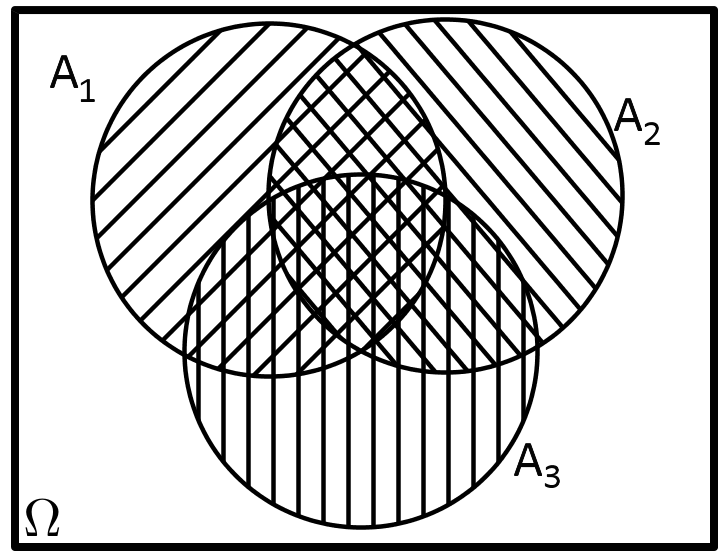
\includegraphics[height=5.5cm]{../fig/Cap03-DiagramaVennUnioTresSucesos.png}
	\caption{Diagrama para la intersección de tres sucesos.}
    \label{Cap03:fig:DiagramaVennUnioTresSucesos}
\end{center}
\end{figure}




\section{Probabilidad condicionada. Sucesos independientes.}
\label{cap03:sec:ProbabilidadCondicionadaIndependencia}


\subsection{Probabilidad condicionada.}
\label{cap03:subsec:ProbabilidadCondicionada}

El concepto de probabilidad condicionada trata de reflejar los cambios en el
valor de la Función Probabilidad que se producen cuando tenemos {\em
información parcial} sobre el resultado de un experimento aleatorio. Para
entenderlo, vamos a usar, como ejemplo, uno de esos casos en los que la Regla
de Laplace es suficiente para calcular probabilidades. Vamos a pensar que, al
lanzar dos dados, nos dicen que la suma de los dados ha sido mayor que 3.
Pero imagina que no sabemos el resultado; puede ser $(1,3), (2,5)$, etc.,
pero no, por ejemplo, $(1,1)$, o $(1,2)$. Con esa información en nuestras
manos, nos piden que calculemos la probabilidad de que la suma de los dos
dados haya sido un $7$. Nuestro cálculo debe ser distinto ahora que sabemos
que el resultado es mayor que 3, porque el número de resultados posibles (el
denominador en la fórmula de Laplace), ha cambiado. Los resultados como
$(1,1)$ o $(2,1)$ no pueden estar en la lista de resultados posibles, {\em si
sabemos que la suma es mayor que $3$}.  {\sf\em La información que tenemos
sobre el resultado cambia nuestra asignación de probabilidades}. Este es un
buen momento para recordar el problema de Monty Hall (y volver a recomendar
al lector que, si no lo hizo, busque el vídeo de la serie Numb3rs del que ya
hemos hablado).

Usando como ``laboratorio de ideas'' la Regla de Laplace, estamos tratando de
definir la {\em probabilidad del suceso $A$, {\sf sabiendo} que ha ocurrido
el suceso $B$}. Esto es lo que vamos a llamar la \index{probabilidad
condicionada} {\sf probabilidad de $A$ condicionada por $B$, y lo
representamos por $P(A|B)$}. Pensemos en cuáles son los cambios en la
aplicación de la Regla de Laplace (favorables/posibles), cuando sabemos que
el suceso $B$ ha ocurrido. Antes que nada recordemos que, si el total de
resultados elementales posibles es $n$ entonces
    \[P(A)=\dfrac{\mbox{núm. de casos favorables a $A$}}{n},\]
y también se cumple
    \[P(B)=\dfrac{\mbox{núm. de casos favorables a $B$}}{n}.\]
Veamos ahora como deberíamos definir $P(A|B)$. Puesto que sabemos que $B$ ha
ocurrido, los casos posibles ya no son todos los $n$ casos posibles
originales: ahora los únicos casos posibles son los que corresponden al
suceso $B$.  ¿Y cuáles son los casos favorables del suceso $A$, una vez que
sabemos que $B$ ha ocurrido? Pues aquellos casos en los que $A$ y $B$ ocurren
simultáneamente (o sea, el suceso $A\cap B$). En una fracción:
    \[P(A|B)=\dfrac{\mbox{número de casos favorables a $A\cap B$}}{\mbox{número de casos favorables a $B$}}.\]
Si sólo estuviéramos interesados en la Regla de Laplace esto sería tal vez
suficiente. Pero, para poder generalizar la fórmula a otras situaciones, como
la Probabilidad Geométrica, hay una manera mejor de escribirlo. Dividimos el
numerador y el denominador por $n$ y tenemos:
    \[P(A|B)=\dfrac{\quad\left(\dfrac{\mbox{número de casos favorables a $A\cap B$}}{n}\right)\quad}{\left(\dfrac{\mbox{número de casos favorables a $B$}}{n}\right)}=\dfrac{P(A\cap B)}{P(B)}.\]
¿Qué tiene de bueno esto? Pues que la expresión que hemos obtenido ya no hace
ninguna referencia a casos favorables o posibles, nos hemos librado de la
Regla de Laplace, y hemos obtenido una expresión general que sólo usa la
Función de Probabilidad (e, insistimos, hacemos esto porque así podremos
usarla, por ejemplo, en problemas de Probabilidad Geométrica). Ya tenemos la
definición:
    \begin{center}
    \fcolorbox{black}{Gris025}{
    \begin{minipage}{12cm}
        \begin{center}{\bf Probabilidad condicionada.}
				        \label{cap03:def:ProbabilidadCondicionada}
				\end{center}
        La probabilidad del suceso $A$ condicionada por el suceso $B$ se define así:
        \[P(A|B)=\dfrac{P(A\cap B)}{P(B)}.\]
        donde se supone que $P(B)\neq 0$.
    \end{minipage}}
    \end{center}
%
%
%
%
%
%        \begin{center}
%        \fbox{\colorbox{Gris025}{\begin{minipage}{14cm}
%        \begin{center}
%%        \vspace{2mm}
%        {\bf Probabilidad condicionada: }
%        \end{center}
%        La probabilidad del suceso $A$ condicionada por el suceso $B$ se define así:
%            \[P(A|B)=\dfrac{P(A\cap B)}{P(B)}.\]
%        donde se supone que $P(B)\neq 0$.
%        \end{minipage}}}
%        \end{center}

Vamos a ver un ejemplo de como calcular estas probabilidades condicionadas, usando de nuevo el lanzamiento de dos dados.
    \begin{Ejemplo}
    \label{Cap03:probabilidadCondicionadaLanzamientoDosDados}
    Se lanzan dos dados. ¿Cuál es la probabilidad de que la diferencia (en valor absoluto) entre los valores de ambos dados (mayor-menor) sea menor que 4, sabiendo que la suma de los dados es 7?\\
    Vamos a considerar los sucesos:
    \begin{itemize}
        \item[S:] La suma de los dados es 7.
        \item[D:] La diferencia en valor absoluto de los dados es menor que 4.
    \end{itemize}
    En este caso es muy fácil calcular $P(D|S)$. Si sabemos que la suma es $7$, los resultados sólo pueden ser $(1,6),(2,5),(3,4),(4,3),(5,2),(6,1)$. Y de estos, sólo $(1,6)$ y $(6,1)$ no cumplen la condición de la diferencia. Así que $P(D|S)=4/6$. Vamos a ver si coincide con lo que predice la fórmula. El suceso $S\cap D$ ocurre cuando ocurren {\sf a la vez} $S$ y $D$. Es decir la suma es 7 {\sf y a la vez} la diferencia es menor que $4$. Es fácil ver que, de los 36 resultados posible, eso sucede en estos cuatro casos: \[(2,5),(3,4),(4,3),(5,2),\]
    por tanto, la probabilidad de la intersección es $P(S\cap D)=\frac{4}{36}$. Y, por otro lado, la probabilidad del suceso $S$ es $P(S)=\frac{6}{36}$ (ver el Ejemplo \ref{Cap03:ejem:CualEsProbabilidadSumaDosDadosIgualASiete} de la pág. \pageref{Cap03:ejem:CualEsProbabilidadSumaDosDadosIgualASiete}; de hecho, hemos descrito los sucesos favorables a $S$ un poco más arriba). Así pues,
    \[P(D|S)=\dfrac{P(D\cap S)}{P(S)}=\dfrac{4/36}{6/36}=\dfrac{4}{6}=\dfrac{2}{3}\approx 0.666\ldots,\]
    como esperábamos. En el Tutorial3 veremos como usar el ordenador para simular este experimento, y comprobar los resultados que predice la teoría.
    \qed
    \end{Ejemplo}
En realidad, la probabilidad condicionada se usa habitualmente para calcular
la probabilidad de una intersección. Este método se basa en la siguiente
reformulación de la definición, llamada {\sf Regla del Producto} para las
probabilidades condicionadas.
        \begin{center}
        \fcolorbox{black}{Gris025}{
        \begin{minipage}{8cm}
        	\vspace{-5mm}
        \begin{equation}\label{cap03:ecu:ReglaProductoProbabilidadCondicionada}
            P(A\cup B) = P(A|B)P(B)=P(B|A)P(A),
        \end{equation}
        \end{minipage}}
        \end{center}
porque la definición de probabilidad condicionada dice que los dos miembros son dos formas de escribir $P(A\cap B)$. Teniendo esto en cuenta, si se conocen las probabilidades de $A$ y $B$, se puede obtener fácilmente una probabilidad condicionada a partir de la otra. Este resultado es extremadamente útil para, por ejemplo, descomponer problemas de probabilidad en varias etapas, y usar las probabilidades condicionadas, normalmente más fáciles de calcular. Veremos ejemplos en el Tutorial03.

\subsubsection{Tablas de contingencia y probabilidad condicionada}
\label{cap03:subsubsec:TablasContingenciaProbabilidadCondicionada}

    La noción de probabilidad condicionada $P(A|B)$ se utiliza a menudo en situaciones en las que la información sobre los sucesos $A$ y $B$ (y sus complementarios $A^c$ y $B^c$) se presenta en forma de tablas, que en este contexto se llaman {\sf tablas de contingencia}\index{tabla de contingencia}. Las tablas de contingencia aparecerán varias veces en el curso, y en el Capítulo \ref{cap:TablasContingenciaTestChi2} hablaremos extensamente sobre ellas. En el próximo ejemplo vamos a ver un caso típico, y clásico, de aplicación del concepto de probabilidad condicionada: las {\sf pruebas diagnósticas}\index{pruebas diagnósticas}\index{diagnósticas, pruebas}, para la detección de una enfermedad.
\begin{ejemplo}
\label{cap03:ejem:PruebasDiagnosticas01}
\index{pruebas diagnósticas}\index{diagnósticas, pruebas}
           Vamos a suponer que analizamos una prueba diagnóstica para cierta enfermedad. Las pruebas diagnósticas no son infalibles. A veces la prueba dará como resultado que una persona padece la enfermedad, cuando en realidad no es así. Es lo que se llama un {\sf falso positivo}\index{falso positivo}. Y en otras ocasiones el problema será el contrario. La prueba dirá que la persona no padece la enfermedad, aunque de hecho la padezca. Eso es un {\sf falso negativo}\index{falso negativo}. Vamos a suponer que sabemos que en una población de 10000 personas, aproximadamente el 2\% están afectados por esa enfermedad. La Tabla \ref{cap03:tabla:ejemploPruebasDiagnosticas}, que es típica de esta clase de situaciones, contiene los valores precisos de este ejemplo.
        \begin{table}[h!]
        \begin{center}
            \begin{tabular}{llccc}
            &&\multicolumn{3}{c}{\underline{\bf Padecen la enfermedad}}\\

                                      &          & Sí &  No & Total\\
            \hline
          \underline{\bf Resultado de la Prueba} & Positivo & 192&  158&   350\\
                                      & Negativo &  4 & 9646&  9650\\
            \hline
                                      & Total    & 196& 9804& 10000\\
            \hline
            \end{tabular}
        \end{center}
        \caption{Tabla de contingencia del Ejemplo \ref{cap03:ejem:PruebasDiagnosticas01}}
        \label{cap03:tabla:ejemploPruebasDiagnosticas}
        \end{table}

        Como puede verse en esa tabla, hay dos {\em familias de sucesos} en las que podemos pensar:
        \begin{itemize}
           \item sano o enfermo.
           \item resultado positivo o negativo de la prueba diagnóstica.
         \end{itemize}
        Estas dos familias de sucesos representan dos formas de dividir o clasificar a la población (en sanos/enfermos por un lado, o en positivos/negativos por otro lado).

        Para calcular la probabilidad de que un individuo esté sano, debemos mirar en el {\em margen inferior} (de otro modo, la última fila de la tabla). Allí vemos que hay 196 personas enfermas de un total de 10000. Por lo tanto, la probabilidad es:
        \[P(\mbox{enfermo})=\dfrac{196}{10000}=0.0196.\]
        Como decíamos antes, aproximadamente un 2\%. Puesto que, en este ejemplo, suponemos que una persona sólo puede estar sana o enferma, la probabilidad de estar enfermo es:
        \[P(\mbox{sano})=1-P(\mbox{enfermo})=1-0.0196=0.9804.\]
        Este resultado también se puede obtener, directamente, del margen inferior de la tabla. Si en lugar de sano/enfermo pensamos en las probabilidades de diagnóstico positivo/negativo, entonces tenemos que mirar en el {\em margen derecho} (la última columna) de la tabla. Allí vemos que, de las 10000 personas, 350 han dado positivo, así que
        \[P(\mbox{positivo})=\dfrac{350}{10000}=0.035.\]
        De la misma forma (o restando de uno) se tiene:
        \[P(\mbox{negativo})=\dfrac{9650}{10000}=0.965.\]
        Con esto vemos que los márgenes de la tabla (inferior y derecho) nos permiten obtener las probabilidades de las dos familias de sucesos que intervienen en este ejemplo. ¿Qué significado tienen, en términos de probabilidades, los cuatro valores {\em interiores de la tabla} (los que ocupan las dos primeras filas y columnas)? Por ejemplo, ¿qué representa el valor 4 de la segunda fila, primera columna? Se trata del número de personas que, a la vez, padecen la enfermedad y han dado negativo en el diagnóstico. Por lo tanto ese número se refiere al suceso intersección
        \[\mbox{enfermo}\cap\mbox{negativo},\]
        y su probabilidad es:
        \[P\left(\mbox{enfermo}\cap\mbox{negativo}\right)=\dfrac{4}{10000}=0.0004\]
        De la misma forma, para los otro tres valores:
        \[
        \begin{cases}
        P\left(\mbox{enfermo}\cap\mbox{positivo}\right)=\dfrac{192}{10000}=0.0192\\[5mm]
        P\left(\mbox{sano}\cap\mbox{positivo}\right)=\dfrac{158}{10000}=0.0158\\[5mm]
        P\left(\mbox{sano}\cap\mbox{negativo}\right)=\dfrac{9646}{10000}=0.9646
        \end{cases}
        \]
        ¿Y las probabilidades condicionadas? Esas probabilidades no se ven directamente en una tabla como la Tabla \ref{cap03:tabla:ejemploPruebasDiagnosticas}. Pero podemos obtenerlas fácilmente, operando por filas o por columnas, según se trate. Por ejemplo, para calcular
        \[P\left(\mbox{negativo} | \mbox{enfermo} \right),\]
        puesto que sabemos que el individuo está enfermo, tenemos que limitarnos a considerar los $196$ individuos de la primera columna. De esos, la segunda fila nos informa de que sólo $4$ han dado negativo en la prueba, lo cual significa que:
        \[P\left(\mbox{negativo} | \mbox{enfermo} \right)=\dfrac{4}{196}\approx 0.02.\]
        Es decir, que hay sólo un 2\% de falsos negativos. De la misma forma:
        \[P\left(\mbox{positivo} | \mbox{sano} \right)=\dfrac{158}{9804}\approx 0.016,\]
        demuestra que la prueba tiene también una tasa muy baja de falsos positivos. Estos dos resultados nos hacen pensar que la prueba diagnóstica es muy buena, así que cuando un paciente recibe un diagnóstico positivo, lo normal es que piense que hay una probabilidad muy alta de estar enfermo. Pero ¿cuál es, realmente, esa probabilidad? Tenemos que calcular
        \[P\left(\mbox{enfermo} | \mbox{positivo}\right),\]
        y ahora, puesto que sabemos que el individuo ha dado positivo, tenemos que limitarnos a considerar los $350$ individuos de la primera fila. De esos, la primera columna nos dice que $192$ están, de hecho enfermos. Así que la probabilidad que buscamos es:
        \[P\left(\mbox{enfermo} | \mbox{positivo}\right)=\dfrac{192}{350}\approx 0.5486.\]
        Apenas un 55\%. ¿Cómo es posible, si la prueba parecía ser tan buena? La explicación, y es esencial mirar atentamente la Tabla \ref{cap03:tabla:ejemploPruebasDiagnosticas} para entenderla, es que realmente hay muy pocas personas enfermas, sobre el total de la población. Así que los falsos positivos, que se calculan sobre una gran cantidad de personas sanas, representan una fracción muy importante del total de positivos.
        \qed
      \end{ejemplo}
      Después de ver este ejemplo,  puede ser un buen momento para que el lector, si no la conoce, escuche la charla TED de Peter Donnelly (ver el enlace [\,\ref{enlace0007}\,]\label{enlace0007a}), titulada {\em ``How juries are fooled by statistics''} (``La Estadística engaña a los jurados''; hay subtítulos en español o inglés). La charla trata sobre Probabilidad, Estadística, y el papel que juegan en terrenos tan variados como la Genética, o los procesos judiciales.

      La Tabla \ref{cap03:tabla:ejemploPruebasDiagnosticas} es, como hemos dicho, un ejemplo de una {\sf tabla de contingencia}. En este caso es una tabla $2\times 2$, pero veremos más adelante (en el Capítulo \ref{cap:TablasContingenciaTestChi2}) otros ejemplos en los que se hace necesario contemplar tablas de contingencia de dimensiones distintas.


\subsection{Sucesos independientes.}
\label{cap03:subsec:SucesosIndependientes}

¿Qué significado debería tener la frase {\em ``el suceso $A$ es independiente del suceso $B$''}\,? Parece evidente que, si los sucesos son independientes, el hecho de saber que el suceso $B$ ha ocurrido no debería afectar para nada a nuestro cálculo de la probabilidad de que ocurra $A$. Esta idea tiene una traducción inmediata en el lenguaje de la probabilidad condicionada, que es de hecho la definición de sucesos independientes:
        \begin{center}
        \fcolorbox{black}{Gris025}{
        \begin{minipage}{12cm}
            \begin{center}
            	{\bf Sucesos independientes.}
            \end{center}
            Los sucesos $A$ y $B$ son \index{sucesos independientes}{\sf sucesos independientes}\index{independientes, sucesos} si
                \[P(A|B)=P(A).\]
            Esto es equivalente a decir que:
            \begin{equation}\label{cap03:ecu:ReglaProductoProbabilidadDosSucesosIndependientes}
                P(A\cap B)=P(A)P(B).
            \end{equation}
            Esta propiedad se conoce como la {\sf Regla del Producto para sucesos independientes.}\index{regla del producto para sucesos independientes}\index{sucesos independientes, regla del producto}.  En particular, {\bf cuando los sucesos $A$ y $B$ son independientes}, se cumple:
            \[P(A\cup B)=P(A)+P(B)-P(A)P(B).\]
        \end{minipage}}
        \end{center}
En general los sucesos $A_1,\ldots,A_k$ son independientes cuando para {\em cualquier colección} que tomemos de ellos, la probabilidad de la intersección es el producto de las probabilidades. Eso significa que, en particular, sucede
    \begin{equation}\label{cap03:ecu:ReglaProductoProbabilidad_N_SucesosIndependientes}
        P(A_1\cap A_2\cap\cdots\cap A_k)=P(A_1) \cdot P(A_2)\cdot\cdots\cdot P(A_k).\mbox{ {!`}{!`}Para sucesos independientes!!}
    \end{equation}
Pero insistimos, la independencia significa que esto debe cumplirse para cualquier subcolección. Por ejemplo,  para que $A_1,\ldots,A_5$ sean independientes, debe cumplirse
\[P(A_1\cap A_2\cap A_4)=P(A_1)\cdot P(A_2)\cdot P(A_4),\]
pero también
\[P(A_1\cap A_5)=P(A_1)\cdot P(A_5),\]
entre otras muchas. ¿Cuántas? Es un buen ejercicio de Combinatoria convencerse de que son $2^k - k -1$, donde $k$ es el número de sucesos. {!`}Verificar la independencia de una colección de sucesos puede ser muy complicado! Normalmente partiremos de situaciones en las que sabemos {\em a priori} que se cumple la independencias, y entonces usaremos estas propiedades para poder calcular las probabilidades de las intersecciones que nos interesen.

\subsubsection{Sucesos independientes y sucesos disjuntos (incompatibles).}

A menudo, al principio, hay cierta confusión entre la noción de sucesos independientes y la de sucesos disjuntos, que también hemos llamado incompatibles. Tal vez sea el origen de la confusión tenga algo que ver con el parecido entre esas dos palabras.  En cualquier caso, recordemos que dos sucesos son disjuntos si no pueden ocurrir a la vez (ver Figura \ref{Cap03:fig:DiagramaVennSucesosDisjuntos}, pág. \pageref{Cap03:fig:DiagramaVennSucesosDisjuntos}). Por ejemplo, si $A$ es el suceso {\em ``Hoy es lunes''} y $B$ es el suceso {\em ``Hoy es viernes''}, está
claro que $A$ y $B$ no pueden ocurrir a la vez. Por otra parte, los sucesos son independientes cuando uno de ellos no aporta ninguna información sobre
el otro. Y volviendo al ejemplo, en cuanto sabemos que hoy es lunes (ha ocurrido $A$), ya estamos seguros de que no es viernes (no ha ocurrido $B$).
Así que la información sobre el suceso $A$ nos permite decir algo sobre el suceso $B$, y eso significa que no hay independencia.
        \begin{center}
        \fcolorbox{black}{Gris025}{
        \begin{minipage}{7cm}
                        {\sf Dos sucesos disjuntos nunca son independientes.}
        \end{minipage}}
        \end{center}

\section{Probabilidades totales y Teorema de Bayes.}
\label{cap03:sec:ProbabilidadesTotalesReglaBayes}


\subsection{La regla de las probabilidades totales. Problemas de urnas.}
\label{cap03:subsec:ProbabilidadesTotales}


El resultado que vamos a ver utiliza la noción de probabilidad condicionada para calcular la probabilidad de un suceso $A$ mediante la estrategia de {\em divide y vencerás}.  Se trata de descomponer el espacio muestral completo en una serie de sucesos $B_1,\ldots,B_k$ que reunan estas características:\\[3mm]
\begin{minipage}{6.5cm}
    \begin{enumerate}
    	\item[(1)] $\Omega=B_1\cup B_2\cup\cdots\cup B_k.$
    	%\textcolor{red}{Es decir, cada suceso elemental est\'an en alguno de los $B_i$.}
    	\item[(2)] $B_i\cap B_j=\emptyset$, para cualquier par $i\neq j$.
    	%\textcolor{red}{ning\'un suceso suceso elemental est\'a repetido.}
    	\item[(3)] $P(B_i)\neq 0$ para $i=1,\ldots,k$.
    	%\textcolor{red}{Todos los sucesos $B_i$ son posibles.}
    \end{enumerate}
\end{minipage}
\begin{minipage}{6.5cm}
	\qquad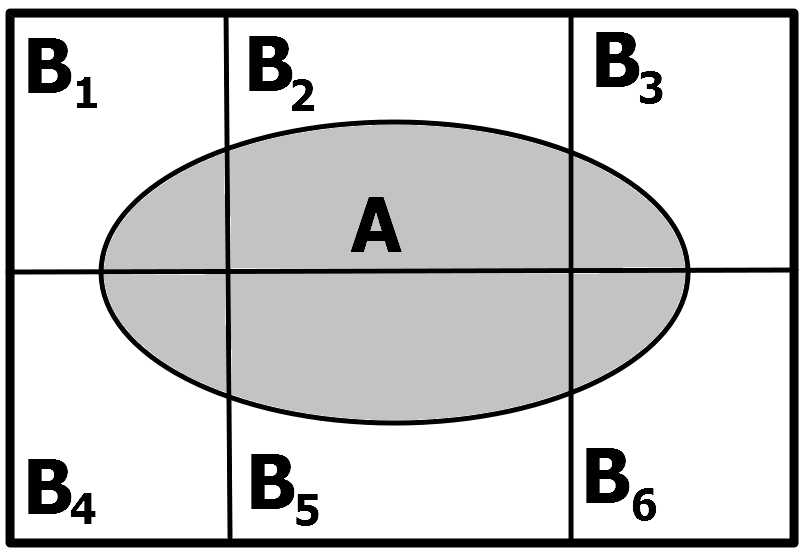
\includegraphics[height=2.5cm]{../fig/Cap03-ProbabilidadesTotales.png}
\end{minipage}
\\[3mm]	
{En tal caso decimos que $B_1,\ldots,B_k$ constituyen una partici\'on (1) disjunta (2) del espacio muestral. \index{partici\'on disjunta del espacio muestral}} Entonces (ver la figura) podemos usarlos para calcular $P(A)$ usando la :
        \begin{center}
        \fcolorbox{black}{Gris025}{
        \begin{minipage}{12cm}
            \begin{center}
						\bf Regla de las probabilidades totales.\index{regla de las probabilidades totales}
						\end{center}
            Si los sucesos $B_1,\ldots,B_K$ cumplen las condiciones (1), (2) y (3) entonces:
            \[P(A)=P(B_1)P(A|B_1)+P(B_2)P(A|B_2)+\cdots+P(B_k)P(A|B_k).\]
        \end{minipage}}
        \end{center}
Esta expresión permite calcular la probabilidad de $A$ cuando conocemos de antemano las probabilidades de los sucesos $B_1,\ldots,B_k$ y es fácil calcular las probabilidades condicionadas $P(A|B_i)$. Si los sucesos $B_i$ se han elegido bien, la información de que el suceso $B_i$ ha ocurrido puede en ocasiones simplificar mucho el cálculo de $P(A|B_i)$.

El método de las probabilidades totales se usa sobre todo cuando conocemos varias vías o mecanismos por los que el suceso $A$ puede llegar a producirse. El ejemplo clásico son los {\sf problemas de urnas}, que sirven de prototipo para muchas otras situaciones.
    \begin{Ejemplo}
    \label{cap03:ejem:ProbailidadTotalEjemploUrnas}
        Supongamos que tenemos dos urnas, la primera con 3 bolas blancas y dos negras, y la segunda con 4 bolas blancas y 1 negra. Para extraer una bola lanzamos un dado. Si el resultado es $1$ o $2$ usamos la primera urna; si es cualquier otro número usamos la segunda urna. ¿cuál es la probabilidad de obtener una bola blanca?\\
        Llamemos $A$ al suceso {\em ``ha salido una bola blanca''} ,  $B_1$ al suceso {\em ``se ha usado la primera urna''}, y $B_2$ al suceso {\em ``se ha usado la segunda urna''}. Entonces,de la regla de Laplace obtenemos $P(B_1)=\frac{1}{3}$, $P(B_2)=\frac{2}{3}$. Y ahora, cuando sabemos que $B_1$ ha ocurrido (es decir, que estamos usando la primera urna), es fácil calcular $P(A|B_1)$.  Se trata de la probabilidad de extraer una bola blanca de la primera urna: $P(A|B_1)=\frac{3}{5}.$ De la misma forma $P(A|B_2)=\frac{4}{5}$. Con todos estos datos, el Teorema de las Probabilidades Totales da como resultado:
        \[P(A)=P(B_1)P(A|B_1)+P(B_2)P(A|B_2)=
        \dfrac{1}{3}\cdot\dfrac{3}{5}+\dfrac{2}{3}\cdot\dfrac{4}{5}=\dfrac{11}{15}.\]
        En el Tutorial-03 usaremos el ordenador para verificar, mediante una simulación, estos resultados.
    \qed
    \end{Ejemplo}
Este ejemplo, con dados y bolas, puede parecer artificioso, y alejado de las aplicaciones prácticas. Pero piensa en esta situación: si tenemos una fábrica que produce la misma pieza con dos máquinas distintas, y sabemos la proporción de piezas defectuosas que produce cada una de las máquinas, podemos identificar máquinas con urnas y piezas con bolas, y vemos que el método de las probabilidades totales nos permite saber cuál es la probabilidad de que una pieza producida en esa fábrica sea defectuosa. De la misma forma, si sabemos la probabilidad de desarrollar cáncer de pulmón, en  fumadores y no fumadores, y sabemos la proporción de fumadores y no fumadores que hay en la población total, podemos identificar cada uno de esos tipos de individuos (fumadores y no fumadores) con una urna, y el hecho de desarrollar o no cáncer con bola blanca o bola negra. Como puede verse, el rango de aplicaciones de este resultado es bastante mayor de lo que parecía a primera vista.


\subsection{Teorema de Bayes. La probabilidad de las causas.}
\label{cap03:subsec:TeoremaBayesProbabilidadCausas}



La regla de las probabilidades totales puede describirse así: si conocemos varios mecanismos posibles (los sucesos $B_1,\ldots,B_k$) que dan como resultado el suceso $A$, y las probabilidades asociadas con esos mecanismos, ¿cuál es la probabilidad de ocurra el suceso $A$? El Teorema de Bayes le da la vuelta a la situación. Ahora suponemos que el suceso $A$ {\em de hecho ha ocurrido}.  Y, puesto que puede haber ocurrido a través de distintos mecanismos, nos podemos preguntar ¿cómo de probable es que el suceso $A$ haya ocurrido a través de, por ejemplo, el primer mecanismo $B_1$? Insistimos, no vamos a preguntarnos por la probabilidad del suceso $A$, puesto que suponemos que ha ocurrido. Nos preguntamos por la probabilidad de cada una de los mecanismos o causas que conducen al resultado $A$. Por eso a veces el Teorema de Bayes se describe como un resultado sobre la probabilidad de las causas.

¿Cómo podemos conseguir esto? La pregunta se puede formular así: sabiendo que el suceso $A$ ha ocurrido, ¿cuál es la probabilidad de que haya ocurrido a través del mecanismo $B_i$? De otra manera: sabiendo que el suceso $A$ ha ocurrido, ¿cuál es la probabilidad de que eso se deba a que $B_i$ ha ocurrido? Es decir, queremos averiguar el valor de
    \[P(B_i|A)\mbox{\quad para i=1,\ldots,k}.\]
Quizá lo más importante es entender que, para calcular este valor, {\em la información de la que disponemos es exactamente la misma que en el caso de las probabilidades totales}. Es decir, conocemos los valores $P(B_1),\ldots,P(B_k)$ y las probabilidades condicionadas $P(A|B_1),\ldots,P(A|B_k)$, {!`}qué son justo al revés de lo que ahora queremos!.

Y la forma de conseguir el resultado es esta. Usando que:
    \[P(A|B_k)P(B_k)=P(A\cap B_k)=\colorbox{lightgrey}{$P(B_k|A)$}P(A),\]
despejamos de aquí lo que queremos, y usamos el teorema de las probabilidades totales de una forma astuta, obteniendo:
\begin{center}
    \fcolorbox{black}{Gris025}{
    \begin{minipage}{13cm}
        \begin{center}
				\bf Teorema de Bayes.\index{teorema de Bayes}
				\end{center}
        Si los sucesos $B_1,\ldots,B_k$ cumplen las condiciones (1), (2) y (3) (ver la Sección \ref{cap03:subsec:ProbabilidadesTotales}), entonces para cualquier $j$ de $1$ a $k$ se tiene:
        {\small
        \[P(B_j|A)=\dfrac{P(B_k)P(A|B_k)}{P(A)} = \dfrac{P(B_k)P(A|B_k)}{P(B_1)P(A|B_1)+P(B_2)P(A|B_2)+\cdots+P(B_k)P(A|B_k)}.\]
        }
    \end{minipage}}
    \end{center}
Obsérvese que:
    \begin{enumerate}
    \item Los valores que necesitamos para calcular esta fracción aparecen en la fórmula de las probabilidades totales.
    \item El numerador es uno de los sumandos del denominador.
    \item Las probabilidades condicionadas de la fracción son justo al revés que las del miembro izquierdo.
    \item El denominador es la probabilidad $P(A)$, calculada a través del teorema de las probabilidades totales.
    \end{enumerate}
Con estas observaciones, la fórmula de Bayes es bastante fácil de recordar. Vamos a ver dos ejemplos de este teorema, ambos relacionados con ejemplos anteriores de este capítulo.
El primero es el ejemplo prototípico, un problema de urnas, que sólo tiene el interés de que nos sirve como modelo mental de la forma en que se aplica el teorema.
\begin{Ejemplo}
    {\bf Continuación del Ejemplo \ref{cap03:ejem:ProbailidadTotalEjemploUrnas}, pág. \pageref{cap03:ejem:ProbailidadTotalEjemploUrnas}}\label{cap03:ejem:EjemploUrnasBayes}. 
    Recordemos que, en aquel ejemplo, teníamos dos urnas. La primera con 3 bolas blancas y dos negras, y la segunda con 4 bolas blancas y 1 negra. Para extraer una bola, se lanza un dado. Si el resultado es $1$ o $2$ usamos la primera urna; si es cualquier otro número usamos la segunda urna.
    Supongamos que hemos hecho ese proceso, y la bola extraída es blanca. ¿Cuál es la probabilidad de que proceda de la primera urna?

    Según nuestra experiencia, los ejercicios del Teorema de Bayes se encuentran entre los que más dificultades causan a los novatos, en cursos como este. Así que vamos a tomarnos este ejemplo con calma, y vamos a detallar minuciosamente, paso a paso, cómo lo abordamos.

    Cuando nos enfrentamos a un problema como este, es crucial aprender a procesar la información del enunciado de forma adecuada. En primer lugar, hay que reconocer una situación como la que hemos descrito, con dos familias {\em básicas} $A$ y $B$ de fenómenos (no importa cuál es $A$ y cuál es $B$). En este ejemplo:
    \begin{enumerate}
    \item Familia $A$: $A_1$ es ``bola blanca'' y $A_2$ es ``bola negra''.
    \item Familia $B$: $B_1$ es ``urna 1'' y $B_2$ es ``urna 2''. (Es lo mismo que $B_1$ es ``dado de dos para abajo'' y $B_2$ es ``dado de tres para arriba'').
    \end{enumerate}
    Un par de observaciones sobre esta notación: en el Ejemplo \ref{cap03:ejem:ProbailidadTotalEjemploUrnas} no hemos distinguido entre suceso $A_1$ y suceso $A_2$. En parte porque se nos preguntaba directamente por una bola blanca, y en parte porque la pregunta era más sencilla. Pero aquí nos conviene ser muy cuidadosos con la notación. Y también es cierto que podríamos decir que $A$ es ``bola blanca'', y $A^c$ es ``bola negra''. Pero nos encontraremos más adelante con muchos ejemplos de problemas de Bayes que son, por así decirlo, multicolores. Cuando encontremos un problema con bolas blancas, negras, rojas, azules, etc., no tendremos más remedio que usar $A_1, A_2, A_3,\ldots$

    Insistimos en que, en este primer paso, las dos familias de sucesos deben ser básicas, en el sentido de muy sencillas de describir. Uno de los errores más comunes que vemos cometer a los principiantes, es elegir un suceso como:
    ``Sale una bola blanca de la urna 1''
    y llamarlo $A_1$. Hay que evitar estas mezclas de ``urnas con bolas'', si no queremos perdernos por el camino.

    Cuando tenemos claro cuáles son las dos familias de sucesos $A$ y $B$ que vamos a usar, podemos empezar a traducir la información del enunciado a probabilidades. Hay que estar atentos, porque en un ejercicio del Teorema de Bayes, {\sf siempre} suceden estas tres cosas:
    \begin{enumerate}
        \item Se nos pide que calculemos una probabilidad condicionada. A menudo lo más fácil es empezar por lo que suele ser el final del enunciado, la pregunta. Y a partir de ahí, una vez entendido lo que nos preguntan, y traducido a probabilidades, volver hacia atrás y ver cuál es la información que nos han dado en el enunciado.\\
            En este ejemplo la pregunta dice ``...hemos hecho ese proceso, y la bola extraída es blanca. ¿Cuál es la probabilidad de que proceda de la primera urna?'' Recordamos que nos preguntan por una probabilidad condicionada, y vemos que es la probabilidad de que se haya usado la urna 1. Así que ya sabemos que, con la elección de nombres que hemos hecho antes, la pregunta es de la forma:
            \[P(B_1\,|\,?\,).\]
            ¿Cuál es el suceso que condiciona? Es decir, ¿cuál es el que debe aparecer a la derecha de la barra en esta probabilidad condicionada? Para saberlo, tenemos que recordar que esa probabilidad condicionada se puede leer ``probabilidad de $B_1$ sabiendo que ha sucedido...''. Y ahora, volvemos a la pregunta buscando algo que el enunciado {\sf nos garantiza que ha sucedido}. La clave es el principio de la frase ``...hemos hecho ese proceso, y la bola extraída es blanca.'' Este enunciado asegura que, de hecho, ha ocurrido el suceso $A_1$ ``la bola es blanca''. Así que lo pide este ejercicio es que calculemos
            \[P(B_1 | A_1).\]
        \item Muchas personas, tras localizar lo que pide el enunciado, escriben directamente la fórmula de Bayes que se necesita. Que, en este ejemplo sería:
            \[P(B_1 | A_1)=\dfrac{P(A_1 | B_1)\cdot P(B_1)}{P(A_1 | B_1)\cdot P(B_1)+P(A_1 | B_2)\cdot P(B_2)}.\]
            Nosotros invitamos al lector a que, sobre todo hasta que haya ganado en experiencia, tenga un poco de paciencia, y que analice y reúna la información que ofrece el resultado, {\sf antes} de escribir la fórmula. Es una cuestión puramente táctica: cuando tenemos la fórmula delante, la tentación de encajar los valores del enunciado en los ``huecos'' que ofrece la fórmula, a menudo nos hace precipitarnos y cometer errores. La habilidad con los ejercicios del Teorema de Bayes se adquiere mediante la familiaridad  con la fórmula, y una buena dosis de experencia interpretando enunciados.

        \item El enunciado contiene información sobre probabilidades condicionadas, del tipo contrario a la que debemos calcular.\\
            En este ejemplo, puesto que tenemos que calcular $P(B_1 | A_1)$, el enunciado nos dará información sobre probabilidades de la forma $P(A_i|B_j)$. Concretamente, esas probabilidades son ``probabilidad de que la bola sea de tal color, sabiendo que procede de tal urna''.  Son justo el tipo de probabilidades que calculábamos en el Ejemplo \ref{cap03:ejem:ProbailidadTotalEjemploUrnas}. Y tenemos esa misma información, así que podemos calcular cualquiera de las probabilidades $P(A_1|B_1)$, $P(A_1|B_2)$, $P(A_2|B_1)$ o $P(A_2|B_2)$. Necesitaremos concretamente $P(A_1 | B_1)$ y $P(A_1 | B_2)$ (aparecen en el numerador de la fórmula de Bayes), que, usando la composición de las urnas, son:
            \[
            \begin{cases}
                P(A_1 | B_1)=\dfrac{3}{5}& \mbox{(bola blanca, urna 1)}.\\[5mm]
                P(A_1 | B_2)=\dfrac{4}{5}& \mbox{(bola blanca, urna 2)}.
            \end{cases}
            \]

        \item Además, el enunciado siempre contiene información sobre probabilidades no condicionadas. De hecho, puesto que tenemos que calcular $P(B_1|A_1)$, el enunciado nos dará probabilidad sobre sucesos de la familia $B$ (la que aparezca a la izquierda de la barra vertical).\\
            En este ejemplo, los sucesos $B_1$ y $B_2$ identifican cuál es la urna que se ha usado. Y eso se determina, como explica el enunciado, lanzando un dado y viendo si el resultado es 1 o 2 (urna 1), o si es alguno de los restantes números (urna 2). Así que, teniendo en cuenta las instrucciones del enunciado, tenemos:
            \[P(B_1)=\dfrac{2}{6}, \quad P(B_2)=\dfrac{4}{6}.\]

    \end{enumerate}
    Con estos tres ingredientes, ya estamos listos para completar la cuenta. Sustituimos los valores necesarios en la fórmula:
            \[P(B_1 | A_1)=\dfrac{P(A_1 | B_1)\cdot P(B_1)}{P(A_1 | B_1)\cdot P(B_1)+P(A_1 | B_2)\cdot P(B_2)}=\dfrac{\dfrac{3}{5}\cdot \dfrac{2}{6}}{\dfrac{3}{5}\cdot \dfrac{2}{6}+\dfrac{4}{5}\cdot\dfrac{4}{6}}=\dfrac{3}{11}.\]
    Proponemos al lector, como ejercicio (que ahora debería ser fácil), que calcule la probabilidad de que la bola proceda de la urna 2, sabiendo que ha resultado ser negra. \qed
\end{Ejemplo}

En el siguiente ejemplo vamos a aplicar las mismas técnicas de análisis del enunciado al caso de las pruebas diagnósticas, en las que el Teorema de Bayes juega un papel especialmente importante.
\begin{ejemplo}
\label{cap03:ejem:PruebasDiagnosticasBayes}
    \index{pruebas diagnósticas}\index{diagnósticas, pruebas}
    Vamos a utilizar los mismos datos que en el Ejemplo \ref{cap03:ejem:PruebasDiagnosticas01}, en el que teníamos toda la información en forma de tabla de contingencia, (ver la Tabla \ref{cap03:tabla:ejemploPruebasDiagnosticas}, pág. \pageref{cap03:tabla:ejemploPruebasDiagnosticas}). En aquel ejemplo calculábamos, a partir de la Tabla, varias probabilidades condicionadas. Concretamente, obtuvimos:
    \[P\left(\mbox{negativo} | \mbox{enfermo} \right)=\dfrac{4}{196}\approx 0.02.\]
    y también:
    \[P\left(\mbox{positivo} | \mbox{sano} \right)=\dfrac{158}{9804}\approx 0.016.\]
    De la primera de ellas se deduce que:
    \[P\left(\mbox{positivo} | \mbox{enfermo} \right)=
    1-P\left(\mbox{negativo} | \mbox{enfermo} \right)=
    1-\dfrac{4}{196}\approx 0.9796.\]
    Vamos a usar estas probabilidades condicionadas, junto con los valores (que también calculamos en aquel ejemplo):
    \[
    \begin{cases}
    P(\mbox{enfermo})=\dfrac{196}{10000}=0.0196,\\[3mm]
    P(\mbox{sano})=\dfrac{9804}{10000}=0.9804,
    \end{cases}
    \]
    para calcular una de las probabilidades recíprocas. Concretamente, calcularemos:
    \[P\left(\mbox{enfermo} | \mbox{positivo}\right).\]
    En el Ejemplo \ref{cap03:ejem:PruebasDiagnosticas01} ya obtuvimos este valor directamente, pero aquí vamos a usar el Teorema de Bayes para llegar a ese resultado. Se tiene:
    {\small
    \[P\left(\mbox{enfermo} | \mbox{positivo}\right)=
    \dfrac{P\left(\mbox{positivo} | \mbox{enfermo}\right)\cdot P(\mbox{enfermo})}
    {P\left(\mbox{positivo} | \mbox{enfermo}\right)\cdot P(\mbox{enfermo})+
    P\left(\mbox{positivo} | \mbox{sano}\right)\cdot P(\mbox{sano})}.
    \]
    }
    Es decir, sustituyendo los valores:
    \[P\left(\mbox{enfermo} | \mbox{positivo}\right)={\small
    \dfrac{\left(\dfrac{192}{196}\cdot\dfrac{196}{10000}\right)}{
    \left(\dfrac{192}{196}\cdot\dfrac{196}{10000}\right)+
    \left(\dfrac{158}{9804}\cdot\dfrac{9804}{10000}\right)
    }}\approx 0.5486,
    \]
    que es, naturalmente, el mismo valor que obtuvimos entonces.
%
%       Vamos a suponer que analizamos una prueba diagnóstica para cierta enfermedad. Las pruebas diagnósticas no son infalibles. A veces la prueba dará como resultado que una persona padece la enfermedad, cuando en realidad no es así. Es lo que se llama un {\sf falso positivo}\index{falso positivo}. Y en otras ocasiones el problema será el contrario. La prueba dirá que la persona no padece la enfermedad, aunque de hecho la padezca. Eso es un {\sf falso negativo}\index{falso negativo}. Vamos a suponer que sabemos en una población de 10000, aproximadamente, el 2\% están afectados por esa enfermedad. La Tabla \ref{cap03:tabla:ejemploPruebasDiagnosticas}, que es típica de esta clase de situaciones, contiene los valores precisos de este ejemplo.
%
%    Como puede verse en esa tabla, hay dos {\em familias de sucesos} en las que podemos pensar:
%    \begin{itemize}
%       \item sano o enfermo.
%       \item diagnóstico positivo o negativo.
%     \end{itemize}
%    Estas dos familias de sucesos representan dos formas de dividir o clasificar a la población (en sanos/enfermos por un lado, o en positivos/negativos por otro lado).
%
%    Para calcular la probabilidad de que un individuo esté sano, debemos mirar en el {\em margen inferior} (de otro modo, la última fila de la tabla). Allí vemos que hay 196 personas enfermas de un total de 10000. Por lo tanto, la probabilidad es:
%    \[P(\mbox{sano})=\dfrac{196}{10000}=0.0196.\]
%    Como decíamos antes, aproximadamente un 2\%. Puesto que, en este ejemplo, suponemos que una persona sólo puede estar sana o enferma, la probabilidad de enfermo es:
%    \[P(\mbox{enfermo})=1-P(\mbox{sano})=1-0.0196=0.9804.\]
%    Este resultado también se puede obtener, directamente, del margen inferior de la tabla. Si en lugar de sano/enfermo pensamos en las probabilidades de diagnóstico positivo/negativo, entonces tenemos que mirar en el {\em margen derecho} (la última columna) de la tabla. Allí vemos que, de las 10000 personas, 441 han dado positivo, así que
%    \[P(\mbox{positivo})=\dfrac{350}{10000}=0.035.\]
%    De la misma forma (o restando de uno) se tiene:
%    \[P(\mbox{negativo})=\dfrac{509}{10000}=0.965.\]
%    Con esto vemos que los márgenes de la tabla (inferior y derecho) nos permiten obtener las probabilidades de las dos familias de sucesos que intervienen en este ejemplo. ¿Qué significado tienen, en términos de probabilidades, los cuatro valores {\em interiores de la tabla} (los que ocupan las dos primeras filas y columnas)? Por ejemplo, ¿qué representa el valor 4 de la segunda fila, primera columna? Se trata del número de personas que, a la vez,padecen la enfermedad y han dado negativo en el diagnóstico. Por lo tanto ese número se refiere al suceso intersección
%    \[\mbox{enfermo}\cap\mbox{negativo},\]
%    y su probabilidad es:
%    \[P\left(\mbox{enfermo}\cap\mbox{negativo}\right)=\dfrac{4}{10000}=0.0004\]
%    De la misma forma, para los otro tres valores:
%    \[
%    \begin{cases}
%    P\left(\mbox{enfermo}\cap\mbox{positivo}\right)=\dfrac{192}{10000}=0.0192\\[5mm]
%    P\left(\mbox{sano}\cap\mbox{positivo}\right)=\dfrac{158}{10000}=0.0158\\[5mm]
%    P\left(\mbox{sano}\cap\mbox{negativo}\right)=\dfrac{9646}{10000}=0.9646
%    \end{cases}
%    \]
%    ¿Y las probabilidades condicionadas? Esas probabilidades no se ven directamente en una tabla como la Tabla \ref{cap03:tabla:ejemploPruebasDiagnosticas}. Pero podemos obtenerlas fácilmente, operando por filas o por columnas, según se trate. Por ejemplo, para calcular
%    \[P\left(\mbox{negativo} | \mbox{enfermo} \right),\]
%    puesto que sabemos que el individuo está enfermo, tenemos que limitarnos a considerar los $196$ individuos de la primera columna. De esos, la segunda fila nos informa de que sólo $4$ han dado negativo en la prueba, lo cual significa que:
%    \[P\left(\mbox{negativo} | \mbox{enfermo} \right)=\dfrac{4}{196}\approx 0.02.\]
%    Es decir, que hay sólo un 2\% de falsos negativos. De la misma forma:
%    \[P\left(\mbox{positivo} | \mbox{sano} \right)=\dfrac{158}{9804}\approx 0.016,\]
%    demuestra que la prueba tiene también una tasa muy baja de falsos positivos. Estos dos resultados nos hacen pensar que la prueba diagnóstica es muy buena, así que cuando un paciente recibe un diagnóstico positivo, lo normal es que piense que hay una probabilidad muy alta de estar enfermo. Pero ¿cuál es, realmente, esa probabilidad? Tenemos que calcular
%    \[P\left(\mbox{enfermo} | \mbox{positivo}\right),\]
%    y ahora, puesto que sabemos que el individuo ha dado positivo, tenemos que limitarnos a considerar los $350$ individuos de la primera fila. De esos, la primera columna nos dice que $192$ están, de hecho enfermos. Así que la probabilidad que buscamos es:
%    \[P\left(\mbox{enfermo} | \mbox{positivo}\right)=\dfrac{192}{350}\approx 0.5486.\]
%    Apenas un 56\%. ¿Cómo es posible, si la prueba parecía ser tan buena? La explicación, y es esencial mirar atentamente la Tabla \ref{cap03:tabla:ejemploPruebasDiagnosticas} para entenderla, es que realmente hay muy pocas personas enfermas, sobre el total de la población. Así que los falsos positivos, que se calculan sobre una gran cantidad de personas sanas, representan una fracción muy importante del total de positivos.
    \qed
\end{ejemplo}
Volveremos sobre el tema de las pruebas diagnósticas y su relación con el Teorema de Bayes en la Sección \ref{cap03:sec:OddsPruebasDiagnosticas} (opcional).

\section{Combinatoria: maneras de contar.}
\label{cap03:sec:Combinatoria}
\noindent{\bf Opcional: esta sección puede omitirse en una primera lectura.}\\

La Combinatoria es una parte de las matemáticas que estudia técnicas de recuento. En particular, estudia las posibles formas de seleccionar listas o
subconjuntos de elementos de un conjunto dado siguiendo ciertos criterios (ordenados o no, con repetición o no, etcétera). Por esa razón es de mucha
utilidad para el cálculo de probabilidades, sobre todo cuando se combina con la Regla de Laplace. La Combinatoria, no obstante, puede ser muy
complicada, y en este curso vamos a concentrarnos en los resultados que necesitamos. En particular, como hemos dicho, esta sección puede considerarse como opcional en una primera lectura. Y recurrir a ella como un formulario cuando sea necesario para hacer los ejercicios de Probabilidad. En algún momento, no
obstante, y desde luego antes de llegar al Capítulo \ref{cap:TeoremaCentralLimite}, es esencial haber aprendido el significado de los números
combinatorios, lo cual implica leer al menos hasta la Sección \ref{cap03:subsec:NumerosCombinatorios}.

\begin{itemize}
\item Nos vamos a entretener un poco en deducir alguna de las fórmulas;
de esta forma no tendrás necesidad de memorizarlas.
\item Una forma de abordar estos problemas (y muchos otros) consiste
en considerar casos particulares que contengan los elementos esenciales
y jugar con ellos hasta resolverlos. Despu\'es, extender ese razonamiento a la situaci\'on general.
%Es decir, ni muy sencillos, ni tan complejos como el problema general: representativos)
\item Otra idea interesante es la de trabajar por analog\'ia o asociaci\'on:
\textquestiondown se parece este problema a alguno que ya sé resolver? Para eso,
es muy \'util tener una imagen mental que sirva para reconocer el problema.
Lo veremos enseguida.
\end{itemize}

Un comentario adicional sobre terminología: en Combinatoria es esencial saber si se tiene en cuenta el orden de los elementos de un conjunto, o no.
Para diferenciar esto, cuando hablemos de {\sf listas (o vectores)}\index{lista vs conjunto} siempre daremos por sentado que los elementos están
ordenados, mientras que si hablamos de conjuntos o subconjuntos\index{conjunto vs lista} se sobrentiende que el orden no importa.

Y, antes de meternos en faena, queremos recordarle al lector que tenemos, aún pendientes, los dos experimentos (a) y (b) del apartado \ref{PrimerasNocionesProbabilidad} (pág. \pageref{PrimerasNocionesProbabilidad}). Esta sección proporciona todas las herramientas necesarias para obtener la respuesta en ambos casos. Así que dejamos al lector encargado de la tarea de encontrar la respuesta. La solución, al final de esta Sección.


\subsection{Permutaciones.}
\label{cap03:subsec:Permutaciones}

El problema que abordamos es el siguiente: dado un conjunto de $n$ elementos distintos, \textquestiondown de cu\'antas formas diferentes puedo ordenar
sus elementos? Diremos que cada una de esas ordenaciones es una \index{permutaci\'on} {\sf permutaci\'on} de los elementos del conjunto original.
Atacaremos esto a trav\'es del siguiente ejemplo:
    \begin{Ejemplo} Consideramos cuatro personas y nos preguntamos
	de cu\'antas formas diferentes pueden hacer cola para (digamos) sacar una entrada.
	\begin{itemize}
		\item Para empezar, vamos a poner nombre a los elementos del problema, y a fijarnos en
        los rasgos que lo caracterizan:
		\begin{itemize}
			\item Etiquetamos a las personas con las letras $a,\,b,\,c,\,d$.
            \item La posición que ocupan es importante (no es lo mismo ser el primero que el \'ultimo).
            \item Usaremos todos los elementos del conjunto (las personas).
            \item Cada persona aparece una \'unica vez.
		\end{itemize}
    	Vamos a construir un diagrama para ayudarnos a razonar:
	
        \item En principio, cualquiera de ellas puede ocupar el primer lugar, por lo que tenemos cuatro candidatos a ocupar el primer lugar en la cola, como muestra la Figura \ref{cap03:fig:arbol1}
        	\begin{center}
            \begin{figure}[h!]	
            
\includegraphics[width=13cm]{../fig/Cap03-Permutaciones41.png}
            \caption{Posibles primeros puestos.}\label{cap03:fig:arbol1}
            \end{figure}
            \end{center}
	
        \item Una vez que hemos fijado la primera persona de la cola, hay 3 candidatos a ocupar el segundo lugar (ver Figura \ref{cap03:fig:arbol2}). Es decir, para cada elecci\'on del primer puesto (hay $4$ diferentes) tenemos 3 posibles candidatos para el segundo.
        	\begin{center}
            \begin{figure}[h!]	
            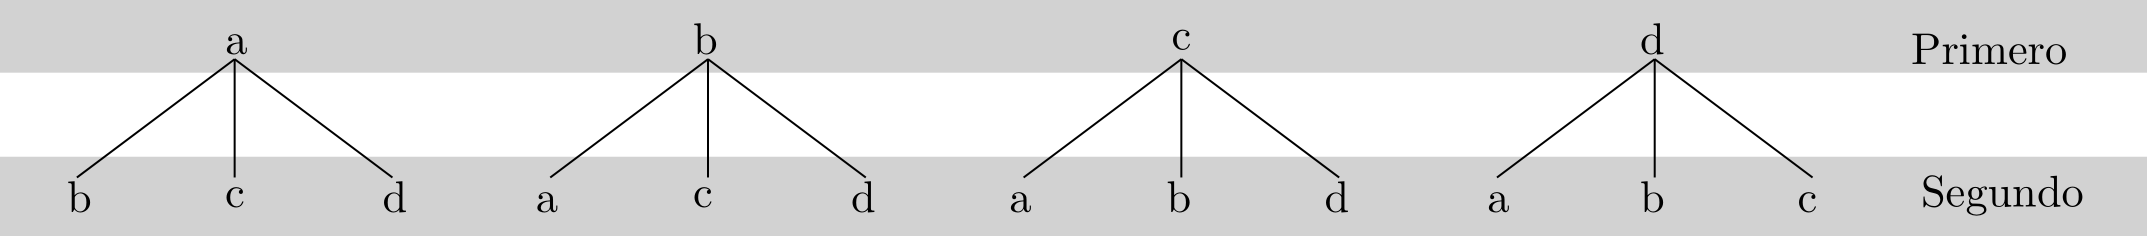
\includegraphics[width=13cm]{../fig/Cap03-Permutaciones42.png}
            \caption{Posibles primer y segundo puestos.}\label{cap03:fig:arbol2}
            \end{figure}
            \end{center}
        \item Es decir, de momento hemos contado $3+3+3+3=4\cdot 3$ casos diferentes.
            \begin{center}
            \begin{figure}[h!]	
            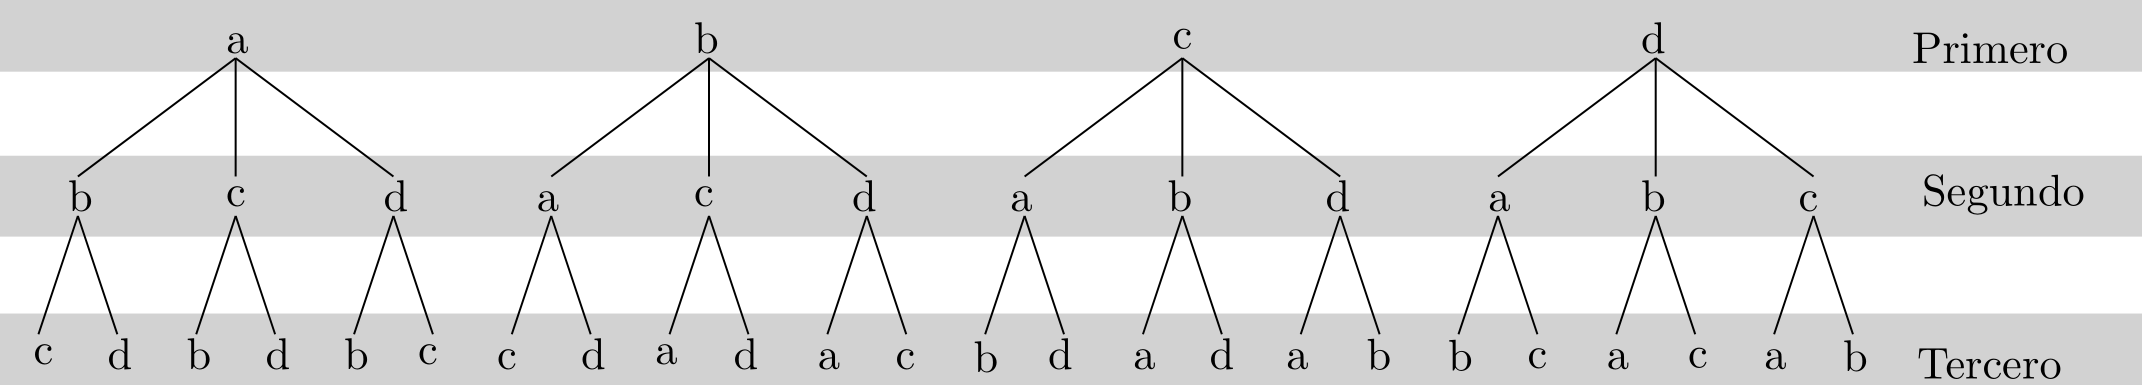
\includegraphics[width=13cm]{../fig/Cap03-Permutaciones43.png}
            \caption{Posibles tres primeros puestos.}\label{cap03:fig:arbol3}
            \end{figure}
            \end{center}
        \item Para la tercera posici\'on, y para cada uno de los casos del paso anterior, s\'olo podemos elegir a una de las dos personas que quedan. Por tanto, tenemos $4\cdot 3\cdot 2$ posibles colas diferentes, las que se muestran en la Figura \ref{cap03:fig:arbol3}. ¿Ves la forma del \'arbol (en las Figuras \ref{cap03:fig:arbol2} y \ref{cap03:fig:arbol3}?
        \item Para la \'ultima posici\'on s\'olo queda una persona: de hecho, no tenemos elección y obtenemos, en total, $4\cdot 3\cdot 2\cdot 1$ posibles colas distintas (Figura \ref{cap03:fig:arbol4}).
    		\begin{center}
            \begin{figure}[h!]	
            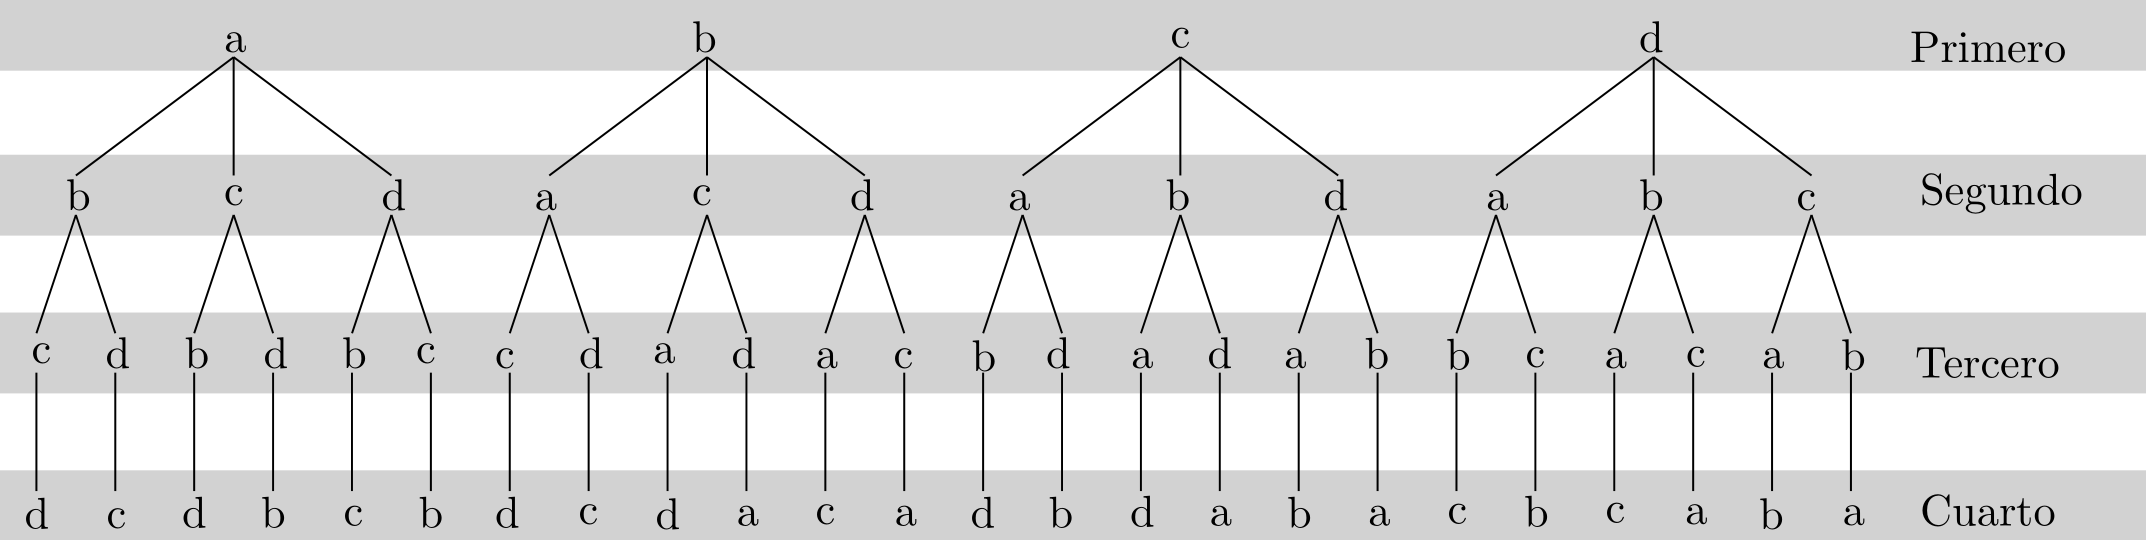
\includegraphics[width=13cm]{../fig/Cap03-Permutaciones44.png}
            \caption{Posibles colas}\label{cap03:fig:arbol4}
            \end{figure}
            \end{center}
    \end{itemize}
    En resumen, hay\, $24=4\cdot 3\cdot 2\cdot 1$ colas distintas posibles con cuatro personas.\qed
    \end{Ejemplo}
Si has entendido lo anterior, verás que no es dif\'icil extender el razonamiento a una cola con un n\'umero {\em arbitrario} de individuos. Para expresar el número de permutaciones de $n$ elementos es muy \'util el concepto de {\sf factorial}\index{factorial}.
    \begin{center}
    \fcolorbox{black}{Gris025}{
    \begin{minipage}{8cm}
        {\begin{center}\bf El factorial de $n=1,2,3,\ldots$.
				\end{center}}
            \[n!=n\cdot(n-1)\cdot(n-2)\cdot\,\ldots\,\cdot3\cdot 2\cdot 1.\]
    \end{minipage}}
    \end{center}
Es decir, el producto de todos los números entre $1$ y $n$. Por ejemplo,
\[10!=10\cdot 9\cdot 8\cdot 7\cdot 6\cdot 5\cdot 4\cdot 3\cdot 2\cdot 1=3628800.\]
(Con diez personas, hay más de tres millones de colas distintas posibles). Además definimos el factorial de $0$ como un caso especial:
    \begin{center}
    \fcolorbox{black}{Gris025}{
    \begin{minipage}{1.5cm}
    \begin{center}
    	$0!=1.$
   \end{center}		
    \end{minipage}}
    \end{center}
La propiedad más llamativa del factorial es su crecimiento extremadamente rápido. Por ejemplo, $100!$ es del orden de $10^{57}$. Este comportamiento
está detrás del fenómeno que se conoce habitualmente como {\sf explosión combinatoria}\index{explosión combinatoria}, en el que empezamos con pocos
elementos, pero al estudiar las listas o subconjuntos formados a partir de esos elementos, los problemas se vuelven rápidamente intratables por su tamaño.

En resumen, el número de permutaciones de $n$ elementos, esto es, el n\'umero de {\sf distintas formas de ordenar} los elementos de un conjunto de $n$ elementos viene dado por
    \begin{center}
    \fcolorbox{black}{Gris025}{
    \begin{minipage}{8cm}
        {\begin{center}\bf Permutaciones de $n$ elementos.
				\end{center}}
            \[\operatorname{Per}(n)=n!=n\cdot(n-1)\cdot(n-2)\cdot\,\ldots\,\cdot3\cdot 2\cdot 1.\]
    \end{minipage}}
    \end{center}


\subsection{Variaciones.}
\label{cap03:subsec:variaciones}

El problema que abordaremos a continuación est\'a muy relacionado con las permutaciones.
Dado un conjunto de $n$ elementos distintos, queremos saber el número de subconjuntos ordenados que podemos hacer con $k$ de sus elementos, donde $0<k<n$. Empezamos con un ejemplo:

\begin{Ejemplo} En una carrera en la que participan $7$ corredores,
de cu\'antas formas posibles pueden repartirse los $3$ primeros puestos?
Recapitulemos:
\begin{itemize}
	\item De nuevo el orden es importante (no es lo mismo ser el primero
		que el tercero).
	\item Ahora NO usaremos todos los elementos (participantes).
	\item Cada corredor, l\'ogicamente, puede aparecer como mucho una vez entre los tres mejores.
\end{itemize}
El razonamiento es esencialmente an\'alogo al que nos llev\'o a deducir la
f\'ormula para las permutaciones. La diferencia es que ahora nos detendremos
en el tercer ``nivel'', puesto que s\'olo nos interesan los tres primeros puestos.
En total hay $7\cdot 6 \cdot 5 =210$ posibles podios.\qed
\end{Ejemplo}
Vamos a poner nombre a estas listas ordenadas: diremos que cada una de ellas es una
{ \sf variaci\'on de $7$ elementos tomados de $3$ en $3$}.

En el lenguaje de los n\'umeros factoriales, podemos expresar esto así. El número de variaciones de $7$ elementos, tomados de $3$ en $3$ es
    	\[\operatorname{V}(7,3)=7\cdot\cdot 6 \cdot 5=\dfrac{7!}{(7-3)!}.\]
Merece la pena detenerse unas lineas en la \'ultima igualdad,
que analizaremos a través de un ejemplo:
\[\begin{array}{rl}
\operatorname{V}(7,4)=7\cdot 6\cdot 5 & =
\dfrac{7 \cdot 6 \cdot 5 \cdot 4 \cdot \cdots \cdot 2 \cdot 1}{4 \cdot \cdots \cdot 2 \cdot 1}\\
	& \\
	& =\dfrac{7!}{(7-3)!}\\
\end{array}
\]
Si leemos esta ecuación de izquierda a derecha, lo que hemos hecho ha sido multiplicar y dividir por la misma cantidad, hasta completar el factorial de $7$ en el numerador. %Si vamos de derecha a izquierda, el mecanismo ha sido el de simplificar algunos factores del numerador con (todos) los del denominador.
%
%{\bf Sin repetici\'on} Listas de $k$ elementos entre $n$ posibles, sin repetir
%elementos y considerando distintas dos listas si el orden de los elementos es distinto.
%\fobox{\operatorname{V}(n,k)=n\cdot(n-1)\cdot\dots\cdot(n-k+1)=\dfrac{n!}{(n-k)!}}
Lo interesante de este truco es que nos permite escribir el caso general de una forma muy compacta:
    \begin{center}
    \fcolorbox{black}{Gris025}{
    \begin{minipage}{10cm}
        {\begin{center} \bf Variaciones de $n$ elementos, tomados de $k$ en $k$.
				\end{center}}
            \[\operatorname{V}(n,k)=n\cdot(n-1)\cdot\dots\cdot(n-k+1)=\dfrac{n!}{(n-k)!}.\]
    \end{minipage}}
    \end{center}
%
%	 \begin{center}
%        \fbox{\colorbox{Gris025}{
%        \begin{minipage}{9cm}
%        		 \begin{center}
%        {\bf Variaciones de $n$ elementos, tomados de $k$ en $k$
%        \index{Variaciones de $n$ elementos, tomados de $k$ en $k$}}%\\[3mm]
%        		 \end{center}
%		\[\operatorname{V}(n,k)=n\cdot(n-1)\cdot\dots\cdot(n-k+1)=\dfrac{n!}{(n-k)!}.\]
%       \end{minipage}}
%        }
%    \end{center}
Para intentar aclarar la relación entre ambos conceptos, podemos ver las permutaciones de $n$ elementos como un caso particular de las variaciones, en el que tomamos $k=n$ elementos.

\subsection{Combinaciones.}
\label{cap03:subsec:Combinaciones}

Tanto en las permutaciones como en las variaciones, el orden en que aparecen los elementos es
importante. Ahora vamos a olvidarnos de \'el. Esta situación recuerda a juegos de apuestas como las de la
{\em Loter\'ia Primitiva} en España (descrita en detalle en el enlace [\,\ref{enlace0008}\,]\label{enlace0008a}). En este tipo de juegos da igual el orden en el que salgan los n\'umeros, lo importante es que coincidan con nuestra apuesta.
	
Estamos interesados en este problema. Dado un conjunto de $n$ elementos
    \[A=\{x_1,x_2,\ldots,x_n\}\]
y un número $k$ con $0\leq k\leq n$, ¿cuántos {\sf subconjuntos distintos} de $k$ elementos podemos formar con los elementos de $A$? Es muy importante entender que, como ya hemos anunciado, al usar la palabra \index{subconjunto}{\sf subconjunto}, estamos diciendo que:
    \begin{enumerate}
        \item el {\sf orden de los elementos es irrelevante}. El subconjunto $\{x_1,x_2,x_3\}$ es el mismo que el subconjunto $\{x_3,x_1,x_2\}$.
        \item los elementos del subconjunto {\sf no se repiten}. El subconjunto $\{x_1,x_2,x_2\}$ es, de hecho, igual al subconjunto $\{x_1,x_2\}$ (y nunca lo escribiríamos de la primera manera, si estamos hablando de subconjuntos).
    \end{enumerate}
Vamos a ponerle un nombre a lo queremos calcular: el número de subconjuntos posibles es el número de   \index{combinaciones de $n$ elementos, tomados de $k$ en $k$}{\sf combinaciones de $n$ elementos, tomados de $k$ en $k$} (cada uno de los subconjuntos es una combinación). Para hacer este c\'alculo, volvamos un momento sobre las variaciones de $n$ elementos, tomados de $k$ en $k$.
Esto no deber\'ia sorprendernos (y no digo que lo haga) porque en ambos casos tenemos un total de $n$ elementos y hacemos subgrupos con $k$ de ellos. Sin embargo
    \begin{itemize}
    \item En el caso de las combinaciones el orden no es importante.
    \item Por el contrario, en cuanto a variaciones se refiere,
    contabilizamos como variaciones diferentes (porque lo son) aquellas que
    tienen los mismos $k$ elementos ordenados de distinta forma.
    \end{itemize}
Por ejemplo, las combinaciones de los números $\{1, 2, 3, 4\}$ tomados de $3$ en $3$ son $\{1, 2, 3\}$, $\{1, 2, 4\}$, $\{1, 3, 4\}$ y  $\{2, 3, 4\}$. ¡Asegúrate de que no hay más!
 
Si nos fijamos en que en un caso el orden es importante y en el otro no, resulta que por cada combinaci\'on (subconjunto de $k$ elementos) tenemos $k!$ variaciones (el n\'umero de formas distintas de ordenar esos $k$ elementos). Dicho de otro modo, fijados $n$ y $k$, hay $k!$ más variaciones que combinaciones. De ahí deducimos que
\[C(n,k)\cdot k! = V(n,k)\]
Si recordamos la fórmula que nos permitía calcular $V(n,k)$, podemos despejar
de la igualdad anterior $C(n,k)$ y obtener una fórmula para el número de combinaciones.
    \begin{center}
    \fcolorbox{black}{Gris025}{
    \begin{minipage}{10cm}
        {\begin{center} \bf Combinaciones de $n$ elementos, tomados de $k$ en $k$.
				\end{center}}
        \[C(n,k)=\dfrac{n!}{k!(n-k)!},\]
        para $0\leq k\leq n$, y $n=0,1,2\ldots$ cualquier número natural.
    \end{minipage}}
    \end{center}

\subsection{Números combinatorios.}
\label{cap03:subsec:NumerosCombinatorios}

Los números combinatorios\index{números combinatorios}\index{combinatorios, números} son una expresión alternativa, y muy útil, de las combinaciones:
    \begin{center}
    \fcolorbox{black}{Gris025}{
    \begin{minipage}{10cm}
        \begin{center} \bf Números combinatorios.
				\end{center}
        El número combinatorio $n$ sobre $k$ es
        \[\binom{n}{k}=\dfrac{n!}{k!(n-k)!},\]
        para $0\leq k\leq n$, y $n=0,1,2\ldots$ cualquier número natural.
    \end{minipage}}
    \end{center}
%
%     \begin{center}%\\[3mm]
%        \fbox{\colorbox{Gris025}{\begin{minipage}{14cm}
%       \begin{center}
%        %\vspace{2mm}
%         {\bf Números combinatorios:} en número combinatorio $n$ sobre $k$ es
%       \end{center}
%        \[\binom{n}{k}=\dfrac{n!}{k!(n-k)!}\mbox{, \quad para $0\leq k\leq n$, y $n=0,1,2\ldots$ cualquier número natural}\]
%        %\quad
%        \end{minipage}}}
%        \end{center}%\\[3mm]




%    \item Para calcular probabilidades de forma eficaz muchas veces necesitamos una manera de calcular el número de combinaciones posibles. El \index{Número combinatorio}{\sf número combinatorio} $\binom{n}{k}$ es el número de combinaciones de $n$ elementos tomados de $k$ en $k$.
%
%    \item Para calcular ese número necesitamos el concepto de {\sf factorial}. El factorial del número $n$ es el producto
%        \[\fbox{\colorbox{Gris025}{$n!=n\cdot(n-1)\cdot(n-2)\cdot\,\ldots\,\cdot3\cdot 2\cdot 1.$}}\]
%        Es decir, el producto de todos los números entre $1$ y $n$. Además definimos \fbox{$0!=1$}. Por ejemplo, se tiene:
%        \[6!=6\cdot 5\cdot 4\cdot 3\cdot 2\cdot 1=720.\]
%        La propiedad más llamativa del factorial es su crecimiento extremadamente rápido. Por ejemplo, $100!$ es del orden de $10^{57}$.
%
%    \item La fórmula de los números combinatorios es esta:
%     \begin{center}%\\[3mm]
%        \fbox{\colorbox{Gris025}{\begin{minipage}{14cm}
%        %\begin{center}
%        %\vspace{2mm}
%        {\bf Números combinatorios:}
%        %\end{center}
%        \[\binom{n}{k}=\dfrac{n!}{k!(n-k)!}\mbox{, \quad para $0\leq k\leq n$, y $n=0,1,2\ldots$ cualquier número natural}\]
%        %\quad
%        \end{minipage}}}
%        \end{center}%\\[3mm]
%        Por ejemplo, el número de combinaciones del Ejemplo \ref{ejem:combinacionesCuatroDosEnDos} es
%        \[\binom{4}{2}=\dfrac{4!}{2!(4-2)!}=\dfrac{24}{2\cdot 2}=6,\]
%        como era de esperar.

Hay dos observaciones que facilitan bastante el trabajo con estos números combinatorios.
    \begin{itemize}
        \item Los números combinatorios se pueden representar en esta tabla de forma triangular, llamada el {\sf Triángulo de Pascal}:
        \begin{equation}\label{cap03:ecu:TrianguloPascal}
        \begin{array}{l|llcccccccccccccc}
        n=0&&&&&&&&&1\\
        n=1&&&&&&&&1&&1\\
        n=2&&&&&&&1&&2&&1\\
        n=3&&&&&&1&&3&&3&&1\\
        n=4&&&&&1&&4&&6&&4&&1\\
        n=5&&&&1&&5&&10&&10&&5&&1\\
        n=6&&&1&&6&&15&&20&&15&&6&&1\\
        \vdots&&& &&\vdots&& &&\vdots&& &&\vdots&&
        \end{array}
        \end{equation}
        El número $\binom{n}{k}$ ocupa la fila $n$ posición $k$ (se cuenta desde $0$). Por ejemplo en la $4$ fila, posición $2$ está nuestro viejo conocido $\binom{4}{2}=6$. ¿Cuánto vale $\binom{5}{3}$?

        Los puntos suspensivos de la parte inferior están ahí para indicarnos qué podríamos seguir, y a la vez para servir de desafío. ¿Qué viene a continuación? ¿Qué hay en la línea $n=15$? Pues parece claro que empezará y acabará con un $1$. También parece claro que el segundo y el penúltimo  número valen $7$. ¿Pero y el resto? Lo que hace especial a esta tabla es que {\sf cada número que aparece en el interior de la tabla es la suma de los dos situados a su izquierda y derecha en la fila inmediatamente superior.} Por ejemplo, el $10$ que aparece en tercer lugar en la fila de $n=5$  es la suma del $4$ y el $6$ situados sobre él en la  segunda y tercera posiciones de la fila para $n=4$. Con esta información, podemos obtener la séptima fila de la tabla, a partir de la sexta, sumando según indican las flechas en este esquema:
        {\small
        \[
        \begin{array}{lcccccccccccccccc}
        &&1&&6&&15&&20&&15&&6&&1\\
           &&\swarrow\searrow&&\swarrow\searrow&&\swarrow\searrow&&\swarrow\searrow&&\swarrow\searrow&&
           \swarrow\searrow&&\swarrow\searrow\\
        &1&&7&&21&&35&&35&&21&&7&&1
        \end{array}
        \]
        }
        \item La segunda observación importante sobre los números combinatorios quedará más clara con un ejemplo:
        \[
        \binom{12}{7}=\dfrac{12!}{7!(12-7)!}=\dfrac{12!}{7!5!}.
        \]
        Ahora observamos que $12!=(12\cdot 11\cdot\cdots\cdot 6)\cdot(5\cdot\cdots\cdot 2\cdot 1)$, y los paréntesis muestran que esto
        es igual a $(12\cdot 11\cdot\cdots\cdot 6)\cdot 5!$. Este factorial de $5$ se cancela con el del denominador y tenemos
        \[
        \binom{12}{7}=\dfrac{\overbrace{12\cdot 11\cdot 10\cdot 9\cdot 8\cdot 7\cdot 6}^{7\mbox{ factores}}}{7!}=792.
        \]
        Generalizando esta observación sobre la cancelación de factoriales, la forma en la que vamos a expresar los coeficientes binomiales será finalmente esta:
        \begin{equation}\label{cap03:ecu:expresionPseudoFactorialCoeficientesBinomiales}
        \dbinom{n}{k}=\frac{\overbrace{n\left( n-1\right) \left( n-2\right) \cdots \left( n-k+1\right) }^{k\mbox{ factores}}}{k!}
        \end{equation}
        Y, como hemos indicado, lo que caracteriza este esta expresión es que tanto el numerador como el denominador tienen $k$ factores.
    \end{itemize}
Los números combinatorios son importantes en muchos problemas de probabilidad. Veamos un par de ejemplos:
    \begin{Ejemplo}
    \label{cap03:ejem:BombillasDefectuosas}
    Tenemos una caja de 10 bombillas y sabemos que tres están fundidas. Si sacamos al azar tres bombillas de la caja\footnote{``al azar'' aquí significa que todos los subconjuntos de tres bombillas son equiprobables.}, ¿Cuál es la probabilidad de que hayamos sacado las tres que están fundidas?\\[2mm]
    En este caso, al tratar de aplicar la Regla de Laplace, usamos los números combinatorios para establecer el número de casos posibles. ¿Cuántas formas distintas hay de seleccionar tres bombillas de un conjunto de 10? Evidentemente hay $\binom{10}{3}$ formas posibles. Este número es:
    \[\binom{10}{3}=\dfrac{10\cdot 9\cdot 8}{3\cdot 2\cdot 1}=120.\]
    Estos son los casos posibles. Está claro además que sólo hay un caso favorable, cuando elegimos las tres bombillas defectuosas. Así pues, la probabilidad pedida es $\dfrac{1}{120}$.
    \qed
    \end{Ejemplo}
\quad\\[3mm]    
\noindent El siguiente ejemplo es {\sf\em extremadamente importante} para el resto del curso, porque nos abre la puerta que nos conducirá a la Distribución Binomial (que veremos en el Capítulo \ref{cap:TeoremaCentralLimite}) y a algunos de los resultados más profundos de la Estadística.
    \begin{Ejemplo}
    \label{cap03:ejem:probabilidadLanzamientoMonedas}
    Lanzamos una moneda al aire cuatro veces, y contamos el número de caras obtenidas en esos lanzamientos. ¿Cuál es la probabilidad de obtener exactamente dos caras en total? Vamos a pensar en cuál es el espacio muestral. Se trata de listas de cuatro símbolos, elegidos entre caras o cruces. Por ejemplo,
    \[\smiley\smiley\dagger\smiley\]
    es un resultado posible (no favorable), con tres caras y una cruz. ¿Cuántas de estas listas de caras y cruces con cuatro símbolos hay? Enseguida se ve que hay $2^4$, que es el número de casos posibles. ¿Y cuál es el número de casos favorables? Aquí es donde los números combinatorios acuden en nuestra ayuda. Podemos pensar así en los sucesos favorables: tenemos cuatro fichas, dos caras y dos cruces $\smiley,\smiley,\dagger,\dagger,$ y un casillero con cuatro casillas\\
    \begin{center}
    \begin{tabular}{|c|c|c|c|}
    \hline
     \rule{0cm}{0.5cm}\rule{1cm}{0cm}&\rule{1cm}{0cm}&\rule{1cm}{0cm} &\rule{1cm}{0cm}\\
     \hline
     \end{tabular}
     \end{center}
     en las que tenemos que colocar esas cuatro fichas. Cada manera de colocarlas corresponde a un suceso favorable. Y entonces está claro que lo que tenemos que hacer es elegir, de entre esas cuatro casillas, cuáles dos llevarán una cara (las restantes dos llevarán una cruz). Es decir, hay que elegir dos de entre cuatro. Y ya sabemos que la respuesta es $\binom{4}{2}=6$. Por lo tanto la probabilidad pedida es:
     \[P(2 \mbox{ caras} )=\dfrac{\binom{4}{2}}{2^4}=\binom{4}{2}\left(\dfrac{1}{2}\right)^4=\dfrac{6}{16}.\]
     Supongamos ahora que lanzamos la moneda $n$ veces y queremos saber cuál es la probabilidad de obtener $k$ veces cara. Un razonamiento similar produce la fórmula:
    \[P(k \mbox{ caras})=\binom{n}{k}\left(\dfrac{1}{2}\right)^n.\]
    \qed
    \end{Ejemplo}

En relación con este ejemplo, y con la vista puesta en el trabajo que haremos con la Distribución Binomial, no queremos dejar de mencionar que los números combinatorios son también importantes en relación con el Teorema del Binomio, y que por eso se los conoce también como {\sf coeficientes binomiales}\index{coeficientes binomiales}\index{binomiales, coeficientes}. En concreto, se tiene, para $a,b\in\R$, y $n\in\N$ esta {\sf Fórmula del Binomio}\index{binomio, fórmula del}\index{fórmula del binomio}:
 \begin{equation}\label{cap03:ecu:FormulaBinomio}
 (a+b)^n=\binom{n}{0}a^n+\binom{n}{1}a^{n-1}b+\binom{n}{2}a^{n-2}b^2+\cdots+\binom{n}{n-1}ab^{n-1}+\binom{n}{n}b^n
  \end{equation}
El lector conocerá, sin duda, el caso $n=2$, que es la fórmula para el cuadrado de una suma:
\[(a+b)^2=a^2+2ab+b^2.\]
Dejamos como ejercicio comprobar que esto es exactamente lo que dice la Fórmula del Binomio para $n=2$. Asimismo, le pedimos al lector que compruebe que:
\[(a+b)^3=a^3+3a^2b+3ab^2+b^3.\]
Y que haga el mismo ejercicio para $n=4$ y $n=5$ (es de mucha ayuda mirar las filas del triángulo de Pascal, pág. \pageref{cap03:ecu:TrianguloPascal}).

\subsection{Otras fórmulas combinatorias.}
\label{cap03:subsec:OtrasFormulasCombinatorias}
{\bf Atención:}
Aunque las incluimos aquí para complementar la información de este capítulo, {\bf excepto} la de las variaciones con repetición (que por otra parte es la más sencilla), las fórmulas de este apartado son mucho menos importantes para nosotros que las precedentes.
%De hecho, deberías poder deducir esta fórmula a partir del razonamiento que nos llevó a la expresión que permite calcularlas variaciones de $n$ elementos, tomados de $k$ en $k$.

Vamos a ver los análogos de los objetos que hemos estudiado (permutaciones, variaciones, combinaciones), cuando se permite los elementos pueden aparecer repetidos.
    \begin{center}
    \fcolorbox{black}{Gris025}{
    \begin{minipage}{10cm}
        {\begin{center} \bf Permutaciones con repetición de $n$ elementos\index{permutaciones con repetici\'on.}
				\end{center}}
        El n\'umero de permutaciones que se pueden formar con $m$ objetos
        entre los cuales hay $n_1$ iguales entre s\'{\i}, otros $n_2$ iguales
        entre s\'{\i},\dots, y finalmente $n_k$ iguales entre s\'{\i}, es:
        %\end{center}
        \begin{equation}\label{cap03:ecu:PermutacionesConRepeticion}
        \operatorname{PerRep}(n_1,n_2,\cdots,n_k)=\dfrac{m!}{n_1!n_2!\cdots n_k!}
        \end{equation}
        Obsérvese que ha de ser, necesariamente:
        \[m=n_1+n_2+\cdots+n_k.\]
    \end{minipage}}
    \end{center}
    Por ejemplo, si tenemos la lista $[a,a,b,b,c]$, es decir $m=5$, $n_1=2$ (hay dos repeticiones de $a$), $n_2=2$ y $n_3=1$, entonces hay:
    \[\operatorname{PerRep}(2,2,1)=\dfrac{5!}{2!\cdot 2!\cdot 1!}=30.\]
    En la Tabla \ref{cap03:tabla:permutacionesRepeticion} (pág. \pageref{cap03:tabla:permutacionesRepeticion}) pueden verse esas 30 permutaciones.

    \begin{center}
    \fcolorbox{black}{Gris025}{
    \begin{minipage}{11cm}
        {\begin{center} \bf Variaciones con repetición de $n$ elementos, tomados de $k$ en $k$\index{variaciones con repetici\'on}.
				\end{center}}
        Si se permite que cada elemento aparezca tantas veces como se quiera, entonces:
        \begin{equation}\label{cap03:ecu:VariacionesConRepeticion}
        \operatorname{VRep}(n,k)=n^k
        \end{equation}
    \end{minipage}}
    \end{center}
    Por ejemplo, con los 3 elementos $[a,b,c]$, tomados de dos en dos, y permitiendo repeticiones obtenemos las
    \[\operatorname{VRep}(3,2)=3^2=9\]
    permutaciones con repetición que pueden verse en la Tabla \ref{cap03:tabla:variacionesRepeticion}.
        \begin{table}[ht]
        \centering
        \begin{tabular}{lllllllll}
          \hline
          1 & 2 & 3 & 4 & 5 & 6 & 7 & 8 & 9 \\
          \hline
            a & a & a & b & b & b & c & c & c \\
            a & b & c & a & b & c & a & b & c \\
           \hline
        \end{tabular}
        \caption{Las 9 variaciones con repetición de los elementos $[a,b,c]$, tomados de 2 en 2.}\label{cap03:tabla:variacionesRepeticion}
        \end{table}
    De hecho, ya hemos visto otro caso similar en el Ejemplo \ref{cap03:ejem:probabilidadLanzamientoMonedas}. Con los dos símbolos $\smiley$ y $\dagger$, para rellenar cuatro casillas (con repeticiones) se pueden formar
    \[\operatorname{VRep}(3,2)=2^4=16\]
    variaciones con repetición.

    \begin{center}
    \fcolorbox{black}{Gris025}{
    \begin{minipage}{10cm}
        {\begin{center} \bf Combinaciones con repetición  de $n$ elementos, tomados de $k$ en $k$.\index{combinaciones con repetici\'on}
				\end{center}}
         Selecciones de $k$ elementos entre $n$ posibles,
         admitiendo la repetici\'on de elementos, pero sin tener en cuenta el orden de la selecci\'on.
        \begin{equation}\label{cap03:ecu:CombinacionesConRepeticion}
        \operatorname{CRep}(n,k)=\binom{n+k-1}{k}
        \end{equation}
    \end{minipage}}
    \end{center}
    Si tomamos los elementos $[a,b,c,d]$ y formamos las combinaciones con repetición de estos elementos, tomados de tres en tres, obtendremos las:
    \[\operatorname{CRep}(4,3)=\binom{4+3-1}{3}=20\]
    combinaciones, que pueden verse en la Tabla \ref{cap03:tabla:CombinacionesRepeticion}.


\begin{table}[ht]
\centering
\begin{tabular}{rrrrrr}
  \hline
1 & a & a & b & b & c \\
  2 & a & a & b & c & b \\
  3 & a & a & c & b & b \\
  4 & a & b & a & b & c \\
  5 & a & b & a & c & b \\
  6 & a & b & b & a & c \\
  7 & a & b & b & c & a \\
  8 & a & b & c & a & b \\
  9 & a & b & c & b & a \\
  10 & a & c & a & b & b \\
  11 & a & c & b & a & b \\
  12 & a & c & b & b & a \\
  13 & b & a & a & b & c \\
  14 & b & a & a & c & b \\
  15 & b & a & b & a & c \\
  16 & b & a & b & c & a \\
  17 & b & a & c & a & b \\
  18 & b & a & c & b & a \\
  19 & b & b & a & a & c \\
  20 & b & b & a & c & a \\
  21 & b & b & c & a & a \\
  22 & b & c & a & a & b \\
  23 & b & c & a & b & a \\
  24 & b & c & b & a & a \\
  25 & c & a & a & b & b \\
  26 & c & a & b & a & b \\
  27 & c & a & b & b & a \\
  28 & c & b & a & a & b \\
  29 & c & b & a & b & a \\
  30 & c & b & b & a & a \\
   \hline
\end{tabular}
\caption{Las 30 permutaciones con repetición de $[a,a,b,b,c]$}\label{cap03:tabla:permutacionesRepeticion}
\end{table}

\begin{table}[ht]
\centering
\begin{tabular}{rlll}
  \hline
 & 1 & 2 & 3 \\
  \hline
1 & a & a & a \\
  2 & a & a & b \\
  3 & a & a & c \\
  4 & a & a & d \\
  5 & a & b & b \\
  6 & a & b & c \\
  7 & a & b & d \\
  8 & a & c & c \\
  9 & a & c & d \\
  10 & a & d & d \\
  11 & b & b & b \\
  12 & b & b & c \\
  13 & b & b & d \\
  14 & b & c & c \\
  15 & b & c & d \\
  16 & b & d & d \\
  17 & c & c & c \\
  18 & c & c & d \\
  19 & c & d & d \\
  20 & d & d & d \\
   \hline
\end{tabular}
\caption{Combinaciones con repetición de $[a,b,c,d]$, tomados de tres en tres.}\label{cap03:tabla:CombinacionesRepeticion}.
\end{table}





\subsubsection{Los juegos del caballero De Méré, solución combinatoria}
\label{cap03:subsubsec:JuegosDeMereCombinatoria}

Vamos a utilizar estas fórmulas para responder, de una manera fácil, a los dos experimentos (a) y (b) del Caballero De Méré (ver apartado \ref{PrimerasNocionesProbabilidad}, pág. \pageref{PrimerasNocionesProbabilidad}).

\begin{Ejemplo}{\bf El primer juego de De Méré.}\label{cap03:ejem:DeMere01}
    Recordemos que, en este juego, se trata de calcular la probabilidad de obtener al menos un seis en cuatro lanzamientos de un dado. Para usar la Regla de Laplace debemos empezar por considerar todos los resultados elementales (y equiprobables) posibles. Es decir, todas las listas posibles (incluyendo repeticiones, y teniendo en cuenta el orden) de  cuatro números, formadas con los números del 1 al 6. La combinatoria que hemos aprendido en esta sección dice que hay
    \[\operatorname{VRep}(6,4)=6^4=1296.\]
    de esas listas. De ellas, las que {\em no contienen} ningún 6 son todas las listas posibles (incluyendo repeticiones, y teniendo en cuenta el orden) de cuatro números,  formadas con los números del 1 al 5. De estas, hay:
    \[\operatorname{VRep}(5,4)=5^4=625.\]
    Y ahora la Regla de Laplace dice que la probabilidad que queremos calcular es:
    \[1-\dfrac{625}{1296}\approx 0.5178,\]
    con cuatro cifras significativas.
\end{Ejemplo}

\begin{Ejemplo}{El segundo juego de De Méré}\label{cap03:ejem:DeMere02}
    En este segundo juego, se trata de calcular la probabilidad de obtener al menos un seis doble en veinticuatro lanzamientos de un par de dados. Para usar la Regla de Laplace, empezamos considerando todas las listas posibles (incluyendo repeticiones, y teniendo en cuenta el orden) de  24 números, formadas con los números del 1 al 36 (los 36 resultados equiprobables posibles al lanzar dos dados). La combinatoria que hemos aprendido en esta sección dice que hay
    \[\operatorname{VRep}(36,24)=36^{24}=22452257707354557240087211123792674816\]
    de esas listas. Por cierto, ¿podrías calcular esto usando una calculadora? De ellas, las que {\em no contienen} ningún 6 doble son todas las listas posibles (incluyendo repeticiones, y teniendo en cuenta el orden) de 24 números,  formadas con los números del 1 al 35. De estas, hay:
    \[\operatorname{VRep}(35,24)=35^{24}=11419131242070580387175083160400390625.\]
    Y ahora la Regla de Laplace dice que la probabilidad que queremos calcular es:
    \[1-\dfrac{\operatorname{VRep}(35,24)}{\operatorname{VRep}(36,24)}\approx 0.4914,\]
    con cuatro cifras significativas. Este es un buen momento para volver a ver los resultados de las simulaciones que se incluyen el Tutorial03, y ver si se corresponden con lo que predice la teoría.\qed
\end{Ejemplo}

\newpage
\section{Posibilidades (odds) y el lenguaje de las pruebas diagnósticas.}
\label{cap03:sec:OddsPruebasDiagnosticas}
\noindent{\bf Opcional: esta sección puede omitirse en una primera lectura.}\\

En esta sección vamos a introducir el concepto de {\sf posibilidades}\index{posibilidades (odds)} (en inglés, {\em odds}\index{odds}). Lo haremos dentro del contexto de las pruebas diagnósticas que hemos esbozado en los Ejemplos \ref{cap03:ejem:PruebasDiagnosticas01} (pág. \pageref{cap03:ejem:PruebasDiagnosticas01})y \ref{cap03:ejem:PruebasDiagnosticasBayes} (pág. \pageref{cap03:ejem:PruebasDiagnosticasBayes}), en el que ese concepto se utiliza a menudo. Y vamos a aprovechar para introducir parte de la terminología estadística más básica que se usa en esas pruebas. No obstante, aunque presentamos el concepto de posibilidades (odds) en este contexto, queremos subrayar que sus aplicaciones son mucho más amplias, como veremos más adelante en el curso.

\subsection{Prevalencia, sensibilidad y especificidad.}
\label{cap03:subsec:PrevalenciaSensibilidad}

El modelo clásico de prueba diagnóstica consiste  en algún tipo de procedimiento que permite detectar la presencia o ausencia de una cierta enfermedad. O, más en general, de cualquier otra circunstancia; una prueba de embarazo es una prueba diagnóstica, en este sentido. Simplificando, en esta sección vamos a hablar de {\em enfermedad} en cualquier caso. Para aplicar el lenguaje de la Probabilidad en este contexto, empezamos por llamar {\sf prevalencia}\index{prevalencia} de la enfermedad a la probabilidad de que un individuo, tomado al azar de la población que nos interesa, esté enfermo. En inglés {\em disease} significa {\em enfermedad}, y por eso vamos a utilizar el símbolo $P(D)$ para referirnos a la prevalencia.

Cuando se utiliza una prueba diagnóstica en una población, en la cual hay una parte de los individuos afectados por una enfermedad,  hay dos sucesos básicos que nos interesan: por un lado, el suceso $D$ que ya hemos presentado, y que indica la presencia o ausencia de la enfermedad. Y, por otro lado, el suceso que indica el resultado positivo o negativo de la prueba, y que indicaremos con los símbolos $+$ y $-$, respectivamente.

Vamos a utilizar de nuevo el lenguaje de las {\em tablas de contingencia}, que ya vimos en esos ejemplos, para describir el resultado de las pruebas diagnósticas. La tabla de contingencia adecuada es una tabla de doble entrada, como la Tabla \ref{cap03:tabla:notacionTablaContingencia}

\begin{table}[ht]
        \begin{center}
        \begin{tabular}{cc|c|c|c|}
              &\multicolumn{1}{c}{}&\multicolumn{3}{c}{\bf Enfermedad:}\\
              \cline{3-5}
              % after \\: \hline or \cline{col1-col2} \cline{col3-col4} ...
               &\multicolumn{1}{c|}{}& Enfermos $D$&  Sanos $D^c$& Total \\
               \cline{2-5}
        {\bf Resultado de la prueba:}&\multicolumn{1}{|c|}{Positivo $+$}& $n_{11}$ & $n_{12}$ & $n_{1+}$ \\ % 11 8 19
              \cline{2-5}
             & \multicolumn{1}{|c|}{Negativo $-$}& $n_{21}$ & $n_{22}$ &  $n_{2+}$\\ % 4  7 11
              \cline{2-5}
             & \multicolumn{1}{|c|}{Total} & $n_{+1}$ & $n_{+2}$ & $n$ \\
              \cline{2-5}
        \end{tabular}
        \end{center}
\caption{Notación para las tablas de contingencia de una prueba diagnóstica}
\label{cap03:tabla:notacionTablaContingencia}
\end{table}
La notación que usamos para los totales que aparecen en los márgenes de la tabla, y a los que nos referiremos como {\sf valores marginales}\index{marginales, valores}\index{valores, marginales} es esta:
\[
\begin{cases}
n_{1+}=n_{11}+n_{12},&\mbox{ suma de la primera fila, total de positivos}.\\[2mm]
n_{2+}=n_{21}+n_{22},&\mbox{ suma de la segunda fila, total de negativos}.\\[5mm]
n_{+1}=n_{11}+n_{21},&\mbox{ suma de la primera columna, total de enfermos}.\\[2mm]
n_{+2}=n_{12}+n_{22},&\mbox{ suma de la segunda columna, total de sanos}.
\end{cases}
\]
Y, como se ve, el subíndice $+$ indica que sumamos sobre los dos posibles valores que puede tomar ese subíndice.

En términos de la Tabla \ref{cap03:tabla:notacionTablaContingencia}, la prevalencia $P(D)$ se calcula así:
\[P(D)=\dfrac{n_{+1}}{n}.\]
Veremos también como se calculan otras cantidades que vamos a ir definiendo en este apartado, a partir de la Tabla \ref{cap03:tabla:notacionTablaContingencia}.

Cuando un paciente recibe un diagnostico para una enfermedad grave, entonces, como hemos tratado de
poner de manifiesto en el Ejemplo \ref{cap03:ejem:PruebasDiagnosticas01}, la primera preocupación,
la información relevante, tiene que ver con dos probabilidades condicionadas:
    \begin{center}
    \fcolorbox{black}{Gris025}{
    \begin{minipage}{12cm}
    \begin{center}
    {\bf Valores predictivos de una prueba diagnóstica.}
    \end{center}
     \begin{itemize}
        \item El {\sf valor predictivo positivo} de la prueba es
        \[VPP=P(D\,|\, +)=\dfrac{n_{11}}{n_{1+}}.\]
        Es decir, la probabilidad condicionada de que el individuo esté enfermo, sabiendo que la prueba ha resultado positiva.

        \item El {\sf valor predictivo negativo} de la prueba es
        \[VPN=P(D^c\,|\,-)=\dfrac{n_{22}}{n_{2+}}.\]
        Es decir, la probabilidad condicionada de que el individuo esté sano, sabiendo que la prueba ha resultado negativa.
     \end{itemize}
    \end{minipage}}
    \end{center}
En inglés se utiliza terminología análoga: {\em positive predictive value (PPV)} y {\em negative predictive value (NPV)}, respectivamente.

\subsubsection*{Sensibilidad y especificidad. Coeficientes de verosimilitud.}

En el Ejemplo \ref{cap03:ejem:PruebasDiagnosticasBayes} hemos visto que para calcular esas probabilidades condicionadas, podemos usar el Teorema de Bayes, y expresarlas en función de estas otras cuatro probabilidades recíprocas:
\[P(+\,|\,D),\quad P(-\,|\,D^c),\quad   P(-\,|\,D),\quad  P(+\,|\,D^c).\]
Los valores predictivos $VPP$ y $VPN$ contienen, como hemos dicho, la información que interesa a cada individuo concreto, para interpretar correctamente el resultado de la prueba. Pero estos otros valores se refieren más directamente a la fiabilidad o validez de la prueba cuando se aplica a varios individuos. Precisando más, un valor como
\[
P(+\,|\,D)
\]
es el tipo de valor que esperamos establecer mediante un ensayo clínico, en el que se somete a la
prueba a individuos de los que se sabe si padecen o no la enfermedad, usando otro procedimiento
diagnóstico estándar, bien establecido (en inglés se habla de un {\em gold standard}\index{gold
standard} para referirse a esa prueba preexistente). Por eso existe también una terminología bien
definida para referirse a esas cuatro probabilidades condicionadas. Empecemos por las dos que se
refieren a casos en los que la prueba hace lo que se espera de ella:
 \begin{itemize}
    \item La {\sf sensibilidad}\index{sensibilidad, en prueba diagnóstica} de la prueba es la probabilidad (condicionada) de que la prueba sea positiva (o sea, que indique la presencia de la enfermedad), cuando el individuo está, de hecho, enfermo. Es decir:

            \begin{center}
            \fcolorbox{black}{Gris025}{
            \begin{minipage}{9cm}
                \vspace{-3mm}
                \[\mbox{sensibilidad}=P(\mbox{test positivo}\,|\,\mbox{individuo enfermo})=\dfrac{n_{11}}{n_{+1}}.\]
            \end{minipage}}
            \end{center}
        También lo representaremos mediante $P(+\,|\,D)$. En la literatura científica inglesa se habla a menudo de {\em PID=positive in disease}, para referirse a estos casos.

    \item La {\sf especificidad}\index{especificidad, en prueba diagnóstica} de la prueba es la probabilidad (condicionada) de que la prueba sea negativa, sabiendo que el individuo está sano. Es decir:
            \begin{center}
            \fcolorbox{black}{Gris025}{
            \begin{minipage}{9cm}
                \[\mbox{especificidad}=P(\mbox{test negativo}\,|\,\mbox{individuo sano})=
                \dfrac{n_{22}}{n_{+2}}.\]
            \end{minipage}}
            \end{center}
        También lo representaremos mediante $P(-\,|\,D^c)$. A menudo, en inglés, {\em NIH=negative in health.}
 \end{itemize}
Pero también hay dos valores que se refieren a casos en los que la información que proporciona la prueba es errónea. Son situaciones que ya hemos descrito en el Ejemplo \ref{cap03:ejem:PruebasDiagnosticas01}:
     \begin{itemize}
        \item Un {\sf falso positivo}\index{falso positivo} significa que la prueba indica la presencia de la enfermedad, cuando en realidad no es así (el individuo está, de hecho, sano). La probabilidad de que ocurra este error se suele representar por $\alpha$, y es la probabilidad condicionada:
            \begin{center}
            \fcolorbox{black}{Gris025}{
            \begin{minipage}{9cm}
                \[\alpha=P(\mbox{test positivo}\,|\,\mbox{individuo sano})=
                \dfrac{n_{12}}{n_{+2}}.\]
            \end{minipage}}
            \end{center}

        \item Un {\sf falso negativo}\index{falso negativo} significa que la prueba indica la ausencia de la enfermedad, cuando en realidad no es así (el individuo está, de hecho, enfermo). La probabilidad de este error se suele representar por $\beta$, y es la probabilidad condicionada:
            \begin{center}
            \fcolorbox{black}{Gris025}{
            \begin{minipage}{9cm}
                \[\beta=P(\mbox{test negativo}\,|\,\mbox{individuo enfermo})=
                \dfrac{n_{21}}{n_{+1}}.\]
            \end{minipage}}
            \end{center}
     \end{itemize}
Conviene observar además, que hay una relación evidente entre, por un lado la sensibilidad  y $\beta$ (la tasa de falsos negativos):
\[1=P(+\,|\,D)+P(-\,|\,D)=\mbox{sensibilidad}+\beta\]
y por otro lado, entre la especificidad y $\alpha$ (la tasa de falsos positivos):
\[1=P(+\,|\,D^c)+P(-\,|\,D^c)=\alpha+\mbox{especificidad}.\]

Fíjate, también, en que la sensibilidad y la especificidad dependen, respectivamente, de los elementos $n_{11}$ y $n_{22}$ de la diagonal principal de la Tabla \ref{cap03:tabla:notacionTablaContingencia}, mientas que $\alpha$ y $\beta$ dependen, respectivamente, de los elementos $n_{12}$ y $n_{21}$ de la diagonal secundaria.

\subsubsection*{Coeficientes de verosimilitud.}

A partir de la sensibilidad y especificidad de la prueba se definen los llamados coeficientes (o razones) de verosimilitud de esa prueba. Son estos:
     \begin{itemize}
        \item El {\sf cociente o razón de verosimilitud diagnóstica positiva}\index{cociente de verosimilitud diagnóstica}\index{razón de verosimilitud diagnóstica}\index{RVP}\index{RVN} de la prueba es
        \begin{equation}\label{cap03:ecu:RazonVerosimilitudPositiva}
            RVP=\dfrac{P(+\,|\,D)}{P(+\,|\,D^c)}
        \end{equation}
        En la literatura en inglés se usa el nombre $DLR_+$ ({\em (positive) diagnostic likelihood ratio})\index{diagnostic likelihood ratio}\index{DLR}. Obsérvese que, por definición:
        \[
        RVP=\dfrac{\mbox{sensibilidad}}{\alpha}=\dfrac{\mbox{sensibilidad}}{1-\mbox{especificidad}}
        \]
        Así que es fácil calcular $RVP$ a partir de la sensibilidad y la especificidad de la prueba.

        \item El {\sf cociente o razón de verosimilitud diagnóstica negativa} de la prueba es
        \begin{equation}\label{cap03:ecu:RazonVerosimilitudNegativa}
        RVN=\dfrac{P(-\,|\,D)}{P(-\,|\,D^c)}
        \end{equation}
        En inglés se usa $DLR_-$. En este caso se cumple:
        \[
        RVN=\dfrac{\beta}{\mbox{especificidad}}=\dfrac{1-\mbox{sensibilidad }}{\mbox{especificidad}}
        \]
     \end{itemize}

Enseguida pondremos toda esta terminología a trabajar, pero aún necesitamos algo más de
vocabulario.

\subsection{Posibilidades (odds).}
\label{cap03:subsec:PosibilidadesOdds}

En la literatura sobre pruebas diagnósticas se usa muy a menudo una idea que, en inglés, se denomina {\em odds}. Vamos a explicar su significado y la relación con los conceptos que acabamos de ver. Pero, antes, tenemos que hacer un breve intermedio terminológico. El término inglés {\em odds}, tal como se usa en la teoría de Probabilidad, que es el sentido en que lo vamos a usar aquí, no tiene una buena traducción al español. Aunque {\em posibilidades} es, seguramente, la más acertada y extendida. En cualquier caso, sea cual sea la traducción al español que se use, recomendamos encarecidamente acompañarla siempre del término inglés {\em odds} (entre paréntesis, por ejemplo), para evitar confusiones.

Este uso probabilístico de la palabra {\em odds} tiene su origen, como otras cosas que hemos visto en el curso, en el mundo de los juegos de azar, y concretamente en el mundo de las apuestas, y es en ejemplos de ese mundo donde mejor se entiende lo que queremos decir. Los aficionados a las apuestas comprenden de forma natural la idea de que una apuesta {\em se paga $7$ a uno}. Por si el lector, cosa que no dudamos,  es persona de bien y poco dada a jugarse los cuartos en timbas y apuestas, tal vez sea conveniente explicar con algo más de detalle la mecánica que hay detrás de estas apuestas.

\subsubsection*{Posibilidades (odds) vs. probabilidades.}

Cuando hemos presentado la Regla de Laplace (en la Ecuación \ref{cap03:ecu:ReglaLaplace}, pág. \pageref{cap03:ecu:ReglaLaplace}) hemos dicho que la probabilidad del suceso $A$ se calcula así:
\[
P(A)=\dfrac{\mbox{núm. de sucesos elementales favorables a $A$}}{\mbox{núm. total de sucesos elementales}}.
\]
Las posibilidades (odds), representan otra forma de indicar, mediante una fracción, nuestra estimación de cómo de probable es que suceda $A$. Concretamente, con las mismas hipótesis que para la Regla de Laplace (los sucesos elementales son equiprobables), la idea es usar la fracción:
\begin{equation}\label{cap03:EcuacionTipoLaplaceParaOdds}
O_A=
\dfrac{\mbox{núm. de sucesos elementales favorables a $A$}}
{\mbox{núm. de sucesos elementales {\bf contrarios} a $A$}}.
\end{equation}
Como ves, y para acercarnos a la terminología que se usa en inglés, vamos a utilizar el símbolo $O_A$  para referirnos a las posibilidades (a favor) del suceso $A$ (en inglés, {\em odds in favor of $A$}). Veamos algunos ejemplos:
\begin{ejemplo}\label{cap03:ejem:OddsVsProbabilidades01}
Lanzamos un dado. La probabilidad del suceso $A$=``sacar un seis'' es $\frac{1}{6}$. Por otra parte,
\[O_A=\dfrac{1}{5},\]
porque hay $1$ suceso elemental favorable, y $5$ contrarios. Las posibilidades (odds) a favor de sacar un seis son de $1$ a $5$.
\qed
\end{ejemplo}
\begin{ejemplo}\label{cap03:ejem:OddsVsProbabilidades02}
Una caja contiene $4$ bolas blancas y $3$ negras. Sacamos una bola al azar. La probabilidad del suceso $A$=``la bola es negra'' es $\frac{3}{7}$. Por otra parte,
\[O_A=\dfrac{3}{4},\]
porque hay $3$ sucesos elementales favorables, y $4$ contrarios. Las posibilidades (odds) a favor de sacar una bola negra son de $3$ a $4$.
\qed
\end{ejemplo}
Como puede verse, las posibilidades (odds), son, en estos ejemplos, simplemente otra manera de transmitir la información sobre la probabilidad (casos favorables vs. casos posibles). ¿Cuál de las dos maneras es la mejor? La respuesta a esa pregunta, como sucede tan a menudo cuando se dispone de dos herramientas alternativas, es ``depende''. Depende de para que vayamos a usarlo. Aunque en este libro vamos a hablar, sobre todo, de probabilidades, usar las posibilidades (odds) tiene muchas ventajas en algunos casos (como veremos enseguida para el caso de las pruebas diagnósticas).

Además, a la hora de comunicar la información sobre probabilidades a personas no expertas, es muy importante utilizar un lenguaje eficaz. En muchos casos, especialmente en los países anglosajones, donde la afición por las apuestas está más generalizada, es mucho más fácil que alguien entienda este lenguaje de posibilidades (odds), frente al lenguaje más técnico de la probabilidad. El siguiente ejemplo, que nos devuelve al contexto de las pruebas diagnósticas, puede ayudar a entender lo que queremos decir.
\begin{ejemplo}\label{cap03:ejem:SignificadoIntuitivoOddsPruebasDiagnosticas}
Cuando se describe la prevalencia de una enfermedad, a veces se emplean frases como ``hay una persona enferma por cada cinco sanas''. En este caso, lo inmediato, a partir de esa frase, es escribir las  posibilidades (odds) de estar enfermo:
\[O_{enfermo}=\dfrac{1}{5}.\]
La {\em probabilidad} de que una persona elegida al azar esté enferma es, por otra parte:
\[P(enfermo)=\dfrac{1}{6}.\]
Y, como decimos, para mucha gente, sin preparación previa, no es evidente como pasar del $1/5$ al $1/6$ a partir de la frase inicial.
\qed
\end{ejemplo}
Ya hemos dicho que la terminología sobre posibilidades (odds) no está bien asentada en español. Como recomendación adicional, creemos que es conveniente leer una fórmula como
\[O_A=\dfrac{3}{4}\]
diciendo que ``las posibilidades de $A$ son de $3$ a $4$'', o de ``$3$ frente a $4$''. Por el contrario, la fórmula equivalente
\[P(A)=\dfrac{3}{7}\]
se lee ``la probabilidad de $A$ es de de $3$ entre $7$''.

A partir de la Ecuación \ref{cap03:EcuacionTipoLaplaceParaOdds} es fácil generalizar para establecer una relación entre posibilidades (odds) y probabilidades que vaya más allá de los casos que cubre la Regla de Laplace.
    \begin{center}
    \fcolorbox{black}{Gris025}{
    \begin{minipage}{12cm}
    \begin{center}
    {\bf Posibilidades (odds) de un suceso.}
    \end{center}
    Sea $A$ un suceso, con probabilidad $P(A)\neq 1$. Las {\sf posibilidades (odds)}\index{posibilidades (a favor)}\index{odss (in favor)} a favor del suceso $A$ son
    \begin{equation}\label{cap03:ecu:OddsEnFuncionProbabilidades}
    O_A=\dfrac{P(A)}{P(A^c)}=\dfrac{P(A)}{1-P(A)}.
    \end{equation}
    Usando que $P(A)+P(A^c)=1$, es fácil obtener la relación inversa, despejando $P(A)$ en función de $O_A$:
    \begin{equation}\label{cap03:ecu:ProbabilidadesEnFuncionOdds}
    P(A)=\dfrac{O_A}{1+O_A}.
    \end{equation}
    \end{minipage}}
    \end{center}
\begin{ejemplo}\label{cap03:ejem:OddsVsProbabilidades03}{\bf (Continuación del Ejemplo \ref{cap03:ejem:OddsVsProbabilidades01})}
Sustituyendo $O_A=\frac{1}{5}$ en la Ecuación \ref{cap03:ecu:ProbabilidadesEnFuncionOdds} se obtiene:
\[P(A)=\dfrac{\frac{1}{5}}{1+\frac{1}{5}}=\dfrac{\frac{1}{5}}{\frac{6}{5}}=\frac{1}{6}, \]
como esperamos.
\qed
\end{ejemplo}
\begin{ejemplo}\label{cap03:ejem:OddsVsProbabilidades04}{\bf (Continuación del Ejemplo \ref{cap03:ejem:OddsVsProbabilidades02})}
Sustituyendo $O_A=\frac{3}{4}$ en la Ecuación \ref{cap03:ecu:ProbabilidadesEnFuncionOdds} se obtiene:
\[P(A)=\dfrac{\frac{3}{4}}{1+\frac{3}{4}}=\dfrac{\frac{3}{4}}{\frac{7}{4}}=\frac{3}{7}, \]
como esperamos.
\qed
\end{ejemplo}
Una de las razones que hace que las posibilidades (odds) resulten, en ocasiones, más fáciles de usar que las probabilidades, es que es muy fácil pasar de posibilidades a favor de $A$ a {\sf posibilidades en contra}\index{posibilidades (odds) en contra} de $A$ (en inglés, {\em odds against}\index{odds against} $A$). La conversión se basa en esta relación tan sencilla:
\begin{equation}
    O_{A^c}=\dfrac{1}{O_{A}}.
\end{equation}
\begin{ejemplo}
\label{cap03:ejem:OddsVsProbabilidades03}{\bf (Continuación de los Ejemplos \ref{cap03:ejem:OddsVsProbabilidades01} y \ref{cap03:ejem:OddsVsProbabilidades02})}
Las posibilidades {\em en contra} de sacar un seis al lanzar un dado son de $5$ a $1$. Las posibilidades {\em en contra} de sacar una bola negra de la caja del Ejemplo \ref{cap03:ejem:OddsVsProbabilidades02} son de $4$ frente a $3$.
\qed
\end{ejemplo}

\subsubsection*{Las posibilidades (odds), vistas como un cambio de escala.}

Una diferencia básica entre probabilidades y posibilidades es el conjunto de valores que recorren.  Ya sabemos que la probabilidad del suceso $A$ es un número entre $0$ y $1$. Las posibilidades (y hablamos de posibilidades a favor), en cambio, aunque son positivas, pueden tomar cualquier valor no negativo; desde $0$ hasta valores muy grandes. De hecho, si $P(A)=0$, entonces $O_A=0$, pero a medida que $P(A)$ aumenta desde $0$ hasta $1$, el valor de $O_A$ se hace cada vez más grande, porque la diferencia $1-P(A)$ del denominador se hace más y más pequeña.

\begin{ejemplo}
\label{cap03:ejem:OddsVsProbabilidades05}
Si $P(A)=\dfrac{1}{2}$, entonces
\[O_A=\dfrac{\frac{1}{2}}{1-\frac{1}{2}}=1,\]
lo cual se interpreta fácilmente como que, si la probabilidad es del $50\%$, entonces las posibilidades a favor son iguales a las posibilidades en contra (las apuestas están $1$ a $1$, dicho de otro modo).

Si tomamos un valor de $P(A)$ muy pequeño, como $P(A)=0.001$, entonces
\[O_A=\dfrac{0.001}{1-0.001}\approx 0.001001.\]
Es decir, que para valores pequeños de $P(A)$, apenas hay diferencias entre $P(A)$ y $O_A$. En cambio, para un valor de $P(A)$ cercano a $1$, como $P(A)=0.999$, se tiene
\[O_A=\dfrac{0.999}{1-0.999}=999.\]
Si la probabilidad se diferencia de $1$ en una milésima, las posibilidades (a favor, insistimos) son de $999$ a $1$.
\qed
\end{ejemplo}

Mas adelante en el curso, volveremos a encontrarnos con las posibilidades (odds), y entonces, esta interpretación, como un {\em cambio de escala} con respecto a las probabilidades, será importante.  Esa visión de las posibilidades se ilustra en la Figura \ref{cap12:Fig:OddsVsProbabilidad}, que muestra cuánto valen las posibilidades (en el eje vertical), para cada valor dado $0<p\leq1$ de la probabilidad.

\begin{figure}[h!]
\begin{center}
\begin{enColor}
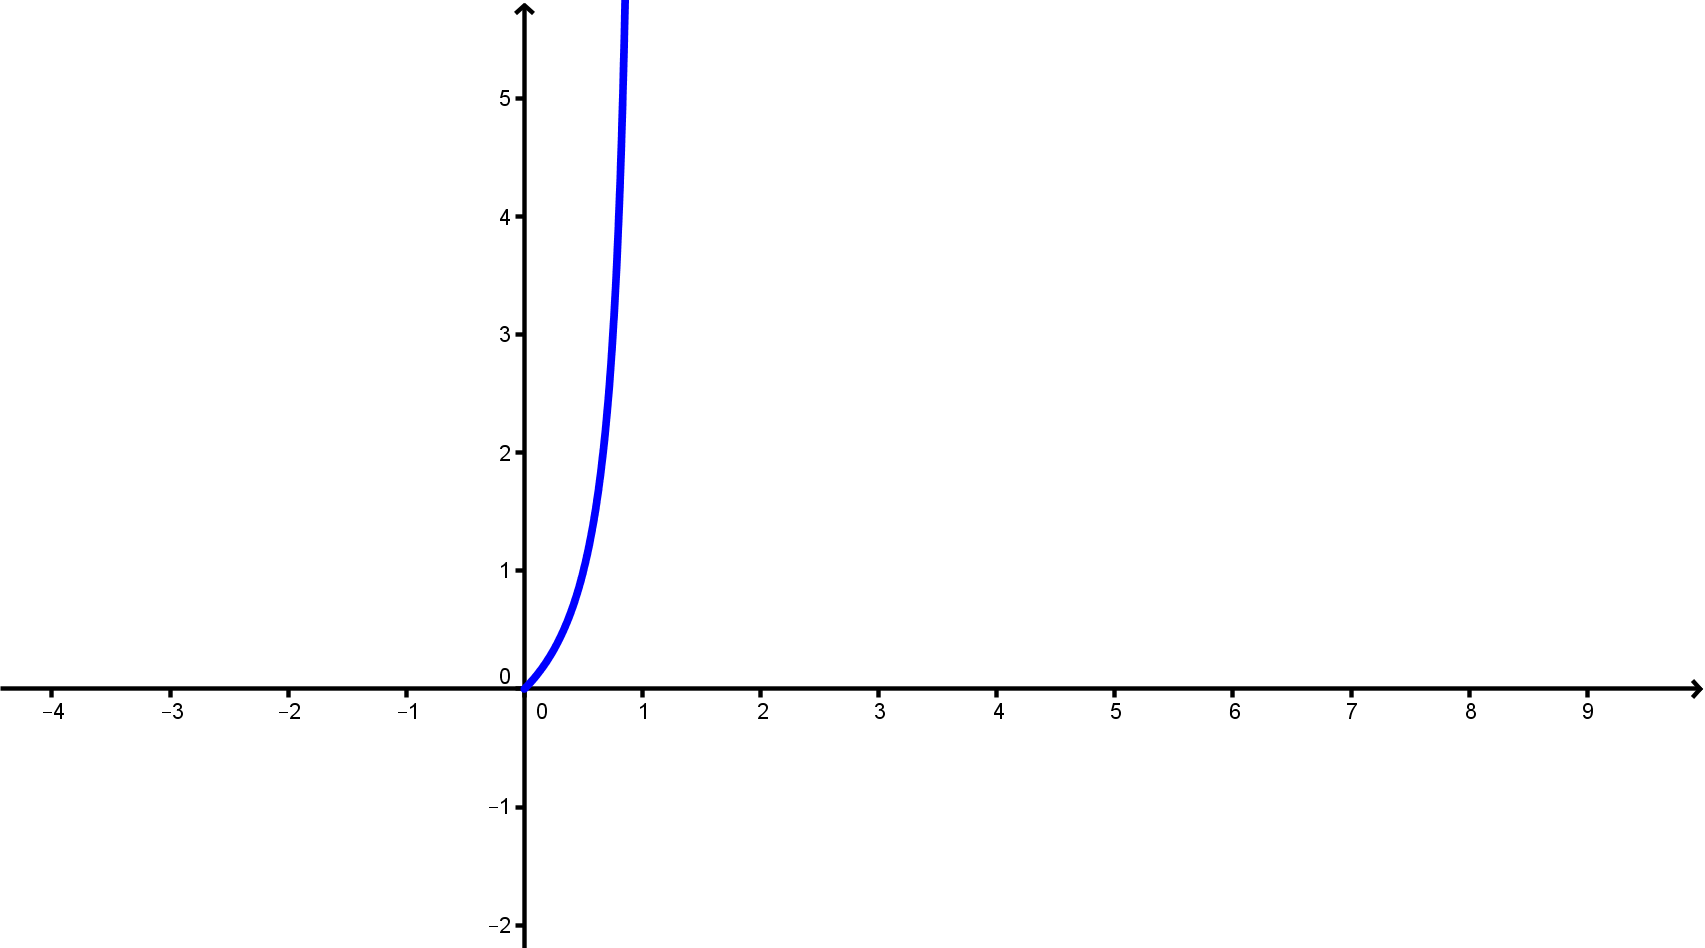
\includegraphics[width=10cm]{../fig/Cap03-OddsVsProbabilidad.png}
\end{enColor}
\begin{bn}
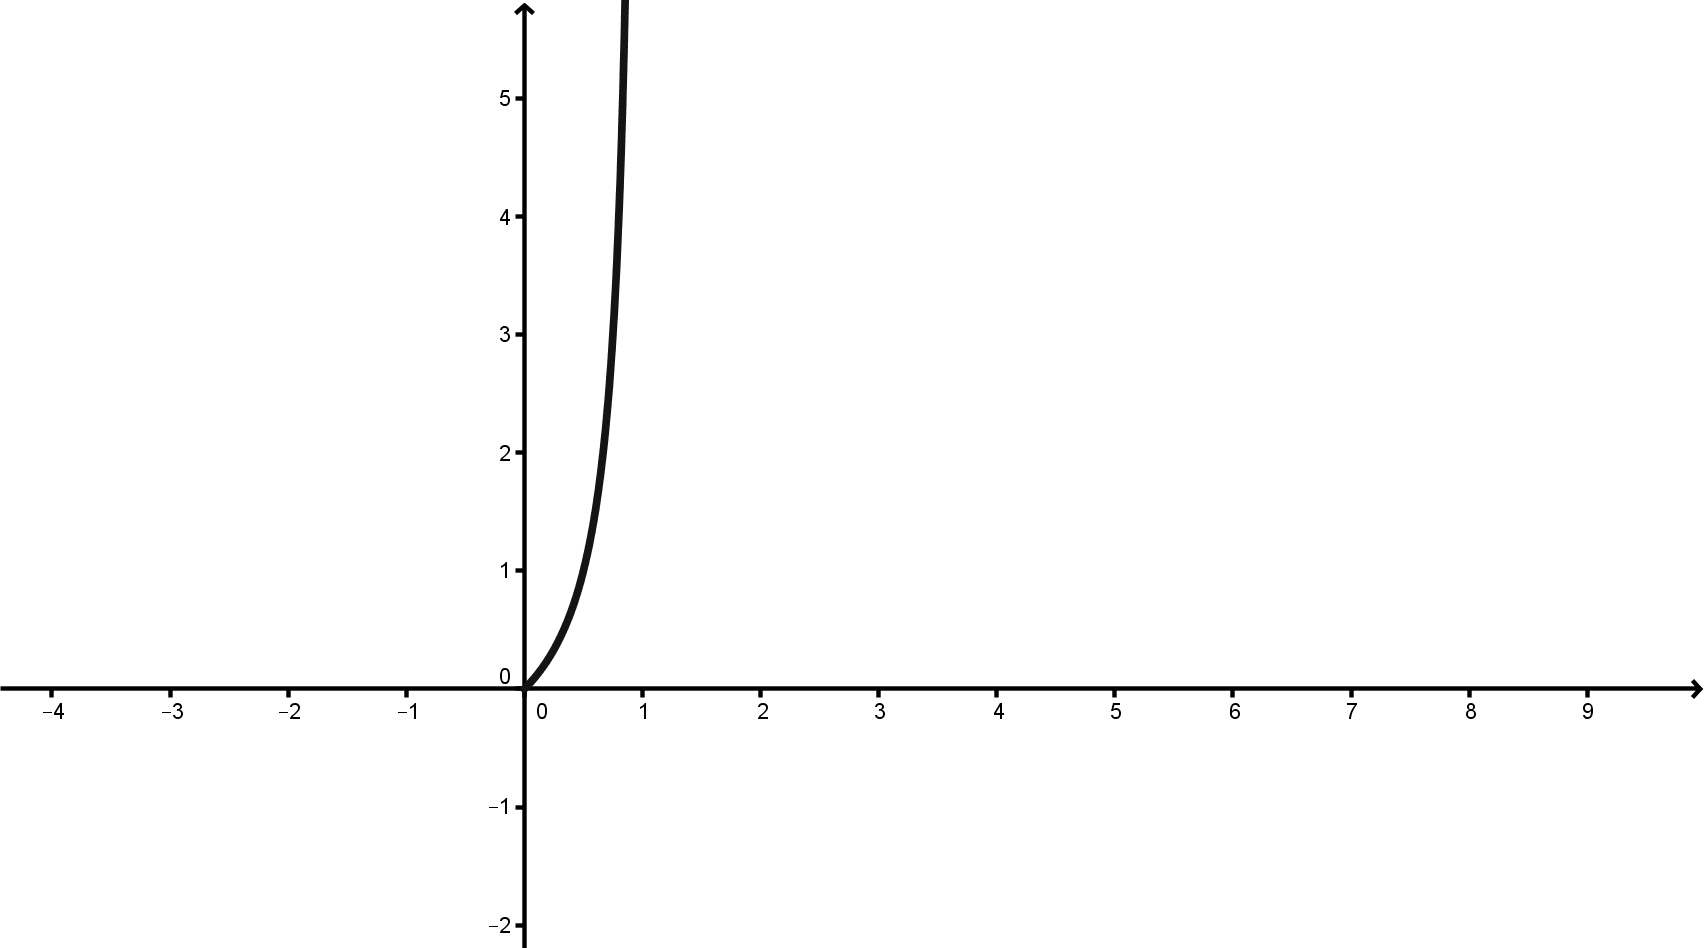
\includegraphics[width=10cm]{../fig/Cap03-OddsVsProbabilidad-bn.png}
\end{bn}
  \caption{Relación entre probabilidad (en el eje horizontal) y posibilidades (odds, en el eje vertical).}
  \label{cap12:Fig:OddsVsProbabilidad}
\end{center}
\end{figure}




\subsubsection*{Y entonces, ¿cómo funcionan las apuestas?}

Aunque no lo necesitamos estrictamente para nuestro trabajo, vamos a aprovechar para explicar el mecanismo de las {\sf apuestas basadas en posibilidades (odds)}\index{apuestas}.  La complicación adicional, en este caso, es que los apostadores a menudo utilizan las {\em posibilidades en contra} a la hora  de describir una apuesta.

Para fijar ideas, vamos a suponer que las apuestas están $7$ a $1$, {\em en contra de $A$}. En términos de posibilidades, eso significa:
\[
O_{A^c}=
\dfrac{\mbox{núm. de sucesos elementales favorables a $A^c$}}
{\mbox{núm. de sucesos elementales {\bf contrarios} a $A^c$}}=\dfrac{7}{1}.
\]
o, lo que es lo mismo,
\[
O_{A}=
\dfrac{\mbox{núm. de sucesos elementales {\bf contrarios} a $A$}}
{\mbox{núm. de sucesos elementales favorables a $A$}}
=\dfrac{1}{7}.
\]
Como puede deducirse, los apostadores creen que es siete veces más probable que ocurra $A^c$, frente a $A$. La apuesta por $A$, al ser más arriesgada, tiene un premio mucho mayor que la apuesta por $A^c$, que es la favorita de los apostadores. Una vez entendidas esas ideas, veamos cuales son las reglas que rigen las apuestas. Seguiremos con este ejemplo numérico para mayor claridad, y suponemos que las apuestas están $7$ a $1$ {\em en contra} de $A$:
\begin{itemize}
  \item Si yo apuesto por $A$, y ocurre $A$, eso quiere decir que, por cada euro que yo apuesto, me pagarán $7$ euros adicionales (además del que yo puse inicialmente). Naturalmente, si yo he apostado por $A$, y ocurre $A^c$, entonces pierdo el euro que aposté.
  \item  ¿Qué sucede si apuesto por $A^c$, cuando las apuestas están $7$ a $1$ {\em en contra} de  $A$? En este caso, en el que estoy apostando por el favorito, mis ganancias son el euro inicial, más $\frac{1}{7}$ de euro. Si apuesto por $A^c$, y gana $A$, de nuevo pierdo mi apuesta.
\end{itemize}
Para entender el razonamiento que hay detrás de estas reglas, tenemos que esperar hasta el Capítulo \ref{cap:VariablesAleatorias}, en el que, en la Sección \ref{cap04:subsec:VarianzaDesvTipicaVariableAleatoriaDiscreta} (pág. \pageref{cap04:subsec:VarianzaDesvTipicaVariableAleatoriaDiscreta}), introduciremos la idea de {\em juego justo}. Pero podemos ir adelantando algo del trabajo en un ejemplo:
\begin{ejemplo}
\label{cap03:ejem:OddsReglasApuestas}
Un corredor de apuestas sabe que siete apostadores quieren apostar, cada uno, un euro contra $A$, mientras que sólo un apostador está dispuesto a apostar un euro a favor de $A$. El apostador fija las apuestas $7$ a $1$ contra $A$, y reúne el dinero de los apostadores, que hace un total de $8$ euros.

Supongamos que ocurre $A^c$. Entonces el corredor de apuestas devuelve, a cada uno de los siete jugadores que apostaron contra $A$ el euro que apostaron, y usa el euro que se apostó a favor de $A$ para darles a esos jugadores un premio de $1/7$ de euro. El jugador que apostó a favor de $A$, naturalmente, ha perdido su euro.

Supongamos que ocurre $A$. Entonces el corredor de apuestas entrega, al único jugador que apostó por $A$, la totalidad de los ocho euros: su euro adicional, y los siete de los otros jugadores como premio. Los siete jugadores que apostaron contra $A$, naturalmente, han perdido su dinero.

En cualquier caso, el corredor de apuestas no pierde ni gana dinero, así que para él es básicamente indiferente quien gane o pierda. Naturalmente, los corredores de apuestas del mundo real quieren ganarse la vida con su negocio, así que las posibilidades (odds) que comunican a los jugadores tienen que incluir un cierto {\em sesgo} a su favor, para que ellos obtengan algún beneficio.
\qed
\end{ejemplo}
Con esto, ya estamos listos para dejar el garito de los apostadores, y volver a las pruebas diagnósticas.

%\subsubsection*{Posibilidades (odds) vs. probabilidades.}
%
%Si decimos que $O_A=7$, ¿cuál es nuestra estimación de la probabilidad de que $A$ gane? La idea es que $O_A=7$ significa que $B$ se considera $7$ veces más probable que $A$.  Y esto es lo que nos permite relacionar ambos conceptos. Si llamamos, como siempre, $P(A)$ y $P(B)$, a las probabilidades de $A$ y $B$ respectivamente, decir que $O_A=7$ significa que:
%\[P(B)=7\cdot P(A).\]
%Por otra parte, estamos suponiendo que $B=A^c$, de modo que
%\[1=P(A)+P(B),\]
%y por lo tanto:
%\[1=P(A)+7\cdot P(A)=8\cdot P(A).\]
%Es decir,
%\[P(A)=\dfrac{1}{8}.\]
%Repitiendo este razonamiento en general, se obtiene:
%\[P(A)=\dfrac{1}{1+O_A},\]
%y de aquí obtenemos la definición general.
%    \begin{center}
%    \fcolorbox{black}{Gris025}{
%    \begin{minipage}{12cm}
%    \begin{center}
%    {\bf Posibilidades (odds) de un suceso.}
%    \end{center}
%    Sea $A$ un suceso. Cuando decimos que el número $O_A$ representa las posibilidades a favor ({\em odds in favor}) del suceso $A$, eso equivale a decir que
%    \begin{equation}\label{cap03:ecu:OddsVsProbabilidades}
%    P(A)=\dfrac{1}{1+O_A}.
%    \end{equation}
%    Recíprocamente, dada la probabilidad $P(A)$, las posibilidades a favor de $A$ son:
%    \begin{equation}\label{cap03:ecu:ProbabilidadesVsOdds}
%    O_A=\dfrac{1}{P(A)}-1=\dfrac{1-P(A)}{P(A)}=\dfrac{P(A^c)}{P(A)}.
%    \end{equation}
%    \end{minipage}}
%    \end{center}
%
%Si decimos que
%
%
%La clave es entender la idea de {\em media o valor esperado}. En principio, una apuesta sólo se puede ganar o perder. Por lo tanto, se basa en una variable aleatoria de tipo Bernouilli (llamémosla $A$), con probabilidad $p$ de perder (de que yo pierda el dinero que he apostado) y $q=1-p$ de ganar. Supongamos que las proporciones para esta apuesta son de $k$ euros a 1. Es decir, si gano recibo $k$ euros por cada euro apostado (mientras que si pierdo, pierdo el euro que aposté, naturalmente). ¿Cuál es entonces el valor medio, o valor esperado de $A$? Pues sería
%\[\mu_A=q\cdot k+p\cdot(-1)\]
%El valor $-1$ en el segundo sumando corresponde a mis pérdidas (1 euro), si la suerte no me favorece.
%
%Dado este cálculo, ¿cuándo estamos ante una apuesta justa? Pues cuando mis ganancias esperadas son de cero euros (es decir, ni pierdo ni gano). Una apuesta justa debe cumplir:
%\[\mu_A=0\]
%Despejando de aquí, obtenemos una receta para calcular el valor $k$ que debería pagarnos el corredor de apuestas, una vez conocida la probabilidad $p$ de que yo gane la apuesta. En efecto, de
%\[0=q\cdot k+p\cdot(-1)\]
%se deduce
%\[
%k=\dfrac{p}{q}=\dfrac{p}{1-p}
%\]
%Esta relación entre proporciones (la cantidad $k$) y probabilidades no es del todo evidente. Por ejemplo, si la probabilidad de que yo pierda es del $80\%$ (es decir, $p=0.8$ y $q=0.2$) entonces, cuando gano, el corredor de apuestas debería pagarme
%\[
%k=\dfrac{0.8}{0.2}=4.
%\]
%euros por cada euro. Es una apuesta 4 a 1 si ha de ser justa. ¿Cuál debería ser el valor de $p$ para que la apuesta sea 10 a 1 (Calcúlalo; pero atención, {\sf no es el 90\%})?
%
%
%¿Qué tiene que ver toda esta terminología de apuestas con las pruebas diagnósticas? Supongo que el origen de todo es el hecho de que muchas personas (pacientes y/o personal sanitario) tienen problemas para entender el concepto de probabilidad. En cambio, la noción de proporciones (odds) en una apuesta es más conocida y familiar, para muchas de esas personas.
%
%La propia noción de prevalencia de una enfermedad se puede expresar, para ayudar a visualizarla, en términos de odds. Por ejemplo, si decimos que hay un enfermo de diabetes por cada 20 individuos sanos, {\bf no} estamos diciendo que la probabilidad sea
%\[\dfrac{1}{20}.\]
%Este número no es la probabilidad (prevalencia), sino la proporción. La prevalencia, es decir, la probabilidad, de hecho es (ahora debería ser evidente):
%\[\dfrac{1}{21}.\]
%Como vemos, la noción de odds o proporciones es simplemente otra forma de expresar la relación entre el número de enfermos y el total de la población.

\subsubsection*{Posibilidades (odds) pre y post diagnóstico.}

Una vez entendida la idea de posibilidades (odds), y para ver un ejemplo de su utilidad, vamos a aplicarla a las pruebas diagnósticas.  Como antes, llamamos $D$ al suceso {\em ``padecer la enfermedad''}, e indicaremos con los símbolos $+$ y $-$, los sucesos {\em ``prueba positiva''} y {\em ``prueba negativa''}, respectivamente.

Antes de realizar una prueba diagnóstica, ¿cuáles son las posibilidades (odds) de que el individuo esté enfermo? Es decir, las posibilidades a favor del suceso $D$. Usando la Ecuación \ref{cap03:ecu:OddsEnFuncionProbabilidades} (pág. \pageref{cap03:ecu:OddsEnFuncionProbabilidades}), se tiene:
\[\mbox{Posibilidades $D$ pre-prueba}=O_D=\dfrac{P(D)}{1-P(D)}\]
En inglés esta cantidad se describe como {\em pre-test odds}.

¿Y si ya hemos hecho la prueba, y el resultado ha sido positivo? ¿Cuánto valen ahora las posibilidades de $D$? Después de la prueba positiva, los valores relevantes son $P(D|+)$ y $P(D^c|+)$ (observa que estos dos valores también suman 1). Así que las probabilidades post-prueba (en inglés, {\em post-test odds})  pasan a ser:
\[\mbox{Posibilidades $D$ post-prueba}= \dfrac{P(D|+)}{P(D^c|+)}=\dfrac{P(D|+)}{1-P(D|+)}.\]
Lo que hace interesante estas expresiones es que las posibilidades pre y post prueba diagnóstica se pueden relacionar de forma muy sencilla con la razón de verosimilitud positiva $RVP$ de la Ecuación \ref{cap03:ecu:RazonVerosimilitudPositiva} (ver pág.\pageref{cap03:ecu:RazonVerosimilitudPositiva}; usamos $RVP$ porque la prueba ha sido positiva; si fuera negativa usaríamos $RVN$). Aquí es donde entra en acción el Teorema de Bayes. Por un lado, ese teorema nos dice que:
\[
P(D|+)=\dfrac{P(+|D)P(D)}{P(+|D)P(D)+P(+|D^c)P(D^c)}
\]
Y otra aplicación del teorema produce:
\[
P(D^c|+)=\dfrac{P(+|D^c)P(D^c)}{P(+|D^c)P(D^c)+P(+|D)P(D)}
\]
Ahora hay que darse cuenta de que, aunque el orden es distinto, los denominadores son iguales. Dividiendo las dos fracciones esos denominadores se cancelan y obtenemos, tras reorganizar un poco el resultado:
\[
\dfrac{P(D|+)}{P(D^c|+)}=\dfrac{P(+|D)}{P(+|D^c)}\cdot\dfrac{P(D)}{P(D^c)}.
\]
Teniendo en cuenta la terminología que hemos ido introduciendo, esto significa que (usamos odds en lugar de posibilidades para abreviar):
\begin{equation}\label{cap03:ecu:RelacionBayesianaOddsPrePostTestPositivo}
\left(\mbox{Odds $D$ post-prueba positiva}\right)=RVP\cdot \left(\mbox{Odds $D$ pre-prueba}\right).
\end{equation}
donde $RVP$ es, recordemos la Ecuación \ref{cap03:ecu:RazonVerosimilitudPositiva}, la razón de verosimilitud positiva de la prueba. Por un razonamiento análogo, se obtiene:
\begin{equation}\label{cap03:ecu:RelacionBayesianaOddsPrePostTestNegativo}
\left(\mbox{Odds $D$ post-prueba negativa}\right)=RVN\cdot \left(\mbox{Odds $D$ pre-prueba}\right).
\end{equation}
La Ecuación \ref{cap03:ecu:RelacionBayesianaOddsPrePostTestPositivo} permite, de una manera muy sencilla, actualizar nuestro cálculo de las posibilidades a favor de $D$, una vez obtenido un resultado positivo en la prueba. La relación entre ambas posibilidades es el factor $RVP$, la razón de verosimilitud positiva, que a su vez depende de la sensibilidad y la especificidad de la prueba.

\subsubsection{¿Qué es mejor, usar probabilidades o posibilidades (odds)?}
\label{cap03:subsubsec:QueEsMejorPosibilidadesProabilidades}

Ahora que ya sabemos qué son, y cómo se comportan las posibilidades, es posible que el lector se esté planteando la pregunta que encabeza este apartado. Y la mejor respuesta que podemos darle es que no hay una respuesta. Los dos objetos, posibilidades y probabilidades, son descripciones alternativas de una misma situación. Y tienen propiedades matemáticas distintas. Una probabilidad está obligada a permanecer en el intervalo $[0,1]$, y es muy fácil de convertir en un porcentaje. Por su parte, las posibilidades pueden tomar cualquier valor positivo (o infinito, si la probabilidad es $1$). Todavía no hemos avanzado suficiente en el curso para saber por qué a veces es preferible que suceda una de esas dos cosas. Pero la buena noticia es, sin duda, que no hay ninguna necesidad de elegir. Las probabilidades y las posibilidades son herramientas de las que disponemos. Es como si tuviéramos que elegir si es mejor un destornillador o una llave inglesa. Lo mejor, sin duda, es llevar las dos en la caja de herramientas, y usar la herramienta adecuada para cada problema.

\subsubsection{Verosimilitud}
\label{cap03:subsubsec:verosimilitud}

La idea de {\sf verosimilitud}\index{verosimilitud} (en inglés, {\em likelihood}\index{likelihood}) es una idea muy importante en Estadística. Ya la hemos usado en el nombre de $RVP$ y en las ecuaciones como \ref{cap03:ecu:RelacionBayesianaOddsPrePostTestPositivo} y \ref{cap03:ecu:RelacionBayesianaOddsPrePostTestNegativo}.  A lo largo del curso nos la vamos a encontrar varias veces, e iremos añadiendo detalles a nuestra comprensión del concepto. Por el momento, aprovechando nuestro contacto con el Teorema de Bayes, nos vamos a conformar con una idea muy general.

El método científico se basa, muy esquemáticamente, en observar la naturaleza, formular teorías y modelos sobre ella, y contrastar esas teorías con los datos empíricos. Naturalmente, puesto que las teorías son explicaciones {\em parciales} de la realidad, sus predicciones no son nunca absolutamente exactas. Siempre se incluye un cierto margen de error, un {\em ruido} o componente aleatoria más o menos pequeño. Obviamente, para que la teoría sirva de algo, ese error o ruido tiene que ser pequeño, comparado con las cantidades que intervienen. En ese sentido, nunca esperamos de los científicos una certidumbre absoluta (hay otras instancias que se encargan de ese negocio...). No, lo que se espera de una teoría científica es un {\em control adecuado del error}, entendido como un procedimiento para medir la magnitud de ese error. Usando el lenguaje de la probabilidad condicionada, podemos expresar así ese control:
\[P\left(\mbox{datos}\,|\,\mbox{teoría cierta}\right).\]
Es decir, la teoría tiene que ser capaz de responder a preguntas como: {\em ``si la teoría es cierta, ¿cuál es la probabilidad de observar ciertos datos concretos?''} Un ejemplo sencillo puede ayudar a entender esto: supongamos que mi teoría dice que el dado no está cargado (todos los valores son equiprobables). Entonces, puedo usar esa teoría para predecir, por ejemplo (y usando la Regla de Laplace)
\[P\left(\mbox{resultado = }5\,|\,\mbox{teoría = ``dado no cargado''}\right)=\dfrac{1}{6}.\]
El otro componente esencial del método científico es la comparación de la teoría con los datos. Si, después de lanzar $1000$ veces el dado, el $5$ sólo hubiera aparecido $10$ veces, mi teoría de que el dado no está cargado se vería en un serio aprieto. En esta parte del trabajo, la pregunta que nos interesa tiene más que ver con la probabilidad condicionada recíproca de la anterior:
\[P\left(\mbox{teoría cierta}\,|\,\mbox{datos}\right).\]
Piénsalo así: dados los datos ($1000$ lanzamientos en los que el $5$ sólo aparece $10$ veces), ¿cuál es la probabilidad de que la teoría (``el dado no está cargado'') sea cierta? Ese valor no es $0$, desde luego. Pero es un valor tan ridículamente pequeño, que nadie en sus cabales seguiría creyendo en la teoría después de observar esos datos. Para describir lo que esperamos de la Ciencia, nos viene a la mente esa frase frecuente en el sistema judicial anglosajón: ``más allá de cualquier duda razonable'' (en inglés {\em ``beyond a reasonable doubt''}).

La relación entre las dos probabilidades condicionadas anteriores, viene determinada por el Teorema de Bayes:
\[
P(\mbox{teoría cierta}|\mbox{datos})=
\dfrac{
P(\mbox{datos}|\mbox{teoría cierta})\cdot P(\mbox{teoría cierta})}{P(\mbox{datos})}.
\]
que se puede expresar así:
\begin{equation}
\label{cap03:ecu:FuncionVerosimilitudBayes}
\underbrace{
P(\mbox{teoría cierta}|\mbox{datos})}_{\mbox{\tiny después de los datos}}=
\dfrac{\mathcal{L}(\mbox{datos, teoría cierta})}{P(\mbox{datos})}
\cdot
\underbrace{
P(\mbox{teoría cierta})}_{\mbox{\tiny antes de los datos}}
,\end{equation}
donde $\mathcal{L}(\mbox{datos, teoría cierta})=P(\mbox{datos}|\mbox{teoría cierta})$ es la {\sf función verosimilitud}\index{función verosimilitud}\index{verosimilitud, función}. Como hemos indicado, el término $P(\mbox{teoría cierta})$ indica nuestro grado de creencia en la teoría antes de ver los datos. Y el término de la izquierda, $P(\mbox{teoría cierta}|\mbox{datos})$ nos dice cómo ha cambiado esa creencia una vez examinados los datos. El cociente que los relaciona es un {\em artefacto estadístico}, es la forma en la que la Estadística nos ayuda a actualizar nuestras creencias sobre esa teoría. En particular, esa actualización pasa por comparar nuestra teoría con las posibles teorías alternativas. Por eso la teoría aparece como una variable de la función de verosimilitud, porque vamos a considerar distintas teorías. En próximos capítulos iremos conociendo esta función en más detalle.

La Ecuación \ref{cap03:ecu:FuncionVerosimilitudBayes} resume (de manera muy simplificada) el proceso por el que el método científico actualiza su confianza en una teoría. Podemos verlo de esta manera: tenemos una teoría que deseamos someter a escrutinio, y acabamos de obtener una colección de datos. A la izquierda, de la Ecuación \ref{cap03:ecu:FuncionVerosimilitudBayes} está la pregunta a la que queremos responder: ``¿qué probabilidad hay de que esa teoría sea cierta, a la luz de estos datos?'' La respuesta, tal como nos la proporciona el lado derecho de la Ecuación \ref{cap03:ecu:FuncionVerosimilitudBayes}, tiene tres ingredientes:
\begin{itemize}
  \item $P(\mbox{teoría cierta})$, es una medida de nuestra confianza en esa teoría {\em previa} a la aparición de esos datos. A menudo se dice que es la probabilidad {``a priori''}\index{a priori} (en inglés {\em prior probability}) o, simplemente, {\em prior}.
  \item $\mathcal{L}(\mbox{datos, teoría cierta})$ es el valor de la función verosimilitud, cuando la teoría es cierta. Podríamos decir que aquí es donde entra en juego la Estadística, que nos tiene que decir cual es esa función.
  \item La probabilidad $P(\mbox{datos})$ representa la probabilidad (absoluta, no condicionada) de los datos, y es la parte menos accesible para nosotros de esta expresión.
\end{itemize}
Precisamente por esta última observación, la función de verosimilitud se lleva especialmente bien con la idea de posibilidades (odds).  Si escribimos la ecuación análoga a \ref{cap03:ecu:FuncionVerosimilitudBayes} para el cálculo de la probabilidad de que la teoría sea falsa (con los mismos datos), tenemos:
\[
P(\mbox{teoría falsa}|\mbox{datos})=
\dfrac{\mathcal{L}(\mbox{datos, teoría cierta})}{P(\mbox{datos})}
\cdot P(\mbox{teoría falsa})
\]
Y si dividimos la Ecuación \ref{cap03:ecu:FuncionVerosimilitudBayes} por esta ecuación tenemos:
\begin{equation}
\label{cap03:ecu:CocienteVerosimilitudes}
%O(\mbox{teoría falsa}|\mbox{datos})=
\dfrac{P(\mbox{teoría cierta}|\mbox{datos})}{P(\mbox{teoría falsa}|\mbox{datos})}=
\dfrac{\mathcal{L}(\mbox{datos, teoría cierta})}{\mathcal{L}(\mbox{datos, teoría falsa})}
\cdot
\dfrac{P(\mbox{teoría cierta})}{P(\mbox{teoría falsa})}.
\end{equation}
El último término de la derecha de esta ecuación son las posibilidades a favor de que la teoría sea cierta {\em a priori}. Vienen a representar nuestra confianza en esa teoría antes de conocer los datos. Para ver esto, sólo hay que tener en cuenta que {\em teoría cierta} y {\em teoría falsa} son complementarios, y recordar la definición \ref{cap03:ecu:ProbabilidadesEnFuncionOdds} (pág. \pageref{cap03:ecu:ProbabilidadesEnFuncionOdds}). De la misma forma, el término de la izquierda son las posibilidades (odds) a favor de que la teoría sea cierta, {\em a posteriori}; es decir, una vez que tenemos en cuenta los datos. Y como se ve, el mecanismo para actualizar nuestra visión de la validez de esa teoría es el {\sf cociente o razón de verosimilitudes}\index{cociente de verosimilitudes}\index{verosimilitudes, cociente o razón} (en inglés {\em likelihood ratio}\index{likelihood ratio}). Fíjate, en particular, en que este enfoque elimina el término $P(\mbox{datos})$ que nos causaba problemas. Por tanto, podemos escribir así la Ecuación \ref{cap03:ecu:CocienteVerosimilitudes}:

\begin{equation}
\label{cap03:ecu:OddsCocienteVerosimilitudes}
%O(\mbox{teoría falsa}|\mbox{datos})=
O_{\mbox{teoría cierta}|\mbox{datos}}=
\dfrac{\mathcal{L}(\mbox{datos, teoría cierta})}{\mathcal{L}(\mbox{datos, teoría falsa})}
\cdot
O_{\mbox{teoría cierta}}
\end{equation}

Conviene, además, comparar esta Ecuación \ref{cap03:ecu:CocienteVerosimilitudes} con las Ecuaciones \ref{cap03:ecu:RelacionBayesianaOddsPrePostTestPositivo} y \ref{cap03:ecu:RelacionBayesianaOddsPrePostTestNegativo} (pág. \pageref{cap03:ecu:RelacionBayesianaOddsPrePostTestPositivo}), para ver que su estructura es la misma. Para hacer la analogía más completa, puedes pensar que en el caso de las pruebas diagnósticas la teoría es el suceso que hemos llamado $D =${\em ``el paciente está enfermo''}, mientras que los datos son el suceso que hemos llamado $+ = ${\em ``el diagnóstico es positivo''.}

Seguramente esta discusión tan genérica puede resultar un poco desconcertante, al menos la primera vez. Hasta cierto punto, es inevitable que así sea; por la novedad, y porque nuestra experiencia con la idea de verosimilitud, a estas alturas del curso, es mínima. En próximos capítulos volveremos sobre esa idea varias veces, y las cosas irán quedando cada vez más claras.

%\section{Ejercicios para practicar estas ideas}
%
%
%\begin{enumerate}
%
%    \item  En un estudio en el que se incluyen 1000 pacientes enfermos y 100 no enfermos, una prueba diagnostica clasifica como positivos al 70\% de los enfermos, y como negativos al 95\% de los no enfermos. Calcular la sensibilidad y la especificidad de la prueba.
%
%    \item  La sensibilidad de una prueba diagnóstica es $0.95$ y su especificidad es $0.85$. Si la prevalencia de la enfermedad es $0.002$, ¿cuál es el valor predictivo positivo del test?
%
%    \item En la información que describe un test de embarazo se puede leer ``Cuando los usuarios del test son mujeres que recogen y ensayan sus propias muestras, la sensibilidad del test es del 75\%. La especificidad también es baja, de entre un 52\% y un 75\%.'' Aceptando el valor más bajo para la especificidad, ¿cuánto vale la razón de verosimilitud diagnóstica negativa de este test? Vamos a suponer que una mujer ha obtenido un resultado negativo en el test. Sabiendo que un 30\% de las mujeres que realizan pruebas de embarazo están de hecho embarazadas, ¿cuál es la probabilidad de que esta mujer lo esté?
%
%    \item Un estudio que compara la eficacia de varias pruebas diagnósticas del VIH describe un experimento en el que se obtuvo que los test de anticuerpos del VIH tienen una sensibilidad del 99.7\% y una especificidad del 98.5\%. Supongamos queun individuo, dentro de una población con una prevalencia del 0.1\%  de VIH, obtiene un resultado positivo en uno de estos test de anticuerpos. ¿Cuál es la probabilidad de que realmente tenga el VIH? ¿Cuál es el valor predictivo positivo de este test?
%
%    \item La siguiente tabla muestra los resultados de un test de diagnóstico que se utilizó con dos muestras independientes de 650 sujetos enfermos y 1200 sujetos sanos.
%
%        \begin{center}
%            \begin{tabular}{llccc}
%            &&\multicolumn{3}{c}{\underline{\bf Estado real}}\\
%
%                                  &          & Enfermos & Sanos& \\
%            \hline
%  \underline{\bf Resultado del test}          & Positivo & 490 & 70   &   \\
%                                              & Negativo & 160 & 1130 &   \\
%            \hline
%                                              &          &     &     &    \\
%            \hline
%            \end{tabular}
%        \end{center}
%        Calcular la sensibilidad y la especificidad del test. Si la prevalencia de la enfermedad es $0.002$, ¿cuál es el valor predictivo positivo del test?
%
%
%    \item Los resultados de la siguiente tabla se obtuvieron en un estudio diseñado para averiguar la capacidad de un cirujano anatomopatólogo para clasificar correctamente biopsias quirúrgicas en malignas o benignas. Aproximar $\alpha$ y $\beta$ a partir de estos datos.
%
%        \begin{center}
%            \begin{tabular}{llccc}
%            &&\multicolumn{3}{c}{\underline{\bf Estado real}}\\
%
%                                  &          & Benigno (-)& Maligno (+)& Total\\
%            \hline
%  \underline{\bf Informe del anatomopatólogo} & Positivo & 7 & 79   &   \\
%                                              & Negativo & 395  & 19 &   \\
%            \hline
%                                              &          &     &     & 500  \\
%            \hline
%            \end{tabular}
%        \end{center}
%
%    \item Se está ensayando un nuevo método para detectar enfermedades renales en pacientes con hipertensión. Se aplica el nuevo procedimiento a 137 pacientes hipertensos. Y a continuación, a esos mismos pacientes se les aplica un método anterior, bien contrastado, para comprobar la presencia o ausencia de enfermedad renal. Los datos obtenidos se recogen en la tabla. Utilizando estos datos, calcular aproximadamente la probabilidad de falso positivo y la de falso negativo del nuevo método. Aproximar asimismo el valor predictivo positivo y el valor predictivo negativo del nuevo método.
%
%        \begin{center}
%            \begin{tabular}{llccc}
%            &&\multicolumn{3}{c}{\underline{\bf Estado real (método clásico)}}\\
%
%                                  &          & Sano (-)& Enfermo (+)& Total\\
%            \hline
%            \underline{\bf Nuevo método}     & Enfermo (+) & 23  & 44 &   \\
%                                             & Sano (-) & 60  & 10 &   \\
%            \hline
%                                              &          &     &     & 137  \\
%            \hline
%            \end{tabular}
%        \end{center}
%
%\item En la siguiente tabla se muestran los resultados de un estudio para evaluar la utilidad de una tira reactiva para el diagnóstico de infección urinaria.
%        \begin{center}
%            \begin{tabular}{llccc}
%            &&\multicolumn{3}{c}{\underline{\bf Estado real}}\\
%
%                                  &          & Con infección& Sin infección&\\
%            \hline
%            \underline{\bf Tira reactiva}     & Positivo & 60  & 80 &   \\
%                                             & Negativo & 10  & 200 &   \\
%            \hline
%                                              &          &     &     & 350  \\
%            \hline
%            \end{tabular}
%        \end{center}
%        Calcular e interpretar sensibilidad y especificidad, y los valores predictivos positivo y negativo. Si conocemos que la prevalencia de la infección en la población de interés es del 2\%, ¿cómo se verían afectados los valores predictivos? ¿Es esta tira reactiva una buena prueba diagnóstica?
%
%\end{enumerate}
